\documentclass[final,3p,times]{elsarticle}
\usepackage[tensorialbold]{userCommands}
\usepackage[american]{babel}
\usepackage[font=normal]{caption}
\usepackage[font=normal]{subcaption}
\usepackage{tikz} % geometrical figures
\usetikzlibrary{calc,trees,positioning,arrows,chains,shapes.geometric,decorations.pathreplacing,decorations.pathmorphing,shapes,
    matrix,shapes.symbols,shapes.multipart,patterns,shapes,snakes,pgfplots.groupplots,spy,backgrounds}
\usetikzlibrary{external}
\tikzexternalize[prefix=external/]
\usetikzlibrary{spy,backgrounds}
\usetikzlibrary{decorations.markings}
\usetikzlibrary{arrows.meta}

\usepackage{pgfplots} % pdf picture declaration

\usepackage{array}
\newcolumntype{M}[1]{>{\centering\arraybackslash}m{#1}}
\newcolumntype{N}{@{}m{0pt}@{}}


%% The amssymb package provides various useful mathematical symbols
\usepackage{amssymb}
\usepackage{lineno}
%\linenumbers

\usepackage{float}
%\usepackage[section]{placeins} % pictures restricted to \section

% \makeatletter % restriction of figures to subsections as well (not managed by the package) 
% \renewcommand\subsection{\FloatBarrier\@startsection{subsection}{2}{\z@}%du book.cls
% {-3.25ex\@plus -1ex \@minus -.2ex}%
% {1.5ex \@plus .2ex}%
% {\normalfont\large\bfseries}}
% \makeatother 


\usepackage{mathtools}
\mathtoolsset{showonlyrefs}

\journal{Computer Methods in Applied Mechanics and Engineering}

\pgfplotsset{%compat=1.3,
  %compat=1.8,
  compat=newest,
  grid=both,
  tick label style={font=\normalsize},
  label style={font=\normalsize},
  legend style={font=\normalsize},
  legend cell align={left},
  yticklabel style={/pgf/number format/fixed},
  %scaled y ticks=false,
  % define user colormap
  colormap={tol}{[1cm] rgb255(0cm)=(120,28,129) rgb255(1cm)=(63,96,174) rgb255(2cm)=(83,158,182) rgb255(3cm)=(109,179,136) rgb255(4cm)=(202,184,67) rgb255(5cm)=(231,133,50) rgb255(6cm)=(217,33,32)}
}

\definecolor{Purple}{RGB}{120,28,129}
\definecolor{Orange}{RGB}{231,133,50}
\definecolor{Blue}{RGB}{63,96,174}
\definecolor{Red}{RGB}{217,33,32}
\definecolor{Duck}{RGB}{83,158,182}
\definecolor{Green}{RGB}{109,179,136}
\definecolor{Yellow}{RGB}{202,184,67}

\newcommand{\review}[1]{\color{Red}#1\color{black}}

\newtheorem{remark}{Remark}


\begin{document}

\begin{frontmatter}


  %% Title, authors and addresses

  %% use the tnoteref command within \title for footnotes;
  %% use the tnotetext command for theassociated footnote;
  %% use the fnref command within \author or \address for footnotes;
  %% use the fntext command for theassociated footnote;
  %% use the corref command within \author for corresponding author footnotes;
  %% use the cortext command for theassociated footnote;
  %% use the ead command for the email address,
  %% and the form \ead[url] for the home page:
  %% \title{Title\tnoteref{label1}}
  %% \tnotetext[label1]{}
  %% \author{Name\corref{cor1}\fnref{label2}}
  %% \ead{email address}
  %% \ead[url]{home page}
  %% \fntext[label2]{}
  %% \cortext[cor1]{}
  %% \address{Address\fnref{label3}}
  %% \fntext[label3]{}
  
  %\title{Solving hyperbolic problems in hyperelastic-plastic solids with the Discontinuous Galerkin Material Point Method}
  \title{The Discontinuous Galerkin Material Point Method for variational hyperelastic-plastic solids.}
  
  %% use optional labels to link authors explicitly to addresses:
  %% \author[label1,label2]{}
  %% \address[label1]{}
  %% \address[label2]{}
  
  \author{Adrien Renaud$^1$, Thomas Heuz{\'e}, Laurent Stainier}
  
  \address{$^1$ Research Institute in Civil and Mechanical Engineering (GeM, UMR 6183 CNRS)\\
    Ecole Centrale de Nantes \\
    1 rue de la No\"e, Nantes\\
    e-mail: \{adrien.renaud,thomas.heuze,laurent.stainier\}@ec-nantes.fr}
  
  \begin{abstract}
    % In this paper, the formulation of the Discontinuous Galerkin Material Point Method is presented in the context of hyperbolic problems in the finite deformation framework.
    % The method, which is based on the discretization of a solid domain by means of particles in a background mesh, takes advantage of the finite volume and finite element technologies in order to track waves in solids undergoing large deformations.
    % On the one hand, the computational grid is used as a support for the discontinuous Galerkin approximation, which gives rise to fluxes computed through the solution of Riemann problems between the cells.
    % On the other hand, the set of particles is used to represent the geometry and for storing the fields of the problem, thus giving the grid its arbitrary nature for it can then be discarded and reconstructed for convenience.
    % Moreover, constitutive equations are dealt with at the particle level so that classical integrators can be employed.
    % It is proposed here to couple the DGMPM with constitutive integrators based on a variational reformulation of the continuum equations for hyperelastic-plastic solids.
    % The total Lagrangian formulation of the approach is then illustrated on numerical simulations for which comparisons with the finite element and material point methods, as well as exact solution in the linearized geometrical limit, are shown.
    The Discontinuous Galerkin Material Point Method (DGMPM), presented in \cite{DGMPM}, is based on the discretization of a solid domain by means of particles in a background mesh.
    This method aims at taking advantage of the finite volume and finite element technologies in order to track waves in solids undergoing large deformations.
    On the one hand, the computational grid is used as a support for the discontinuous Galerkin approximation, which gives rise to fluxes computed through the solution of Riemann problems between the cells.
    On the other hand, the set of particles is used to represent the geometry and for storing the fields of the problem, thus giving the grid its arbitrary nature for it can be discarded and reconstructed for convenience.
    Moreover, constitutive equations are dealt with at the particle level so that classical integrators can be employed.
    It is proposed in this paper to couple the DGMPM with variational integrators of hyperelastic-plastic constitutive models.
    \review{This class of integrators enables (i) strongly thermomechanically coupled problems (ii) mesh adaption (iii) }
    The total Lagrangian formulation of the approach is then illustrated on numerical examples for which comparisons are shown with the finite element and the material point methods, as well as exact solution in the linearized geometrical limit.
  \end{abstract}
  
  \begin{keyword}
    Discontinuous Galerkin Material Point Method; hyperelastic-plastic solids; variational constitutive update; impacts
  \end{keyword}
  
\end{frontmatter}



\section{Introduction}
\label{sec:introduction}
The numerical simulation of physical problems modeled by means of hyperbolic partial differential equations involves the solution of possibly discontinuous waves.
%
The precise tracking of those waves is of major importance in solid mechanics, especially for history-dependent constitutive equations, as it allows to properly assess the residual states.
\review{More specifically, high-speed forming techniques such that electromagnetic forming \cite{Formage} also requires the tracking of solid interfaces.}   
% \note{(a) Examples of applications that involve large deformations}
% \note{Discontinuities + Large deformations!!}
%
Nevertheless, the accurate simulation of such problems can be prevented by several reasons.
%% Mesh-based Lagrangian
First, Lagrangian formulations of mesh-based approaches such as the widely used Finite Element (FEM) \cite{Belytschko} and Finite Volume (FVM) \cite{Leveque} methods become less accurate for very large deformations due to sever distortions of the mesh.
%% Mesh-based Eulerian and ALE
Although those instabilities can be avoided by resorting to Eulerian or Arbitrary Lagrangian-Eulerian formulations, other difficulties arise owing to additional diffusive projections of fields.
%% Time integration
Second, it is well-known that explicit finite element schemes can exhibit numerical noise near sharp solutions that can be hard to remove with artificial viscosity without loss of accuracy.
Such oscillations can nevertheless be removed from FVM solutions due to numerical fluxes involved in the formulation, allowing the building of Total Variation Diminishing (TVD) schemes \cite{Harten}.
%% DG
The Discontinuous Galerkin approximation in space \cite{NeutronDG}, combined with FEM (DGFEM), enables to take advantage of similar interface fluxes so as to construct Total Variation Diminishing in the Means (TVDM) finite element procedures \cite{Cockburn}.
%% Time integration in DGFEM -> STDG
While the introduction of the DG approximation within FEM schemes enables to avoid non-physical oscillations, providing the use of suitable limiters \cite{vanLeer_Limiters}, these approaches are constrained by a restrictive CFL condition \cite{DGFEM_CFL} and hence, suffer from numerical diffusion.
Space-time DGFEM formulations \cite{ST_DGFEM1} enable to circumvent this drawback but are nonetheless subject to mesh entanglement.
%\review{Moreover, the satisfaction of the compatibility condition between reference and updated configurations, through the Piola identity, is not a straightforward undertaking in Lagrangian formulations \cite{Vilar_PiolaIdentity,LagrangianDG_thesis}, which is also the case for finite volumes \cite{Haider_FVM}.
%In other words, updating the geometry based on discontinuous velocities and deformation gradients across element faces may lead to discontinuities in the displacement vector.}


%% MPM
One possibility to avoid mesh tangling instabilities while providing a material description of the motion is to use mesh-free approaches such as those of the Particle-In-Cell (PIC) family \cite{PIC} and, in particular, the Material Point Method \cite{Sulsky94}.
The MPM is based on a dual discretization of a domain made of a collection of material points lying in an arbitrary grid.
A discrete system is solved on the grid, whereas the loading history is stored at particles during the motion so that field projections, which introduce some freedom into the scheme, are required.
%
Indeed, the updated velocity at the grid level can be directly interpolated to the particles according to the original PIC procedure.
Alternatively, the particle velocities can be updated by interpolating the nodal acceleration resulting from the solution of the discrete system, as introduced in PIC by the FLuid Implicit Particle method (FLIP) \cite{FLIP}.
The latter allows to reduce numerical diffusion at the cost of spurious oscillations \cite{PIC_Nishiguchi}.
Recently, a tunable mapping procedure, based on a parameter $m$ that completely eliminates the noise in MPM solutions, has been proposed in the Extended PIC of order $m$ (XPIC(m)) \cite{XPIC}.
A classical interpolation is selected for $m=1$ whereas the mapping tends to FLIP one as $m\rightarrow \infty$.
Nevertheless, the numerical diffusion still prevents from capturing (discontinuous) waves.

%% DGMPM 
\review{
  %A different point of view, which is followed in the Discontinuous Galerkin Material Point Method (DGMPM) \cite{DGMPM,Thesis}, is that the numerical diffusion exhibited by the PIC can be limited by reducing the domain of influence of nodes rather than modifying the projections themselves.
  Note also that the numerical diffusion exhibited by the PIC can be limited by reducing the domain of influence of nodes rather than modifying the projections themselves.
  This approach is followed in the Discontinuous Galerkin Material Point Method (DGMPM) \cite{DGMPM,Thesis}.
  The introduction of the DG approximation within the MPM, combined with the use of the PIC projection, thus aims at providing non-oscillating discontinuous solutions with low numerical diffusion due to the support of the shape functions that reduces to one cell.
  Therefore, the DGMPM enables to take advantage of space-DGFEM and MPM in order to accurately follow waves in finite-deforming media.
}
%
In that method, the weak form of a system of conservation laws is written on an arbitrary grid and numerical fluxes arising from the DG approximation are computed at cell faces by means of an approximate Riemann solver.
Those intercell fluxes allow to take into account the characteristic structure of hyperbolic problems, and in particular the transverse propagation of waves through the use of the Corner Transport Upwind method (CTU) \cite{Colella_CTU} developed for finite volumes.
The CTU is however reformulated in order to fit the DGMPM approximation, in which fields are edge-wise constant in Riemann problems rather than cell-wise constant as it is the case for FVM.
%% Arbitrary grid
Furthermore, as in MPM, all the fields are stored at material points moving in the arbitrary grid, the mapping between nodes and particles being made with PIC projection so that non-oscillating solutions are provided.
\review{Hence, the geometry is updated at the particles level based on a single-valued velocity field. %, in such a way that the difficulties related to the Piola identity are expected to vanish, though it has not been shown so far.
  %% Total Lagrangian
  As a first development step, the DGMPM has been constructed upon a total Lagrangian formulation.
  %
  The numerical results provided by the method for a plane wave problem in a finite-deforming hyperelastic material showed excellent agreement with the exact solution consisting of either a shock or a rarefaction wave \cite{DGMPM}.
  It is worth noticing that similar results can be obtained with the FVM written in the reference configuration, the key point being however that the update of the geometry is straightforward in the DGMPM.
  %
  Furthermore, an interesting feature of the method consists in allowing the employment of mesh adaption strategies so that waves can be accurately captured in the current configuration.
  On the other hand, only linear shape functions leading to a first-order accuracy \cite{Thesis} have been considered, the extension of the method to higher-order approximations being the object of ongoing works.
  The low-order approximation is however not seen as a shortcoming for now since the development of the method has been focused so far on capturing discontinuous solutions for which the accuracy of any numerical scheme falls to one \cite{Leveque}.
}
%Although the equations of solid mechanics are solved in the reference configuration according to a total Lagrangian formulation, an interesting feature of the method consists in allowing the employment of mesh adaption strategies so that waves can be accurately captured in the current configuration.
%% CFL depending on the space discretization
Nonetheless, the stability of the DGMPM highly depends on the distribution of particles inside the computational grid.
Indeed, the stability analysis of the one-dimensional DGMPM scheme coupled to the forward Euler time integration \cite{DGMPM} yields a stability condition that depends on the space discretization and the CFL number.
%
Conversely, one can ensure the stability for a given distribution of material points by finding the CFL number satisfying the aforementioned relation.
%
Such a condition, which does not exist for the MPM and other DGMPM discretizations, is crucial since it allows to: (i) ensure the stability of the scheme while minimizing the numerical diffusion; (ii) adapt the Courant number when the grid is reconstructed; (iii) adapt the grid so that a given CFL condition is satisfied.
It is the purpose of this paper to provide the stability conditions for the one-dimensional DGMPM scheme combined with the two-stage second-order Runge-Kutta (RK2) time discretization and for the two-dimensional DGMPM coupled to the forward Euler algorithm.
\review{
  Although the solution of linear equations is considered here, the results presented must be put into the context of the problems aimed by the method, involving large deformation, and for which the DGMPM enables plenty of perspectives. 
  }

%% Organization of the paper
In the following, the DGMPM discrete system for the multi-dimensional scalar linear advection equation is derived and the computation of interface fluxes, as well as the solution scheme, are recalled in section \ref{sec:dgmpm}.
In particular, we shall see that the adaptation of the Corner Transport Upwind method (CTU) \cite{Colella_CTU} to DGMPM leads to the same corrections of intercell fluxes as for finite volumes.
Second, the system resulting from the combination of DGMPM and RK2 discretization is specialized to one-dimensional problems in section \ref{sec:1d_stab} so that the von Neumann linear stability analysis is carried out.
At last, the same approach is followed in section \ref{sec:2d_stab} for the DGMPM scheme coupled to the forward Euler time integration applied to the two-dimensional problem.


%%% Local Variables:
%%% mode: latex
%%% TeX-master: "manuscript"
%%% End:


\section{Continuum equations: isothermal dynamics}
\label{sec:continuum_problem}
\subsection{Conservation laws}
Consider a solid domain in the initial or reference configuration $\Omega_0 \subset \Rbb^3$, bounded by the surface $\partial \Omega$, in which material particles are located with Lagrange coordinates $\vect{X}=X_\alpha\vect{e}_\alpha \in \Omega_0$.
The motion of the particles within the time interval $t\in\tau= [0,T^{end}]$ is described by the deformation function $\vect{\varphi}(\vect{X},t)$ that also defines the current configuration as: $\Omega(t)=\{\vect{x} \in \Rbb^3 \: \lvert \: \vect{x}=\varphi(\vect{X},t), \:\vect{X},t \in \Omega_0\times\tau\}$.
%We consider within the time interval $\tau= [0,T^{end}]$ the isothermal deformation of a solid domain $\Omega \subset \Rbb^3$, bounded by the surface $\partial \Omega$, between the reference configuration $\Omega_0=\Omega(t=0)$ and subsequent ones $\Omega(t) \: (t\in\tau)$.
%The motion of material particles initially located with Lagrange coordinates $\vect{X} \in \Omega_0$ is described by the deformation function $\vect{\varphi}(\vect{X},t)$ that also defines the current configuration as: $\Omega(t)=\{\vect{x} \in \Rbb^3 \: : \: \vect{x}=\varphi(\vect{X},t), \:\vect{X},t \in \Omega_0\times\tau\}$.
The second-order deformation gradient tensor $\tens{F}$ and the velocity vector $\vect{v}$ are then defined as:
\begin{align}
  \label{eq:deformation_gradient}
  &\tens{F}(\vect{X},t) = \drond{\vect{\varphi}(\vect{X},t)}{\vect{X}} = \nablat_0 \vect{\varphi}(\vect{X},t) \\
  \label{eq:velocity}
  & \vect{v}(\vect{X},t)= \drond{\vect{\varphi}(\vect{X},t)}{t} = \vect{\dot{\varphi}}(\vect{X},t)
\end{align}
where $\nablat_{0}(\bullet)$ denotes the gradient operator in the reference configuration and the superposed dot refers to the material time derivative.

Geometrical balance laws \cite{Plohr,Gil_HE,Haider_FVM} are written by differentiating equation \eqref{eq:deformation_gradient} with respect to time and combining it with equation \eqref{eq:velocity}:
% The time derivative of equation \eqref{eq:deformation_gradient} combined with equation \eqref{eq:velocity} and the use of the divergence operator in the reference configuration $\nablav_0\cdot(\bullet)$, yields geometrical balance laws \cite{Plohr,Gil_HE,Haider_FVM}:
\begin{equation}
  \label{eq:kinematic_laws}
  \dot{\tens{F}} - \nablav_0 \cdot \( \vect{v} \otimes \tens{I} \) = \tens{0} \quad \forall \vect{X},t \in \Omega_0 \times \tau 
\end{equation}
in which $\nablav_0\cdot(\bullet)$ is the divergence operator in the reference configuration, and $\tens{I}$ is the second-order identity tensor.
Moreover, the balance equation of the Lagrangian linear momentum must be satisfied:
\begin{equation}
  \label{eq:linear_momentum}
  %\rho_0(\vect{X}) \: \dot{\vect{v}} - \nablav_0 \cdot \tens{\Pi}(\vect{X},t) = \rho_0(\vect{X}) \vect{b}(\vect{X},t)  \quad \forall \vect{X},t \in \Omega_0 \times \tau
  \rho_0 \: \dot{\vect{v}} - \nablav_0 \cdot \tens{\Pi}= \rho_0\vect{b} \quad \forall \vect{X},t \in \Omega_0 \times \tau
\end{equation}
where $\rho_0(\vect{X})$ is the reference mass density, $\vect{b}(\vect{X},t)$ is the body forces vector, and $\tens{\Pi}(\vect{X},t)$ is the first Piola-Kirchhoff stress tensor.
%In what follows, the body forces are neglected.
From now on, calligraphic symbols stand for column array and the body forces are neglected.

%From now on, calligraphic symbols stand for column array.
Introduction of the vector of conserved quantities $\Ucb=\[\rho_0 \vect{v} \: ,\:\tens{F}\]$ allows writting the system of conservation laws composed of equations \eqref{eq:kinematic_laws} and \eqref{eq:linear_momentum} in conservative form as:
\begin{equation}
  \label{eq:conservative_form}
  \drond{\Ucb}{t} + \nablav_0 \cdot \Fcb = \vect{0} \quad \forall \vect{X},t \in \Omega_0 \times \tau 
\end{equation}
where $\Fcb=-\[\tens{\Pi} \: ,\:\vect{v}\otimes \tens{I}\]$ is the flux vector.
In Cartesian coordinates, system \eqref{eq:conservative_form} reads:
\begin{equation}
  \label{eq:conservative_cartesian}
  \drond{\Ucb}{t} + \drond{\Fcb\cdot\vect{e}_\alpha}{X_\alpha} = \vect{0} \quad \forall \vect{X},t \in \Omega_0 \times \tau 
\end{equation}
with $\Fcb\cdot\vect{e}_\alpha=-\[\tens{\Pi}\cdot\vect{e}_\alpha \: ,\:\vect{v}\otimes \vect{e}_\alpha\]$.
Alternatively, the use of an auxiliary vector $\Qcb=\[\vect{v}\:,\:\tens{\Pi}\]$ along with the chain rule leads to the following quasi-linear form \cite{Trangenstein91}:
\begin{align}
  \label{eq:quasi-linear}
  &\drond{\Qcb}{t} + \Jbsf_\Qc^i \drond{\Qcb}{X_\alpha} = \vect{0} \quad \forall \vect{X},t \in \Omega_0 \times \tau \\
  & \text{with } \Jbsf_\Qc^i= -\(\drond{\Ucb}{\Qcb}\)^{-1}\drond{\Fcb\cdot\vect{e}_\alpha}{\Qcb} = -\matrice{\tens{0}^2 & \frac{1}{\rho_0} \tens{I}\otimes \vect{e}_\alpha \\ \drond{\tens{\Pi}}{\tens{F}}\cdot\vect{e}_\alpha & \tens{0}^4}
\end{align}
in which $\tens{0}^k$ denotes a $k$th-order zero tensor.
The constitutive model of the material is then explicitly involved in the quasi-linear form through the fourth-order tangent modulus tensor $\Hbb=\drond{\tens{\Pi}}{\tens{F}}$.

\subsection{Constitutive model: Hyperelastic-plastic materials}
\label{subsec:cont_constitutive}
Following the multiplicative decomposition of the deformation gradient \cite{Lee_FeFp}: $\tens{F}=\tens{F}^e\tens{F}^p$, irreversible processes that account for the evolution of the micro-structure of the material are described by means of internal variables \cite{Lubliner}.
Denoting by $\Vcb$ the column array consisting of hardening variables, the complete set of internal variables is: $\{\tens{F}^p,\Vcb \}$.
It is assumed that the evolution of internal variables only depends on the local state, so that kinetic equations can be written:
\begin{equation}
  \label{eq:plastic_kinetic_laws}
  \dot{\Vcb}=f(\tens{F},\tens{F}^p,\Vcb)
\end{equation}
as well as a general plastic flow rule:
\begin{equation}
  \label{eq:flow_rule}
  \dot{\tens{F}^p}{\tens{F}^p}^{-1}=\dot{\Vcb}\tens{M}
\end{equation}
In equation \eqref{eq:flow_rule}, kinematic conditions for the plastic flow are prescribed through the second-order tensor $\tens{M}$.
More specifically, the von Mises flow rule results from the restriction $\tens{M} \in \{\tens{A} \in \Rbb^3\times \Rbb^3\: \lvert\: \tens{A}: \tens{A}=\frac{2}{3},\: \tens{A}:\tens{I}=0\}$. 


For materials in which internal processes do not influence the elastic response (\textit{e.g.  metals}), the thermodynamic state is described by the Helmholtz free energy density that is assumed to decompose additively as:
\begin{equation}
  \label{eq:helmholtz_decomposition}
  \psi(\tens{F},\tens{F}^p,\Vcb,\theta)= \psi^e(\tens{F}{\tens{F}^p}^{-1},\theta) +  \psi^p(\tens{F}^p,\Vcb,\theta)
\end{equation}
where $\psi^e$ and $\psi^p$ respectively govern elastic and plastic evolutions, and $\theta$ denotes the absolute temperature.
The first Piola-Kirchhoff stress tensor as well as the thermodynamic forces conjugate to $\tens{F}^p$ and $\Vcb$ follow from the free energy density as \cite{Truesdell}:
\begin{equation}
  \label{eq:thermodynamic_forces}
  \tens{\Pi}=\drond{\psi}{\tens{F}} \quad ;\quad \tens{T}=-\drond{\psi}{\tens{F}^p} \quad ; \quad \Acb = -\drond{\psi}{\Vcb}
\end{equation}
By considering the additive decomposition \eqref{eq:helmholtz_decomposition} combined with the flow rule \eqref{eq:flow_rule}, the last relation reads:
\begin{equation}
  \label{eq:hardening_forces}
  \Acb = -\drond{\psi}{\tens{F}^p}\drond{\tens{F}^p}{\Vcb} - \drond{\psi^p}{\Vcb} = \tens{T}\(\tens{M}\tens{F}^p\) - \drond{\psi^p}{\Vcb}
\end{equation}

We then postulate the existence of a pseudo-dissipation potential $\phi$ from which the rate of internal variables can be derived:
\begin{equation}
  \label{eq:pseudo-dissipation_potential}
  \dot{\Vcb}= \drond{\phi(\Acb)}{\Acb}
\end{equation}
Alternatively, the dual pseudo-dissipation potential $\phi^*(\dot{\Vcb})$, that results from the Legendre transform of $\phi$, allows writing:
% \begin{equation}
%   \label{eq:dual_pseudo-dissipation_potential}
%   \phi^*(\dot{\Vcb}) = \Acb \cdot \dot{\Vcb} - \phi(\Acb)
% \end{equation}
% in such a way that one has
\begin{equation}
  \label{eq:dual_form_kinetic}
  \Acb = \drond{\phi^*(\dot{\Vcb})}{\dot{\Vcb}}
\end{equation}




%%% Local Variables:
%%% mode: latex
%%% TeX-master: "manuscript"
%%% End:


\section{DGMPM discrete equations}
\label{sec:discretization}
\subsection{The DGMPM explicit discretization}
The continuum body $\Omega$ is discretized into a set of $N_p$ material points in an arbitrary Cartesian grid made of  $N_n$ nodes and $E$ non-overlapping cells of volume $\Omega^e $ (a two-dimensional example is depicted in figure \ref{fig:domain}).
% The boundary of the domain is again defined by the set of edges separating empty cells from those containing particles (see figure \ref{fig:domain} for a two-dimensional example).
\begin{figure}[ht]
  \centering
  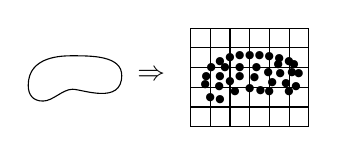
\begin{tikzpicture}[scale=0.25]
  % \draw[step=1.0,black,thin] (-3.,-1.) grid (3,4.);
  % \draw (-3,-1) -- (3,-1) -- (3,4) -- (-3,4) -- (-3,-1);
  \begin{scope}[scale=0.5]
    \draw (-3,0.6) .. controls +(1,0) and +(-1,0) .. (0,1.8)  
    .. controls +(1,0) and +(0,-3) .. (5,3.2) 
    .. controls +(0,2) and +(2,0)  .. (0,5.2) 
    .. controls +(-1,0) and +(0,3) .. (-4.5,2.2) 
    .. controls +(0,-1) and +(-1,0).. (-3,0.6) ;
    \begin{scope}  % pour limiter la portée du clip
      \clip (-3,0.6) .. controls +(1,0) and +(-1,0) .. (0,1.8) 
      .. controls +(1,0) and +(0,-3) .. (5,3.2)
      .. controls +(0,2) and +(2,0)  .. (0,5.2)
      .. controls +(-1,0) and +(0,3) .. (-4.5,2.2)
      .. controls +(0,-1) and +(-1,0).. (-3,0.6);
    \end{scope}
    %\node[below] at (0,1) {$\Omega$};
  \end{scope}
  \node at (4.,1.62) {$\Rightarrow$};
  \begin{scope}[shift={(9,0)}]
    \draw[step=1.0,black,thin] (-3.,-1.) grid (3,4.);
    % contour
    \node at (0,0.9) {\scriptsize$\bullet$}  ;
    \node at (2.5,1.65) {\scriptsize$\bullet$}  ; 
    \node at (0,2.6) {\scriptsize$\bullet$}  ;
    \node at (-2.25,1.1) {\scriptsize$\bullet$}  ; 
    \node at (-1.5,0.35) {\scriptsize$\bullet$}  ; 
    \node at (-2.,0.45) {\scriptsize$\bullet$} ;
    \node at (-2.2,1.5) {\scriptsize$\bullet$}  ; 
    \node at (-1.5,2.3) {\scriptsize$\bullet$} ; 
    \node at (2.35,1.) {\scriptsize$\bullet$}  ;
    \node at (2.25,2.15) {\scriptsize$\bullet$}  ;
    \node at (0.55,0.8) {\scriptsize$\bullet$}  ; 
    \node at (-0.5,2.6) {\scriptsize$\bullet$};
    \node at (0.5,2.59) {\scriptsize$\bullet$}  ;
    \node at (1.5,2.45) {\scriptsize$\bullet$}  ;
    \node at (1,0.75) {\scriptsize$\bullet$}; 
    \node at (2,0.75) {\scriptsize$\bullet$}  ;
    \node at (2,2.3) {\scriptsize$\bullet$}  ;
    \node at (1,2.55) {\scriptsize$\bullet$}  ;
    \node at (-1,2.5) {\scriptsize$\bullet$}  ; 
    \node at (-1.95,2.) {\scriptsize$\bullet$}  ;
    % interior
    \node at (-1.5,1.5) {\scriptsize$\bullet$}  ; 
    \node at (-1.25,2.) {\scriptsize$\bullet$}  ;
    \node at (-0.75,0.75) {\scriptsize$\bullet$}  ; 
    \node at (-1.55,1.){\scriptsize$\bullet$} ;
    \node at (-0.5,1.5) {\scriptsize$\bullet$}  ; 
    \node at (-0.5,2.) {\scriptsize$\bullet$}  ;
    \node at (0.25,1.45) {\scriptsize$\bullet$}  ;
    \node at (0.35,2.) {\scriptsize$\bullet$}  ;
    \node at (0.95,1.75) {\scriptsize$\bullet$}  ;
    \node at (1.15,1.2) {\scriptsize$\bullet$} ;
    \node at (1.45,2.15) {\scriptsize$\bullet$}  ; 
    \node at (1.55,1.65) {\scriptsize$\bullet$}  ;
    \node at (1.85,1.15) {\scriptsize$\bullet$}  ; 
    \node at (2.15,1.75) {\scriptsize$\bullet$}  ;
    \node at (-1.,1.25) {\scriptsize$\bullet$}  ;
    % \draw(3,0.5) -- (3.4,0.5) node [right]  {$\Omega_g$};
  \end{scope}
\end{tikzpicture}

%%% Local Variables:
%%% mode: latex
%%% TeX-master: "../presentation"
%%% End:

  \caption{Discretization of a two-dimensional solid domain using particles in an arbitrary grid.}
  \label{fig:domain}
\end{figure}
The particles are given a mass that enables the definition of the mass density in the grid by recourse to the Dirac delta function:
%In that grid, the reference mass density is described by means of the Dirac delta function and particle masses:
\begin{equation}
  \label{eq:mass_density_DGMPM}
  \rho_0\(\vect{X}\) =  \sum_{p=1}^{N_p} m_p \delta\(\vect{X}^p - \vect{X}\)
\end{equation}
In a similar manner to FEM \cite{Belytschko} and MPM \cite{Sulsky94}, the vector of conserved quantities is approximated on the mesh by:
\begin{equation}
  \label{eq:DGMPM_node2points}
  \Ucb(\vect{X},t) = \sum^{N_n}_{i=1} S_{i}(\vect{X})\Ucb^i(t) 
\end{equation}
with $\Ucb^i$ the vector of conserved quantities at node $i$, and $S_{i}(\vect{X})$ the (linear) shape function attached to it.
Note that particle and nodal quantities are respectively denoted with $p$ and $(i,j)$ subscripts or superscripts.

An approximate solution is sought by means of a weak form that results from multiplication of equation \eqref{eq:conservative_form} by a test function $\Wcb$ and integration over the grid.
According to the Discontinuous Galerkin approximation \cite{NeutronDG,Cockburn}, the test function belongs to a broken polynomial space \cite{DiPietro} in such a way that the weak form is written element-wise.
Thus, after integration by parts, one writes:
\begin{equation}
  \label{eq:DGMPM_weak_form}
  \int_{\Omega^e} \drond{\Ucb}{t} \Wcb \: d\Omega - \int_{\Omega^e} \Fcb_\alpha  \drond{\Wcb}{X_\alpha} \: d\Omega   + \int_{\partial \Omega^e} \Fcb_N  \Wcb \: dS = 0 \quad \forall \: \Wcb,e 
\end{equation}
where $\partial \Omega^e$ is the boundary of the $e$th element with outward normal vector $\vect{N}$.
Boundary integrals then involve interface fluxes $\Fcb_N=\Fcb\cdot \vect{N}$ enabling the propagation of information across cells, the computation of which is presented in section \ref{sec:riemann_solver}.

As for the original MPM \cite{Sulsky94,Sulsky95}, a particle-based quadrature can be used for volume integrals by considering specific fields:
\begin{equation}
  \label{eq:specific_quantities}
  \Ucb = \rho_0 \bar{\Ucb} \quad ; \quad \Fcb_\alpha = \rho_0 \bar{\Fcb}_\alpha
\end{equation}
Indeed, introduction of these fields and the definition of mass density \eqref{eq:mass_density_DGMPM} lead to the following total Lagrangian weak formulation:
\begin{equation} 
  \label{eq:DGMPM_discrete_weak}
  \sum_{p=1}^{N_p} m_p\[\drond{\bar{\Ucb}}{t}  \Wcb - \bar{\Fcb}_{\alpha} \drond{\Wcb}{X_\alpha} \]_{|\vect{X}=\vect{X}^p} + \int_{\partial \Omega^e} \Fcb_N  \Wcb \: dS = 0 \quad \forall \: \Wcb,e
\end{equation}

At last, the semi-discrete system is written by introducing the DGMPM approximation \eqref{eq:DGMPM_node2points} and considering the arbitrariness of the test function:
\begin{equation}
  \label{eq:DGMPM_semi_discrete}
  \sum_{p=1}^{N_p}\[ S_{ip} m_p S_{jp} \drond{\bar{\Ucb}^j}{t}  - \drond{S_{ip}}{X_\alpha} m_p S_{jp} \bar{\Fcb}^j_{\alpha} \] + \int_{\partial \Omega^e} S_i(\vect{X}) \Fcb_N  \: dS =  0  \quad \forall \: e
\end{equation}
or, in matrix form:
\begin{equation}
  \label{eq:DGMPM_semi_discrete_matrix}
  M_{ij} \drond{\bar{\Ucb}^j}{t} - K^\alpha_{ij} \bar{\Fcb}^j_{\alpha} + \vect{\hat{\Fc}}^i = \vect{0}  
\end{equation}
Note however that the particle-based quadrature may lead to a singular consistent mass matrix due to enventual reduced integrations \cite{Love}.
This issue can be circumvented by using the diagonally lumped mass matrix $M^L_i=\sum_j M_{ij}$.

The discrete system is derived by discretizing the time interval $\tau$ into $N_t$ subintervals and using the explicit forward Euler method:
\begin{equation}
  \label{eq:DGMPM_discrete}
  M^L_i \frac{\bar{\Ucb}^{i,n+1} - \bar{\Ucb}^{i,n}}{\Delta t^{n} } = K^\alpha_{ij} \bar{\Fcb}_{\alpha}^{j,n} - \vect{\hat{\Fc}}^{i,n}  
\end{equation}
where the superscripts $(\bullet)^{k,l}$ denote a field evaluated at node $k$ and time step $l$.
% \review{Alternatively, a \textit{second-order Runge-Kutta (RK2)} explicit time discretization may be employed, leading to the following two-stage discrete form:
% \begin{equation}
%   \label{eq:DGMPM_discrete_RK2}
%   \begin{aligned}
%     & M^L_i \frac{\bar{\Ucb}^{i,n+1/2} - \bar{\Ucb}^{i,n}}{\Delta t^{n} } = \frac{1}{2}\(K^\alpha_{ij} \bar{\Fcb}_{\alpha}^{j,n} - \vect{\hat{\Fc}}^{i,n}\)  \\
%     & M^L_i \frac{\bar{\Ucb}^{i,n+1} - \bar{\Ucb}^{i,n}}{\Delta t^{n} } = K^\alpha_{ij} \bar{\Fcb}_{\alpha}^{j,n+1/2} - \vect{\hat{\Fc}}^{i,n+1/2}
%   \end{aligned}
% \end{equation}
% \textit{
%   We chose here one existing two-stage second order Runge-Kutta method among others. See for instance \cite{Leveque} for a Total Variation Diminishing version of the RK2 time discretization. 
% }}

As for MPM, a discrete system is solved at nodes while the loading history is stored at material points.
Hence, a reconstruction of fields on the grid based on particle values is required as well as a projection of the updated solution from the grid to the material points.
The reconstruction procedure is similar to that used within the MPM and consists in ensuring the conservation of volume quantities:
\begin{equation}
  \label{eq:reconstruction}
  \bar{\Ucb}^{i,n} =  \frac{\sum_{p=1}^{N_p}S_{ip}m_p\bar{\Ucb}^{p,n}}{M_{i}^L }  \quad \text{for } i=1,...,N_n
\end{equation}
The back-mapping follows that proposed in the Particle-In-Cell method (PIC) \cite{PIC}, namely, a classical interpolation:
\begin{equation}
  \label{eq:back_mapping}
  \bar{\Ucb}^{p,n+1}=\sum_{i=1}^{N_n} S_{ip}\bar{\Ucb}^{i,n+1}
\end{equation}
Notice that the MPM is based on a different projection from nodes to particles that was introduced in the FLuid Implicit Particle method (FLIP) \cite{Mass_Flip}.
The FLIP mapping reduces the numerical diffusion resulting from the interpolation used in PIC at the cost of spurious oscillations.
The employment of the PIC projection rather than the FLIP one within the DGMPM is motivated by the willingness to avoid oscillations that can, for plastic materials, lead to a premature plastic flow due to overshoots in the stress values.
On the other hand, the diffusion inherent in PIC mapping is expected to be less significant with discontinuous shape functions due to the reduction of the domain of influence of nodes.

\subsection{Intercell fluxes}
%% Elastoplastic approximate Riemann solver for one-dimensional problems
%% Elastic Riemann solver + variational solver for multi-dimensional
\label{sec:riemann_solver}
% \begin{theorem}[Godunov \cite{Godunov_method}]
%   \label{th:Godunov}
%   Monotone linear numerical schemes can be at most first-order accurate.
% \end{theorem}

DG methods for hyperbolic problems are based on the requirement of ensuring monotonicity of the scheme for piecewise constant approximations \cite{Cockburn}. 
Such a numerical method is monotone for flux functions $\Fcb_N$ that are Lipschitz continuous, consistent and monotone, namely, they must be \textit{E-fluxes} \cite{Osher}.
One possibility, which is widely used and adopted here, is the \textit{Godunov flux function}. 

Let's consider the following Riemann problem that can be defined at the interface between two DGMPM cells having normal vector $\vect{N}$:
\begin{equation}
  \label{eq:RP_mesh}
  \begin{aligned}
    &\drond{\Ucb}{t} + \drond{\Fcb_N}{X_N} = \vect{0}  \\
    & \Ucb(X_N,0)= \left\lbrace 
      \begin{aligned}
        & \Ucb_{X_N^-} \text{ if } X_N < 0 \\
        & \Ucb_{X_N^{+}} \text{ if } X_N > 0
      \end{aligned}
        \right.
  \end{aligned}
\end{equation}
The intitial conditions $\Ucb_{X_N^-}$ and $\Ucb_{X_N^{+}}$ result from the average of nodal fields on each side of the interface, so that one Riemann problem is solved at each edge (see a two-dimensional example in figure \ref{fig:2D_edge}).

 
\begin{figure}[ht]
  \centering
  \begin{tikzpicture}[scale=0.5]
  \draw (10.,0.) -- (12.,6.) ; 
  \draw[fill=black] (9.85,0.1) circle (0.1) node [left] {$1$};	
  \draw[fill=black] (10.2,-0.0) circle (0.1) node [right] {$2$};	
  \draw[fill=black] (11.85,6.1) circle (0.1) node [left] {$4$};	
  \draw[fill=black] (12.2,6) circle (0.1) node [right] {$3$};	
  \draw[->,very thick] (11.,3.) -- (12,3 -1/3) node [right,below] {$X_N$}; 
  \node at (8,3.5) {$\vect{\Qc}_{L} = \frac{\vect{\Qc}_1 + \vect{\Qc}_4}{2}$}; \node at (14.5,3.5) {$\vect{\Qc}_{R} = \frac{\vect{\Qc}_2 + \vect{\Qc}_3}{2}$};
\end{tikzpicture}

  \caption{Duplication of nodes at an interface and building of initial conditions of the Riemann problem (2D).}
  \label{fig:2D_edge}
\end{figure}
The characteristic structure of the solution of problem \eqref{eq:RP_mesh} consists of waves emanating from the origin of the $(X_N,t)$ plane \cite{Courant}.
The wave pattern can be determined by the spectral analysis of the Jacobian matrix: $\Jbsf_\Uc = \drond{\Fcb_N}{\Ucb}$.
The eigenvalues $c_k$ and associated right eigenvectors $\Rcb^k$ ($k=1, ..., D$), $D$ being the dimension of the Jacobian, are respectively stored as diagonal entries and columns of matrices $\Cbsf$ and $\Rbsf$ which are defined as:
\begin{equation}
  \label{eq:eigen_matrices}
  \Jbsf_\Uc \Rbsf = \Rbsf \Cbsf
\end{equation}
% For flux vectors that are non-linear functions of $\Ucb$, as those involved for hyperelastic constitutive models, simple and shock waves may occur \cite{Wang} so that solving the problem drastically increases the computational cost.
For flux vectors that are non-linear functions of $\Ucb$, as those involved for hyperelastic constitutive models, solving problem \eqref{eq:RP_mesh} drastically increases the computational cost since this requires iterative procedures.
Nonetheless, linearized Riemann solvers \cite{Toro} can be constructed by approximating $\Jbsf_\Uc$ in the vicinity of $\Ucb_{X_N^-}$ and $\Ucb_{X_N^+}$ by a constant matrix $\underline{\Jbsf}(\Ucb_{X_N^-},\Ucb_{X_N^+})$.
The matrix $\underline{\Jbsf}$ must however ensure the hyperbolicity, namely $\underline{\Jbsf}$ has real eigenvalues and a complete set of independent eigenvectors \cite{Courant}, and satisfy the consistency condition \cite{Leveque}:
\begin{equation}
  \label{eq:consistency_Jacobian}
  \underline{\Jbsf}(\Ucb,\Ucb) = \Jbsf_\Ucb(\Ucb) 
\end{equation}
Both conditions can be satisfied by assuming that the negative (\textit{resp. positive}) eigenvalues and the associated right eigenvectors of $\Jbsf_\Ucb$, which correspond to left-going (\textit{resp. right-going}) waves, depend only on  $\Ucb_{X_N^-}$ (\textit{resp. on $\Ucb_{X_N^+}$}).
Then, defining the matrices:
\begin{align*}
  &\underline{\Cbsf}=\matrice{c_1(\Ucb_{X_N^-}) & & & & & \\ & \cdots & & && \\ & &c_I(\Ucb_{X_N^-}) & & &\\ & & &c_{I+1}(\Ucb_{X_N^+})& & \\ & & & &\cdots &\\ &&&&&c_D(\Ucb_{X_N^+})} \\
  &\underline{\Rbsf} = \matrice{\Rcb^1(\Ucb_{X_N^-}),\:  ...\:  ,\: \Rcb^I(\Ucb_{X_N^-}),\: \Rcb^{I+1}(\Ucb_{X_N^+}),\:...\: ,\: \Rcb^D(\Ucb_{X_N^+})} 
\end{align*}
in which $c_1<\cdots <c_I<c_{I+1}<\cdots < c_D$, the following approximation fulfills the requirements provided that $\Jcb_\Uc$ ensures the hyperbolicity:
\begin{equation}
  \label{eq:3}
  \underline{\Jbsf} = \underline{\Rbsf} \: \underline{\Cbsf} \: \underline{\Rbsf}^{-1}
\end{equation}

Though approximate-flux Riemann solvers, which extract information for flux functions, have been applied to hyper solids (see Osher's solver in \cite{Haider_FVM,Lee_FVM} or the HLLC solver in \cite{Ortega_HLLD}), the approximate-state Riemann solver is considered here.
The procedure then consists in computing the stationary solution of the linearized Riemann problem as \cite{Toro}:
\begin{equation}
  \label{eq:stationary_solution}
  \Ucb^* = \Ucb_{X_N^-} + \sum_{\underset{c_k < 0}{k=1}}^D \delta_k\Rcb^k = \Ucb_{X_N^+} - \sum_{\underset{c_k > 0}{k=1}}^D \delta_k\Rcb^k
\end{equation}
where the $\delta_k$ are wave strength coefficients related to the $k$th wave of the characteristic structure.
These coefficients can be computed by rearranging equation \eqref{eq:stationary_solution} as:
\begin{equation}
  \label{eq:delta_U}
  \Ucb_{X_N^+} - \Ucb_{X_N^-} = \sum_{k=1}^D \delta_k\Rcb^k
\end{equation}
so as to compute the stationary solution.
Once $\Ucb^*$ is known, the intercell flux is computed as $\Fcb_N\(\Ucb^*\)$ according to Godunov's method \cite{Godunov_method}.
Since the vector of conserved quantities $\Ucb$ contains the deformation gradient and the linear momentum while the flux is composed of stress and velocity, the integration of constitutive equations, which may be costly, is required. 
This can however be avoided by formulating the Riemann problem based on the quasi-linear form \eqref{eq:quasi-linear} involving velocity and stress, thus allowing the direct computation of intercell fluxes through the auxiliary vector $\Qcb$.
This approch then requires that stress as well as velocity and strain are projected from the material points to the nodes by means of the reconstruction \eqref{eq:reconstruction}.

% \begin{remark}
% Hyperbolic systems having zero eigenvalues lead to stationary waves, propagating at zero celerity, across which the solution of the Riemann problem may have discontinuities.
%   In that case, the associated Godunov flux is also discontinuous so that one stationary state must be considered on both sides of the characteristic.
%   This approach leads to the computation of two fluxes, each contributing to one cell only. 
% \end{remark}

\begin{remark}
  The approximate-state Riemann solver described above allows to account for the transverse propagation of waves by adding correction terms on the intercell fluxes similarly similarly to the Corner Transport Upwind method (CTU) \cite{Colella_CTU}.
  The use of the CTU within the DGMPM, presented in \cite{DGMPM}, enables the improvement of the stability properties of the scheme for problems involving Poisson's effect \cite{Thesis}.
\end{remark}


As seen in section \ref{sec:continuum_problem}, the Jacobian matrix of the system involves the fourth-order tangent modulus tensor.
However, this tensor is responsible for a more complex characteristic structure when plastic flow occurs since one has to take into account both elastic and plastic waves in that case \cite{Wang}.
For small strain problems, the corresponding characteristic structure is known in particular cases so that dedicated Riemann solvers have been developed for one-dimensional media \cite{Thomas_EP} or for combined longitudinal and torsional stress loadings \cite{Lin_et_Ballman}.
Given the complexity introduced by finite deformations, such solvers cannot be considered.
As a result, a purely reversible evolution is commonly considered for the computation of intercell fluxes, followed by the integration of the plastic flow by using a return mapping algorithm in finite volume simulations (see \cite{FRRSE,Maire_elastoplast} for hypoelastic-plastic materials and \cite{Lee_FVM} for hyperelastic-plastic ones).
A similar approach is adopted here in such a way that the DGMPM scheme consists in a predictor-corrector procedure, the integration of plastic flow being carried out through variational constitutive updates.
This is the object of the next section.



%%% Local Variables:
%%% mode: latex
%%% TeX-master: "manuscript"
%%% End:


\section{Computation of intercell fluxes}
\label{sec:riemann_solver}
%\subsection{Intercell fluxes}
%% Elastoplastic approximate Riemann solver for one-dimensional problems
%% Elastic Riemann solver + variational solver for multi-dimensional
DG methods for hyperbolic problems are based on the requirement of ensuring monotonicity of the scheme for piecewise constant approximations \cite{Cockburn}. 
Such approaches are monotone for flux functions $\Fcb_N$ that are Lipschitz continuous, consistent and monotone, namely, they must be E-fluxes \cite{Osher}.
One possibility, which is widely used and adopted here, is the Godunov flux function. 

Let's consider the following Riemann problem defined at the interface between two DGMPM cells having normal vector $\vect{N}$:
\begin{equation}
  \label{eq:RP_mesh}
  \begin{aligned}
    &\drond{\Ucb}{t} + \drond{\Fcb_N}{X_N} = \vect{0}, \quad X_N=\vect{X}\cdot\vect{N}  \\
    & \Ucb(X_N,0)= \left\lbrace 
      \begin{aligned}
        & \Ucb_{X_N^-} \text{ if } X_N < 0 \\
        & \Ucb_{X_N^{+}} \text{ if } X_N > 0
      \end{aligned}
        \right.
  \end{aligned}
\end{equation}
The initial conditions $\Ucb_{X_N^-}$ and $\Ucb_{X_N^{+}}$ result from the average of nodal fields on each side of the interface, so that one Riemann problem is solved at each edge (see a two-dimensional example in figure \ref{fig:2D_edge}).

 
\begin{figure}[ht]
  \centering
  \begin{tikzpicture}[scale=0.5]
  \draw (10.,0.) -- (12.,6.) ; 
  \draw[fill=black] (9.85,0.1) circle (0.1) node [left] {$1$};	
  \draw[fill=black] (10.2,-0.0) circle (0.1) node [right] {$2$};	
  \draw[fill=black] (11.85,6.1) circle (0.1) node [left] {$4$};	
  \draw[fill=black] (12.2,6) circle (0.1) node [right] {$3$};	
  \draw[->,very thick] (11.,3.) -- (12,3 -1/3) node [right,below] {$X_N$}; 
  \node at (8,3.5) {$\vect{\Qc}_{L} = \frac{\vect{\Qc}_1 + \vect{\Qc}_4}{2}$}; \node at (14.5,3.5) {$\vect{\Qc}_{R} = \frac{\vect{\Qc}_2 + \vect{\Qc}_3}{2}$};
\end{tikzpicture}

  \caption{Duplication of nodes at an interface and building of initial conditions of the Riemann problem (2D).}
  \label{fig:2D_edge}
\end{figure}
The characteristic structure of the solution of problem \eqref{eq:RP_mesh} consists of waves emanating from the origin of the $(X_N,t)$ plane \cite{Courant}.
The wave pattern can be determined by the spectral analysis of the Jacobian matrix: $\Jbsf_\Uc = \drond{\Fcb_N}{\Ucb}$.
The eigenvalues $c_k$ and associated right eigenvectors $\Rcb^k$ ($k=1, ..., D$), $D$ being the dimension of the Jacobian, are respectively stored as diagonal entries and columns of matrices $\Cbsf$ and $\Rbsf$ which are defined as:
\begin{equation}
  \label{eq:eigen_matrices}
  \Jbsf_\Uc \Rbsf = \Rbsf \Cbsf
\end{equation}
For flux vectors that are non-linear functions of $\Ucb$, as those involved for hyperelastic constitutive models, solving problem \eqref{eq:RP_mesh} drastically increases the computational cost since this requires iterative procedures.
Nonetheless, linearized Riemann solvers \cite{Toro} can be constructed by approximating $\Jbsf_\Uc$ in the vicinity of $\Ucb_{X_N^-}$ and $\Ucb_{X_N^+}$ by a constant matrix $\underline{\Jbsf}(\Ucb_{X_N^-},\Ucb_{X_N^+})$.
The matrix $\underline{\Jbsf}$ must however ensure the hyperbolicity, namely $\underline{\Jbsf}$ has real eigenvalues and a complete set of independent eigenvectors \cite{Courant}, and satisfy the consistency condition \cite{Leveque}:
\begin{equation}
  \label{eq:consistency_Jacobian}
  \underline{\Jbsf}(\Ucb,\Ucb) = \Jbsf_\Ucb(\Ucb) 
\end{equation}
Both conditions can be satisfied by assuming that the negative (\textit{resp. positive}) eigenvalues and the associated right eigenvectors of $\Jbsf_\Ucb$, which correspond to left-going (\textit{resp. right-going}) waves, depend only on  $\Ucb_{X_N^-}$ (\textit{resp. on $\Ucb_{X_N^+}$}).
Then, defining the matrices:
\begin{align*}
  &\underline{\Cbsf}=\matrice{c_1(\Ucb_{X_N^-}) & & & & & \\ & \cdots & & && \\ & &c_I(\Ucb_{X_N^-}) & & &\\ & & &c_{I+1}(\Ucb_{X_N^+})& & \\ & & & &\cdots &\\ &&&&&c_D(\Ucb_{X_N^+})} \\
  &\underline{\Rbsf} = \matrice{\Rcb^1(\Ucb_{X_N^-}),\:  ...\:  ,\: \Rcb^I(\Ucb_{X_N^-}),\: \Rcb^{I+1}(\Ucb_{X_N^+}),\:...\: ,\: \Rcb^D(\Ucb_{X_N^+})} 
\end{align*}
in which $c_1<\cdots <c_I<c_{I+1}<\cdots < c_D$, the following approximation fulfills the requirements provided that $\Jbsf_\Uc$ ensures the hyperbolicity:
\begin{equation}
  \label{eq:3}
  \underline{\Jbsf} = \underline{\Rbsf} \: \underline{\Cbsf} \: \underline{\Rbsf}^{-1}
\end{equation}

Though approximate-flux Riemann solvers, which extract information for flux functions, have been applied to hyperelastic solids (see Osher's solver in \cite{Haider_FVM,Lee_FVM} or the HLLC solver in \cite{Ortega_HLLD}), the approximate-state Riemann solver is considered here.
The procedure then consists in computing the stationary solution of the linearized Riemann problem as \cite{Toro}:
\begin{equation}
  \label{eq:stationary_solution}
  \Ucb^* = \Ucb_{X_N^-} + \sum_{\underset{c_k < 0}{k=1}}^D \delta_k\Rcb^k = \Ucb_{X_N^+} - \sum_{\underset{c_k > 0}{k=1}}^D \delta_k\Rcb^k
\end{equation}
where the $\delta_k$ are wave strength coefficients related to the $k$th wave of the characteristic structure.
These coefficients can be computed by rearranging equation \eqref{eq:stationary_solution} as:
\begin{equation}
  \label{eq:delta_U}
  \Ucb_{X_N^+} - \Ucb_{X_N^-} = \sum_{k=1}^D \delta_k\Rcb^k
\end{equation}
so as to compute the stationary solution.
Once $\Ucb^*$ is known, the intercell flux is computed as $\Fcb_N\(\Ucb^*\)$ according to Godunov's method \cite{Godunov_method}.
Since the vector of conserved quantities $\Ucb$ contains the deformation gradient and the linear momentum while the flux consists of the stress and the velocity, the integration of constitutive equations is needed, which may be costly.
This can however be avoided by solving the Riemann problem based on the quasi-linear form \eqref{eq:quasi-linear}, which involves the velocity and the stress.
Thus, an approximate-state Riemann solver can be built upon the linearized Jacobian matrix related to the quasi-linear form:
\begin{equation}
  \label{eq:jacobian_quasi}
  \underline{\Jbsf}_\Qcb = \underline{\Rbsf}_\Qcb \: \underline{\Cbsf} \: \underline{\Rbsf}_\Qcb^{-1}
\end{equation}
where $\underline{\Rbsf}_\Qcb$ is the approximate matrix of the right eigenvectors of the Jacobian matrix associated with the quasi-linear form.
Then, the stationary solution of the Riemann problem reads:
\begin{equation}
  \label{eq:stationary_solution_Q}
  \Qcb^* = \Qcb_{X_N^-} + \sum_{\underset{c_k < 0}{k=1}}^D \delta_k\Rcb_\Qcb^k = \Qcb_{X_N^+} - \sum_{\underset{c_k > 0}{k=1}}^D \delta_k\Rcb_\Qcb^k
\end{equation}
in which the wave strength coefficients can be computed as:
\begin{equation}
  \label{eq:delta_U}
  \Qcb_{X_N^+} - \Qcb_{X_N^-} = \sum_{k=1}^D \delta_k\Rcb_\Qcb^k
\end{equation}
Therefore, the auxiliary stationary state $\Qcb^*$ enables the direct calculation of intercell fluxes.
Notice however that this approach requires the projection of the velocity and the strain along with the stress from the material points to the nodes by means of the reconstruction \eqref{eq:reconstruction}.


\begin{remark}
  Intercell fluxes can also account for the transverse propagation of waves by adding correction terms similar to these of the Corner Transport Upwind method (CTU) \cite{Colella_CTU}.
  The use of the CTU within the DGMPM has been presented in \cite{DGMPM} and enables the improvement of the stability properties of the scheme for problems involving Poisson's effect \cite{Thesis}.
\end{remark}


As seen in section \ref{sec:continuum_problem}, the fourth-order tangent modulus tensor arises in the Jacobian matrix of the quasi-linear form.
This tensor is responsible for a more complex characteristic structure when plastic flow occurs since one has to take into account both elastic and plastic waves.
For small strain problems, the corresponding characteristic structure is known in particular cases so that dedicated Riemann solvers have been developed for one-dimensional media \cite{Thomas_EP} or for combined longitudinal and torsional stress loadings \cite{Lin_et_Ballman}.
Given the mathematical complexity introduced by large strains, such solvers cannot be considered for finite deforming solids so far.
As a result, a purely reversible evolution is commonly considered for the computation of intercell fluxes, followed by the integration of the plastic flow by using a return mapping algorithm in finite volume simulations (see \cite{FRRSE,Maire_elastoplast} for hypoelastic-plastic materials and \cite{Lee_FVM} for hyperelastic-plastic ones).
A similar approach is adopted here in such a way that the DGMPM scheme consists in a predictor-corrector procedure, the integration of plastic flow being carried out through variational constitutive updates.
This is the object of the next section.


%%% Local Variables:
%%% mode: latex
%%% TeX-master: "manuscript"
%%% End:


\section{Variational constitutive update}
\label{sec:constitutive-update}

%The variational reformulation of the constitutive equations derived in section \ref{subsec:cont_constitutive} is carried out by introducing the following power density function \cite{Laurent2010}:
%The variational formulation of the constitutive relations derived in section \ref{subsec:cont_constitutive} follows from the minimization of the power density function \cite{Laurent99,Laurent2010}:
% Let's introduce the following power density function \cite{Laurent2010}:
The constitutive equations derived in section  \ref{subsec:cont_constitutive}, which account for the dependence of the material on the loading history, are usually integrated within an incremental procedure by means of radial return algorithms \cite{Simo}. 
Alternatively, the set of equations can be formulated as an optimization problem by introducing some power density function \cite{Laurent99,Laurent2010}:
\begin{equation}
  \label{eq:rate_potential}
  \Pscr(\tens{\dot{F}},\dot{\Vcb}) = \drond{\psi}{\tens{F}}:\tens{\dot{F}} - \Acb\cdot \dot{\Vcb} + \phi^*(\dot{\Vcb})
\end{equation}
whose minimizations with respect to $\dot{\Vcb}$ and $\tens{M}$ respectively lead to:
\begin{equation}
  \label{eq:optimization}
  -\Acb + \drond{\phi^*}{\dot{\Vcb}} = 0  \quad ;\quad \underset{\tens{M}}{\max} \left\lbrace \tens{T}\(\tens{M}\tens{F}^p\) \cdot \dot{\Vcb}\right\rbrace
\end{equation}
The first equation is the dual form of the kinetic equations \eqref{eq:dual_form_kinetic} while the second one yields the determination of the plastic flow direction by satisfying the principle of maximum plastic dissipation.
Moreover, it can  be shown that the effective power density $\Pscr^{eff}(\tens{\dot{F}})= \underset{\dot{\Vcb},\tens{M}}{\min} \: \Pscr$
% \begin{equation}
%   \label{eq:effective_power_density}
%   \Pscr^{eff}(\tens{\dot{F}})= \underset{\dot{\Vcb},\tens{M}}{\min} \: \Pscr
% \end{equation}
acts as a rate potential for $\tens{\Pi}$, that is:
\begin{equation}
  \label{eq:PK1_rate_potential}
  \tens{\Pi}=\drond{\Pscr^{eff}}{\tens{\dot{F}}}
\end{equation}

Variational constitutive updates can be constructed upon approximations of $\Pscr^{eff}$ by introducing the incremental energy function:
\begin{equation}
  \label{eq:incremental_energy}
  W(\tens{F}_{n+1};\tens{F}_n,\Vcb_n) = \underset{\Vcb_{n+1},\tens{M}}{\min} \:\left\lbrace \psi\(\tens{F}_{n+1},\tens{F}^p_{n+1},\Vcb_{n+1}\) -\psi\(\tens{F}_{n},\tens{F}^p_{n},\Vcb_{n}\) + \Delta t \left\langle \phi^*\(\dot{\Vcb}_{n}\)\right\rangle\right\rbrace
\end{equation}
In equation \eqref{eq:incremental_energy}, it is understood that the subscripts refer to time increments and that the thermodynamic state $(\tens{F}_n,\tens{F}^p_n,\Vcb_n)$, as well as the updated deformation gradient $\tens{F}_{n+1}$, are known.
Thus, the plastic part of the deformation gradient results from the incremental plastic flow rule: 
\begin{equation}
  \label{eq:flow_rule_inc}
  \tens{F}^p_{n+1}=\exp \(\Delta \Vcb \tens{M} \)\tens{F}^p_n
\end{equation}
in which $\Delta \Vcb = \Vcb_{n+1}-\Vcb_n$, and $\tens{M}$ and $\Vcb_{n+1}$ are the argument of the optimization \eqref{eq:incremental_energy}.
At last, the updated first Piola-Kirchhoff stress tensor is:
\begin{equation}
  \label{eq:PK1_inc}
  \tens{\Pi}_{n+1} = \left.\drond{\psi}{\tens{F}}\right|_{t_{n+1}}=\drond{W(\tens{F}_{n+1})}{\tens{F}_{n+1}}
\end{equation}
so that $W$ appears as a potential for $\tens{\Pi}_{n+1}$.

%\review{Comments needed here about the advantages of such approaches}



%%% Local Variables:
%%% mode: latex
%%% TeX-master: "manuscript"
%%% End:


\section{Numerical results}
\label{sec:test_cases}
Although some properties of the simple waves have been given in section \ref{sec:stress_paths}, the complexity of the equations prevents the complete characterization of the loading paths followed.
In order to get additional information about the evolution of the stress states within, the systems of ODEs gathered in table \ref{tab:simpleWavesEquations} are numerically integrated in this section for plane stress and plane strain loadings, based on the material parameters used in chapter \ref{chap:chap3}.
In particular, the thin-walled tube problem considered by Clifton \cite{Clifton} is first looked at so that the above developments can be validated.
Next, the plane stress and plane strain cases are treated.
The identified behaviors should provide some simplification assumptions for the building of a procedure that lead to approximate solutions of the problems.
The values of the elastic properties considered here are those use in the previous chapter (see table \ref{tab:material}).
On the other hand, the tensile yield stress $\sigma^y=10^{8} \: Pa$ and the hardening modulus $C=1\times10^8 \: Pa$ are set here arbitrarily.
Finally, we restrict here to positive shear stress $\sigma_{12}\geq 0$.
\subsection{Thin-walled tube problem}
%% Hypothèses du problème
Consider the semi-infinite domain in Cartesian coordinate system: $x_1 \times x_2 \times x_3 \in [0,\infty[ \times ]-\infty,\infty[ \times [-\infty,\infty]$, being acted upon by a traction vector $\vect{T}^d$ at $x_1=0 $.
Only the first two components of $\vect{T}^d$ are non-null so that the stress and strain tensor within the medium are of the form:
\begin{equation}
  \tens{\sigma} = \matrice{\sigma_{11} & \sigma_{12} & \\ \sigma_{12} & 0 & \\ & & 0} \quad ;\quad\tens{\eps} = \matrice{\eps_{11} & \eps_{12} & \\ \eps_{12} & \eps_{22}& \\ & & \eps_{33}}
\end{equation}
Such a state corresponds to that holding in a hollow cylinder with radius and length much bigger that its thickness, submitted to combined longitudinal and torsional loads.
Hence the name of thin-walled tube problem. 
As a particular plane stress case, the set of ODEs along characteristic derived in section \ref{sec:stress_paths} applies with nevertheless, taking into account the vanishing stress component $\sigma_{22}$.
Indeed, for plane stress one has:
\begin{equation*}
  \dot{\sigma}_{22}=\widetilde{C}^{ep}_{22ij} \dot{\eps}_{ij} =0 \quad i,j=\{1,2\}
\end{equation*}
where $\widetilde{\Cbb}^{ep}$ is the plane stress tangent modulus \eqref{eq:CP_constitutive}.
\begin{equation*}
  \widetilde{C}^{ep}_{2222} \dot{\eps}_{22} = - \widetilde{C}^{ep}_{22ij}\dot{\eps}_{ij} \quad ij=\{11,12,21\}
\end{equation*}
Thus, inverting the above equation and introducing it in the constitutive equation, we are left with the following law:
\begin{equation}
  \label{eq:ch5_TW_tangent}
  \dot{\sigma}_{ij}=\widetilde{C}^{ep}_{ijkl} \dot{\eps}_{kl} - \frac{\widetilde{C}^{ep}_{ij22}\widetilde{C}^{ep}_{22kl}}{\widetilde{C}^{ep}_{2222}}\dot{\eps}_{kl}= \widehat{C}^{ep}_{ijkl} \dot{\eps}_{kl}\qquad ij,kl=\{11,12,21\} 
\end{equation}
where $\widetilde{\Cbb}^{ep}$ is referred to as the thin-walled tube tangent modulus.
The characteristic analysis of the hyperbolic system based on this tangent modulus also leads to loading paths followed across slow and fast waves, involving nevertheless two components of stress only. For the sake of simplicity, the stress components are denoted by $\sigma_{11}=\sigma$ and $\sigma_{12}=\tau$ whereas the velocity components reads $v_1=u$ and $v_2=v$ in what follows.

Those equations as well as these of Clifton \cite{Clifton} have been numerically integrated numerically, starting from several points lying on the initial yield surface.
The loading functions are odd functions of $\sigma$ and $\tau$ \cite{Clifton} so that the loading paths have axial symmetries.
Hence, the study is restricted to the quarter-plane $\sigma>0,\tau>0$.

\begin{figure}[h!]
  \centering
  \subcaptionbox{Stress path in $(\sigma,\tau)$ plane \label{subfig:tw_fast_stress}}{\begin{tikzpicture}[scale=0.9]
  \begin{axis}[ymajorgrids=true,xmajorgrids=true,ylabel=$\tau \: (Pa)$,xlabel=$\sigma \: (Pa)$,legend style={legend pos=south west}]
    %%
    \addplot[Blue,mark=x,only marks,mark repeat=10,very thick,mark size=3pt] table [x=sigma_11,y=sigma_12] {chapter5/pgfFigures/pgf_thinWalledTubeFastWave/fastStressPlane_Stress.pgf};
    \addlegendentry{Present work}
    \addplot[arrows along my path,Red,thick] table [x=sigma_11,y=sigma_12] {chapter5/pgfFigures/pgf_thinWalledTubeFastWave/TWfastStressPlane_Stress.pgf};
    \addlegendentry{Clifton}
    %% Yield surface
    \addplot[black,dashed] table  [x=sigma_11,y=sigma_12] {chapter5/pgfFigures/pgf_thinWalledTubeSlowWave/TWslow_yield0.pgf};
    \addlegendentry{initial yield surface}
  \end{axis}
\end{tikzpicture}

%%% Local Variables:
%%% mode: latex
%%% TeX-master: "../../mainManuscript"
%%% End:} \qquad
  \subcaptionbox{Stress path in deviatoric plane\label{subfig:tw_fast_dev}}{\tikzset{cross/.style={cross out, draw=black, minimum size=2*(#1-\pgflinewidth), inner sep=0pt, outer sep=0pt},
%default radius will be 1pt. 
cross/.default={2.5pt}}
\begin{tikzpicture}[scale=0.8]
  \begin{axis}[width=.75\textwidth,view={135}{35.2643},xlabel=$s_1 $,
    ylabel=$s_2 $,zlabel=$s_3$,xmin=-1.e8,xmax=1.e8,ymin=-1.e8,ymax=1.e8,axis equal,axis lines=center,axis on top,xtick=\empty,ytick=\empty,ztick=\empty,
    every axis y label/.style={at={(rel axis cs:0.,.5,-0.65)}, anchor=west},
    every axis x label/.style={at={(rel axis cs:0.5,.,-0.65)}, anchor=east},
    every axis z label/.style={at={(rel axis cs:0.,.0,.18)}, anchor=north},
    legend style={at={(1.125,.59)}}
    ]
    \node[below] at (axis cs:1.1e8,0.,0.) {$\sigma^y$};
    \node[above] at (axis cs:-1.1e8,0.,0.) {$-\sigma^y$};
    \draw (axis cs:1.e8,0.,0.) node[cross,rotate=10] {};
    \draw (axis cs:-1.e8,0.,0.) node[cross,rotate=10] {};
    \node[white]  at (axis cs:0,0.,1.42e8) {};
    %%
    \addplot3[black,mark=x,only marks,mark repeat=20,thick,mark size=3pt] file {section7/pgfFigures/pgf_thinWalledTubeFastWave/TWfastDevPlane_Stress.pgf};
    \addplot3[black,arrows along my path,thick] file {section7/pgfFigures/pgf_thinWalledTubeFastWave/fastDevPlane_Stress.pgf};
    \addlegendentry{Clifton}
    \addlegendentry{This work}
    %% Yield surface
    \addplot3[black,dashed] file {section7/pgfFigures/pgf_thinWalledTubeSlowWave/TWCylindreDevPlane.pgf};
    \addlegendentry{Initial yield surface}
    \newcommand\radius{0.82e8}
    \addplot3[dotted,thick] coordinates {(0.75*\radius,-0.75*\radius,0.) (-0.75*\radius,0.75*\radius,0.)};
    \addplot3[dotted,thick] coordinates {(0.,-0.75*\radius,0.75*\radius) (0.,0.75*\radius,-0.75*\radius)};
    \addplot3[dotted,thick] coordinates {(-0.75*\radius,0.,0.75*\radius) (0.75*\radius,0.,-0.75*\radius)};

  \end{axis}
  \begin{scope}[shift={(8.5,0.)}]
    \begin{axis}[width=.75\textwidth,view={135}{35.2643},xlabel=$s_1 $,
    ylabel=$s_2 $,zlabel=$s_3$,xmin=-1.e8,xmax=1.e8,ymin=-1.e8,ymax=1.e8,axis equal,axis lines=center,axis on top,xtick=\empty,ytick=\empty,ztick=\empty,
    every axis y label/.style={at={(rel axis cs:0.,.5,-0.65)}, anchor=west},
    every axis x label/.style={at={(rel axis cs:0.5,.,-0.65)}, anchor=east},
    every axis z label/.style={at={(rel axis cs:0.,.0,.18)}, anchor=north}
    ]
    \node[below] at (axis cs:1.1e8,0.,0.) {$\sigma^y$};
    \node[above] at (axis cs:-1.1e8,0.,0.) {$-\sigma^y$};
    \draw (axis cs:1.e8,0.,0.) node[cross,rotate=10] {};
    \draw (axis cs:-1.e8,0.,0.) node[cross,rotate=10] {};
    \node[white]  at (axis cs:0,0.,1.42e8) {};
    %%
    \addplot3[black,mark=x,only marks,mark repeat=30,thick] file {section7/pgfFigures/pgf_thinWalledTubeSlowWave/TWslowDevPlane_Stress0.pgf};
    \addplot3[black,arrows along my path,thick] file {section7/pgfFigures/pgf_thinWalledTubeSlowWave/slowDevPlane_Stress0.pgf};
    %%
    \addplot3[black,mark=x,only marks,mark repeat=30,thick] file {section7/pgfFigures/pgf_thinWalledTubeSlowWave/TWslowDevPlane_Stress1.pgf};
    \addplot3[black,arrows along my path,thick] file {section7/pgfFigures/pgf_thinWalledTubeSlowWave/slowDevPlane_Stress1.pgf};
    %%
    \addplot3[black,mark=x,only marks,mark repeat=30,thick] file {section7/pgfFigures/pgf_thinWalledTubeSlowWave/TWslowDevPlane_Stress2.pgf};
    \addplot3[black,arrows along my path,thick] file {section7/pgfFigures/pgf_thinWalledTubeSlowWave/slowDevPlane_Stress2.pgf};
    %%
    \addplot3[black,mark=x,only marks,mark repeat=30,thick] file {section7/pgfFigures/pgf_thinWalledTubeSlowWave/TWslowDevPlane_Stress3.pgf};
    \addplot3[black,arrows along my path,thick] file {section7/pgfFigures/pgf_thinWalledTubeSlowWave/slowDevPlane_Stress3.pgf};
    %%
    \addplot3[black,mark=x,only marks,mark repeat=30,thick] file {section7/pgfFigures/pgf_thinWalledTubeSlowWave/TWslowDevPlane_Stress4.pgf};
    \addplot3[black,arrows along my path,thick] file {section7/pgfFigures/pgf_thinWalledTubeSlowWave/slowDevPlane_Stress4.pgf};
    %% 
    \addplot3[black,mark=x,only marks,mark repeat=30,thick] file {section7/pgfFigures/pgf_thinWalledTubeSlowWave/TWslowDevPlane_Stress5.pgf};
    \addplot3[black,arrows along my path,thick] file {section7/pgfFigures/pgf_thinWalledTubeSlowWave/slowDevPlane_Stress5.pgf};
    %% 
    \addplot3[black,mark=x,only marks,mark repeat=5,thick] file {section7/pgfFigures/pgf_thinWalledTubeSlowWave/TWslowDevPlane_Stress6.pgf};
    \addplot3[black,arrows along my path,thick] file {section7/pgfFigures/pgf_thinWalledTubeSlowWave/slowDevPlane_Stress6.pgf};
    %% Yield surface
    \addplot3[black,dashed] file {section7/pgfFigures/pgf_thinWalledTubeSlowWave/TWCylindreDevPlane.pgf};
    \newcommand\radius{0.82e8}
    \addplot3[dotted,thick] coordinates {(0.75*\radius,-0.75*\radius,0.) (-0.75*\radius,0.75*\radius,0.)};
    \addplot3[dotted,thick] coordinates {(0.,-0.75*\radius,0.75*\radius) (0.,0.75*\radius,-0.75*\radius)};
    \addplot3[dotted,thick] coordinates {(-0.75*\radius,0.,0.75*\radius) (0.75*\radius,0.,-0.75*\radius)};

    % \newcommand\radius{0.82e8}
    % \addplot3[dotted,very thick] coordinates {(1.05*\radius,-1.05*\radius,0.) (-1.05*\radius,1.05*\radius,0.)};

  \end{axis}
\end{scope}
\node at (4.95,6.75) {\text{Fast wave}};
\node at (14.35,6.75) {\text{Slow waves}};
\end{tikzpicture}

%%% Local Variables:
%%% mode: latex
%%% TeX-master: "../../presentation"
%%% End:}
  \caption{Stress path followed in a fast simple wave for the thin-walled tube problem. Comparison between the equations of table \ref{tab:simpleWavesEquations} and these of \cite{Clifton}.}
  \label{fig:fast_clifton}
\end{figure}
Figure \ref{fig:fast_clifton} shows one stress path resulting from the integration of the right-going fast wave with $\sigma$ used as a driving parameter.
The initial stress state lies on the yield surface at $\sigma=0$ and the fast wave ODE is discretized by means of backward Euler method, the integration being performed until the stress reaches the value $\sigma=\sigma^y$.
The path is respectively depicted in the stress space and in the deviatoric plane in figures \ref{fig:fast_clifton}\subref{subfig:tw_fast_stress} and \ref{fig:fast_clifton}\subref{subfig:tw_fast_dev}.
The deviatoric plane projection is obtained by drawing the paths in the principal deviatoric stress space and projecting them onto the plane perpendicular to the hydrostatic axis $s_1+s_2+s_3=0$.
In this plane, the von-Mises yield surface is a cricle drawn with dashed lines.
The ODEs derived in section \ref{sec:stress_paths} for plane stress problems thus allow to retrieve the solution originally proposed for thin-walled tubes undergoing combined longitudinal and torsional loading.
%Furthermore, the direction of the path is given by the arrows in figure \ref{sec:stress_paths}.
Furthermore, as observed by Clifton, the path inside fast waves first follows the initial yield surface until the intersection of $\sigma=0$ axis.
Then, the loading path is such that $d\tau=0$ while $\sigma$ increase as far as hyperbolicity holds, that is for $c_f < c_2 = \sqrt{\mu/\rho} $ \cite{Clifton}.

Adopting the same approach with $\tau$ as driving parameter, some stress paths through slow waves have been reported in figure \ref{fig:tw_slow}.
\begin{figure}[h!]
  \centering
  \subcaptionbox{Stress path in $(\sigma,\tau)$ plane \label{subfig:tw_slow_stress}}{\begin{tikzpicture}[scale=0.7]
  \begin{axis}[ymajorgrids=true,xmajorgrids=true,ylabel=$\tau \: (Pa)$,xlabel=$\sigma \: (Pa)$,xmin=-0.1e8,xmax=2.e8,ymin=0.,ymax=7.5e7]
    %%
    \addplot[very thick] table [x=sigma_11,y=sigma_12] {section5/pgfFigures/pgf_thinWalledTubeSlowWave/TWslowStressPlane_Stress0.pgf};
    %%
    \addplot[very thick] table [x=sigma_11,y=sigma_12] {section5/pgfFigures/pgf_thinWalledTubeSlowWave/TWslowStressPlane_Stress1.pgf};
    %%
    \addplot[very thick] table [x=sigma_11,y=sigma_12] {section5/pgfFigures/pgf_thinWalledTubeSlowWave/TWslowStressPlane_Stress2.pgf};
    %%
    \addplot[very thick] table [x=sigma_11,y=sigma_12] {section5/pgfFigures/pgf_thinWalledTubeSlowWave/TWslowStressPlane_Stress3.pgf};
    %%
    \addplot[very thick] table [x=sigma_11,y=sigma_12] {section5/pgfFigures/pgf_thinWalledTubeSlowWave/TWslowStressPlane_Stress4.pgf};
    %%
    \addplot[very thick] table [x=sigma_11,y=sigma_12] {section5/pgfFigures/pgf_thinWalledTubeSlowWave/TWslowStressPlane_Stress5.pgf};
    %%
    \addplot[very thick] table [x=sigma_11,y=sigma_12] {section5/pgfFigures/pgf_thinWalledTubeSlowWave/TWslowStressPlane_Stress6.pgf};
    %% Yield surface
    \addplot[black,dashed] table  [x=sigma_11,y=sigma_12] {section5/pgfFigures/pgf_thinWalledTubeSlowWave/TWslow_yield0.pgf};

    %\addplot[very thick,Orange,restrict y to domain=4.e7:6.75e7] table [x=sigma_11,y=sigma_12]{section5/pgfFigures/pgf_thinWalledTubeSlowWave/TWslowStressPlane_Stress1.pgf};


  \end{axis}
\end{tikzpicture}

%%% Local Variables:
%%% mode: latex
%%% TeX-master: "../../presentation"
%%% End:} \qquad
  \subcaptionbox{Stress path in deviatoric plane \label{subfig:tw_slow_dev}}{\tikzset{cross/.style={cross out, draw=black, minimum size=2*(#1-\pgflinewidth), inner sep=0pt, outer sep=0pt},
%default radius will be 1pt. 
cross/.default={2.5pt}}
\begin{tikzpicture}[scale=0.9]
  \begin{axis}[width=.75\textwidth,view={135}{35.2643},xlabel=$s_1 $,
    ylabel=$s_2 $,zlabel=$s_3$,xmin=-1.e8,xmax=1.e8,ymin=-1.e8,ymax=1.e8,axis equal,axis lines=center,axis on top,xtick=\empty,ytick=\empty,ztick=\empty,
    every axis y label/.style={at={(rel axis cs:0.,.5,-0.65)}, anchor=west},
    every axis x label/.style={at={(rel axis cs:0.5,.,-0.65)}, anchor=east},
    every axis z label/.style={at={(rel axis cs:0.,.0,.18)}, anchor=north}
    ]
    \node[below] at (1.1e8,0.,0.) {$\sigma^y$};
    \node[above] at (-1.1e8,0.,0.) {$-\sigma^y$};
    \draw (1.e8,0.,0.) node[cross,rotate=10] {};
    \draw (-1.e8,0.,0.) node[cross,rotate=10] {};
    \node[white]  at (0,0.,1.42e8) {};
    %%
    \addplot3[Green,mark=x,only marks,mark repeat=20,very thick] file {chapter5/pgfFigures/pgf_thinWalledTubeSlowWave/slowDevPlane_Stress0.pgf};
    \addplot3[Green,thick] file {chapter5/pgfFigures/pgf_thinWalledTubeSlowWave/slowDevPlane_Stress0.pgf};
    %%
    \addplot3[Duck,mark=x,only marks,mark repeat=20,very thick] file {chapter5/pgfFigures/pgf_thinWalledTubeSlowWave/slowDevPlane_Stress1.pgf};
    \addplot3[Duck,thick] file {chapter5/pgfFigures/pgf_thinWalledTubeSlowWave/slowDevPlane_Stress1.pgf};
    %%
    \addplot3[Red,mark=x,only marks,mark repeat=20,very thick] file {chapter5/pgfFigures/pgf_thinWalledTubeSlowWave/slowDevPlane_Stress2.pgf};
    \addplot3[Red,thick] file {chapter5/pgfFigures/pgf_thinWalledTubeSlowWave/slowDevPlane_Stress2.pgf};
    %%
    \addplot3[Purple,mark=x,only marks,mark repeat=20,very thick] file {chapter5/pgfFigures/pgf_thinWalledTubeSlowWave/slowDevPlane_Stress3.pgf};
    \addplot3[Purple,thick] file {chapter5/pgfFigures/pgf_thinWalledTubeSlowWave/slowDevPlane_Stress3.pgf};
    %%
    \addplot3[Blue,mark=x,only marks,mark repeat=20,very thick] file {chapter5/pgfFigures/pgf_thinWalledTubeSlowWave/slowDevPlane_Stress4.pgf};
    \addplot3[Blue,thick] file {chapter5/pgfFigures/pgf_thinWalledTubeSlowWave/slowDevPlane_Stress4.pgf};
    %% 
    \addplot3[Orange,mark=x,only marks,mark repeat=20,very thick] file {chapter5/pgfFigures/pgf_thinWalledTubeSlowWave/slowDevPlane_Stress5.pgf};
    \addplot3[Orange,thick] file {chapter5/pgfFigures/pgf_thinWalledTubeSlowWave/slowDevPlane_Stress5.pgf};
    %% 
    \addplot3[Yellow,mark=x,only marks,mark repeat=5,very thick] file {chapter5/pgfFigures/pgf_thinWalledTubeSlowWave/slowDevPlane_Stress6.pgf};
    \addplot3[Yellow,thick] file {chapter5/pgfFigures/pgf_thinWalledTubeSlowWave/slowDevPlane_Stress6.pgf};
    %% Yield surface
    \addplot3[black,dashed] file {chapter5/pgfFigures/pgf_thinWalledTubeSlowWave/TWCylindreDevPlane.pgf};
    \newcommand\radius{0.82e8}
    \addplot3[dotted,thick] coordinates {(0.75*\radius,-0.75*\radius,0.) (-0.75*\radius,0.75*\radius,0.)};
    \addplot3[dotted,thick] coordinates {(0.,-0.75*\radius,0.75*\radius) (0.,0.75*\radius,-0.75*\radius)};
    \addplot3[dotted,thick] coordinates {(-0.75*\radius,0.,0.75*\radius) (0.75*\radius,0.,-0.75*\radius)};

    % \newcommand\radius{0.82e8}
    % \addplot3[dotted,very thick] coordinates {(1.05*\radius,-1.05*\radius,0.) (-1.05*\radius,1.05*\radius,0.)};

  \end{axis}
\end{tikzpicture}

%%% Local Variables:
%%% mode: latex
%%% TeX-master: "../../mainManuscript"
%%% End:}
  \caption{Stress paths followed in a slow simple wave for the thin-walled tube problem. Comparison between the equations of table \ref{tab:simpleWavesEquations} (cross markers) and these of \cite{Clifton} (solid lines).}
  \label{fig:tw_slow}
\end{figure}
Starting from several stress values along the initial yield surface, the orthogonality of the loading functions leads to stresses moving away from the elastic convex.
Since the stress path in a fast wave follow the yield surface, those of a slow wave are perpendicular to the yield surface in figure \ref{fig:tw_slow}\subref{subfig:tw_slow_stress}.
This is however not the case in the deviatoric plane (\ref{fig:tw_slow}\subref{subfig:tw_slow_dev}).
Furthermore, we see that the initial condition $\sigma=0$ leads to a stress path following the direction of pure shear in the deviatoric plane (horizontal dotted line in figure \ref{fig:tw_slow}\subref{subfig:tw_slow_dev}).

The behavior highlighted above allows the solution of the Picard problem in a thin-walled cylinder, that is:
\begin{itemize}
\item initial conditions $\tens{\sigma}(\vect{x},t=0)=\tens{0}$, $\vect{v}(\vect{x},t=0)=\vect{0}$
\item step-loading boundary conditions $\sigma(x_1=0,t)=\sigma^d$ and $\tau(x_1=0,t)=\tau^d$
\end{itemize}
Indeed, with given $\sigma^d,\tau^d$ outside of the initial yield surface, one can integrate backward the loading path through a simple wave since it is the last, because the slowest, wave that can be met in the solution.
Then, if the integration leads to some point of the initial yield surface, which can be reached by elastic discontinuities, the solution is complete.
Conversely, if the slow wave connects $\sigma^d,\tau^d$ to the $\sigma$-axis at some point lying outside of the initial yield surface, then a fast wave must be integrated backward to the initial elastic convex.
At last, the cases $\tau^d=0$ and $\sigma^d=0$ respectively lead to one single fast wave and one single slow wave.
Once the characteristic structure of the problem has been determined (\textit{i.e. one fast wave, one slow wave, or both}), the complete set of ODEs can be integrated so that a solution is found.
It is worth emphasizing the complexity introduced by waves of combined stress since the characteristic structure of the solution of a Picard problem now depends on the boundary conditions.
Hence, for developing a Riemann solver that would provide the stationary solution, additional computational effort must be made.

Lin and Ballman \cite{Lin_et_Ballman} proposed an iterative procedure to solve Riemann problems with the stress states considered above.
The left and right initial conditions of that problem satisfy equations similar to \eqref{eq:integral_example}:
\begin{subequations}
  \label{eq:lin_ballman}
  \begin{alignat}{1}
    \label{eq:lin_ballman_left}
    & u^* = u^L + \int_{\tens{\sigma}^L}^{\tens{\sigma}^*} \frac{d\sigma}{\rho c} \quad ; \quad v^* = v^L + \int_{\tens{\sigma}^L}^{\tens{\sigma}^*} \frac{d\tau}{\rho c} \\
    \label{eq:lin_ballman_right}
    & u^* = u^R - \int_{\tens{\sigma}^R}^{\tens{\sigma}^*} \frac{d\sigma}{\rho c} \quad ; \quad v^* = v^R - \int_{\tens{\sigma}^R}^{\tens{\sigma}^*} \frac{d\tau}{\rho c}
  \end{alignat}
\end{subequations}
where the asterisk denotes the stationary state of the Riemann problem.
First, a stress state ($\bar{\sigma},\bar{\tau}$) is assumed to be connected to $\tens{\sigma}^L$ and $\tens{\sigma}^R$ (see figure \ref{fig:lin_et_ballman} for the illustration of the method).
\begin{figure}[h!]
  \centering
  % \begin{tikzpicture}[scale=1.5]
  %   \draw[->] (0,0) --(3,0);
  %   \draw[->] (0,0) --(0,3);
  %   \node[below] at (1,0) {$v^L$};
  % \end{tikzpicture}
  \begin{tikzpicture}[scale=1.5]
  %% (u,sigma) plane
  \draw[->,thick] (0,0)-- (3,0) node [right] {$u$};
  \draw[->,thick] (0,0)-- (0,3) node [above] {$\sigma$};
  \fill[black] (0.25,0.3) circle (0.05) ;
  \fill[black] (2.5,0.5) circle (0.05) ;
  \fill[black] (1.,2.8) circle (0.05) ;
  \fill[black] (1.75,2.8) circle (0.05) ;
  %% Left states
  \draw[dotted] (0.25,0.3) -- (0.25,0.) node [below] {$u^L$};
  \draw[dotted] (1.75,2.8) -- (1.75,0) node [below] {$u^1$};
  %% Right states
  \draw[dotted] (2.5,0.5) -- (2.5,0.) node [below] {$u^R$};
  \draw[dotted] (1,2.8) -- (1.,0) node [below] {$u^2$};
  \draw[dotted] (0,2.8) node [left] {$\bar{\sigma}_{11}$} -- (1.75,2.8) ;
  \draw[dashed] (0.25,0.3) .. controls (0.3,0.33) and (1.5,2.8) .. (1.75,2.8);
  \draw[dashed] (2.5,0.5) .. controls (2.,0.5) and (1,2.5) .. (1,2.8);
  %% Intersection of integral curves
  \draw[dotted] (0.,2.125) node [left] {$\widehat{\sigma}$}-- (2.5,2.125);

  %% (v,tau) plane
  \newcommand\shift{6}
  \draw[->,thick] (0+\shift,0)-- (3+\shift,0) node [right] {$v$};
  \draw[->,thick] (0+\shift,0)-- (0+\shift,3) node [above] {$\tau$};
  \fill[black] (0.25+\shift,2.3) circle (0.05) ;
  \fill[black] (1.75+\shift,1.5) circle (0.05) ;
  \fill[black] (2.8+\shift,0.8) circle (0.05) ;
  \fill[black] (1.+\shift,0.8) circle (0.05) ;
  %% Left states
  \draw[dotted] (0.25+\shift,2.3) -- (0.25+\shift,0.) node [below] {$v^L$};
  \draw[dotted] (2.8+\shift,0.8) -- (2.8+\shift,0) node [below] {$v^1$};
  %% Right states
  \draw[dotted] (1.75+\shift,1.5) -- (1.75+\shift,0.) node [below] {$v^R$};
  \draw[dotted] (1.+\shift,0.8) -- (1.+\shift,0.0) node [below] {$v^2$};
  \draw[dotted] (0+\shift,0.8) node [left] {$\bar{\sigma}_{12}$} -- (3.+\shift,0.8) ;
  %% integral curves
  \draw[dashed] (0.25+\shift,2.3) .. controls (0.75+\shift,1.3) and (2.5+\shift,0.8) .. (2.8+\shift,0.8);
  \draw[dashed] (1.75+\shift,1.5) .. controls (1.5+\shift,1.5) and (1+\shift,1.5) .. (1.+\shift,0.8);
  %% Intersection of integral curves
  \draw[dotted] (0.+\shift,1.38) node [left] {$\widehat{\tau}$}-- (1.55+\shift,1.38);
\end{tikzpicture}



%%% Local Variables:
%%% mode: latex
%%% TeX-master: "../../mainManuscript"
%%% End:
 
  \caption{Schematic representation of the iterative Riemann solver proposed in \cite{Lin_et_Ballman}.}
  \label{fig:lin_et_ballman}
\end{figure}
The considerations made above enable to identify the loading paths followed so that equations \eqref{eq:lin_ballman_left} and \eqref{eq:lin_ballman_right} can be integrated in order to determined velocities $\vect{v}^1$ and $\vect{v}^2$.
Thus, virtual integral curves are built in ($u,\sigma$) and ($v,\tau$) planes as depicted with dashed lines in figure \ref{fig:lin_et_ballman}.
Second, the intersection of the curves joining respectively $\vect{v}^L$ to $\vect{v}^1$ and $\vect{v}^R$ to $\vect{v}^2$ gives a stress state ($\widehat{\sigma},\widehat{\tau}$) that is used to apply the procedure again until some criterion $\norm{\vect{v}^1-\vect{v}^2}\leq \epsilon $ is achieved.
At last, the sate obtained $(\widehat{\vect{v}},\widehat{\tens{\sigma}})$ corresponds to the stationary state of the Riemann problem and can be used to compute numerical fluxes.
Notice that in this procedure, the intersection of integral curves is found by means of the tangent lines approximation so that this solver does not fully account for the exact solution.

\subsection{Plane stress}
We now move on to a more general plane stress case for which the stress $\sigma_{22} $ is not zero.
Although the equations of section \ref{sec:stress_paths} have been derived for two directions of propagation $\vect{n}=\vect{e}_1$ and $\vect{n}=\vect{e}_2 $, attention is paid here to the first one only.
Indeed, it has been seen that similar properties of the loading paths inside the simple waves hold for both directions.

One path through a fast simple wave is first looked at by assuming an initially free-stress state, brought to the yield surface at the point $ \sigma_{11}=\sigma_{22}=0 $.
The ODEs of table \ref{tab:simpleWavesEquations} are thus integrated implicitly with $\sigma_{12}$ as driving parameter by means of the backward Euler algorithm, until the shear component $\sigma_{12}$ vanishes.
Two situations are considered for which the stress $\sigma_{11}$ increases or decreases.
The resulting loading paths are depicted in figure \ref{fig:fast_path_plane_stress}\subref{subfig:CP_fast_stress} in $(\sigma_{11},\sigma_{12})$ and $(\sigma_{22},\sigma_{12})$ planes, while the projection in the deviatoric plane can be seen in figure \ref{fig:fast_path_plane_stress}\subref{subfig:CP_fast_dev}.
In addition, figure \ref{fig:fast_path_plane_stress}\subref{subfig:CP_fast_stress} shows the evolution of the characteristic speed associated to the fast wave along the path by means of a colored gradient.
Thus, it can be seen that for the loadings under consideration, the waves celerities are decreasing functions of the stress so that the simple wave solutions are valid.
Second, it appears that the paths have axial symmetry, although the property has not been shown mathematically.
At last, analagously to the thin-walled cylinder solution, the stress components follow the initial yield surface, which is obvious in the deviatoric plane (figure \ref{fig:fast_path_plane_stress}\subref{subfig:CP_fast_dev}).
Furthermore, according to the property \eqref{eq:CP_roots} the stress path must be horizontal in the $(\sigma_{11},\sigma_{12})$ and $(\sigma_{22},\sigma_{12})$ planes, once the intersection of with the $\sigma_{11}$-axis is reached.
As depicted in figure \ref{fig:fast_path_plane_stress}\subref{subfig:CP_fast_dev}, this point correspond to a direction of pure shear in the deviatoric plane.
%As a result, the plastic flow becomes significant once a direction of pure shear is reached.
Nevertheless, the numerical integration of ODEs once the shear stress $\sigma_{12}$ vanishes is not possible owing to an indeterminacy of the loading function $\psi_1^f$ that has not been identified so far.
%condition \eqref{eq:CP_roots} yields $\psi^f_1 \rightarrow \infty$ and associated numerical issues so that the loading path cannot be integrated further.
%The integration performed here nevertheless stops once $\sigma_{12}=0$ due to a singularity that has not been identified and leads to an undefined loading function $\psi_1^f$.
\begin{figure}[h!]
  \centering
  \subcaptionbox{Projections of loading paths in ($\sigma_{11},\sigma_{12}$) and ($\sigma_{22},\sigma_{12}$) planes \label{subfig:CP_fast_stress}}{\begin{tikzpicture}[scale=0.9]
\begin{groupplot}[group style={group size=2 by 1,
ylabels at=edge left, yticklabels at=edge left,horizontal sep=3.ex,
xticklabels at=edge bottom,xlabels at=edge bottom},
ymajorgrids=true,xmajorgrids=true,ylabel=$\sigma_{12} \: (Pa)$,
axis on top,scale only axis,width=0.4\linewidth,ymin=0,ymax=63499406.78820015
, every x tick scale label/.style={at={(xticklabel* cs:1.05,0.75cm)},anchor=near yticklabel},colormap name=viridis]
\nextgroupplot[xlabel=$\sigma_{11} (Pa)$]
\addplot[arrows along my path,black,thick] table[x=sigma_11,y=sigma_12] {chapter5/pgfFigures/pgf_fastWavesPlaneStress/CPfastStressPlane_frame0_Stress0.pgf};\addplot[mesh,point meta = \thisrow{p},very thick,no markers] table[x=sigma_11,y=sigma_12] {chapter5/pgfFigures/pgf_fastWavesPlaneStress/CPfastStressPlane_frame0_Stress0.pgf} node[above right,black] {$\textbf{1}$};
\addplot[arrows along my path,black,thick] table[x=sigma_11,y=sigma_12] {chapter5/pgfFigures/pgf_fastWavesPlaneStress/CPfastStressPlane_frame1_Stress0.pgf};\addplot[mesh,point meta = \thisrow{p},very thick,no markers] table[x=sigma_11,y=sigma_12] {chapter5/pgfFigures/pgf_fastWavesPlaneStress/CPfastStressPlane_frame1_Stress0.pgf} node[above right,black] {$\textbf{2}$};
\addplot[gray,dashed,thin] table[x=sigma_11,y=sigma_12] {chapter5/pgfFigures/pgf_fastWavesPlaneStress/CPfast_yield0_s11s12_Stress0.pgf};

\nextgroupplot[colorbar,colorbar style={title= {$c_f \: (m/s)$},every y tick scale label/.style={at={(2.,-.1125)}} },xlabel=$\sigma_{22}  (Pa)$]
\addplot[arrows along my path,black,thick] table[x=sigma_22,y=sigma_12] {chapter5/pgfFigures/pgf_fastWavesPlaneStress/CPfastStressPlane_frame0_Stress0.pgf};\addplot[mesh,point meta = \thisrow{p},very thick,no markers] table[x=sigma_22,y=sigma_12] {chapter5/pgfFigures/pgf_fastWavesPlaneStress/CPfastStressPlane_frame0_Stress0.pgf} node[above right,black] {$\textbf{1}$};
\addplot[arrows along my path,black,thick] table[x=sigma_22,y=sigma_12] {chapter5/pgfFigures/pgf_fastWavesPlaneStress/CPfastStressPlane_frame1_Stress0.pgf};\addplot[mesh,point meta = \thisrow{p},very thick,no markers] table[x=sigma_22,y=sigma_12] {chapter5/pgfFigures/pgf_fastWavesPlaneStress/CPfastStressPlane_frame1_Stress0.pgf} node[above right,black] {$\textbf{2}$};
\end{groupplot}
\end{tikzpicture}
%%% Local Variables:
%%% mode: latex
%%% TeX-master: "../../mainManuscript"
%%% End:
}
  \subcaptionbox{Loading paths in deviatoric plane \label{subfig:CP_fast_dev}}{\tikzset{cross/.style={cross out, draw=black, minimum size=2*(#1-\pgflinewidth), inner sep=0pt, outer sep=0pt},cross/.default={2.5pt}}
\begin{tikzpicture}[scale=0.9]
\begin{axis}[width=.75\textwidth,view={135}{35.2643},xlabel=$s_1 $,ylabel=$s_2 $,zlabel=$s_3$,xmin=-1.e8,xmax=1.e8,ymin=-1.e8,ymax=1.e8,axis equal,axis lines=center,axis on top,xtick=\empty,ytick=\empty,ztick=\empty,every axis y label/.style={at={(rel axis cs:0.,.5,-0.65)}, anchor=west}, every axis x label/.style={at={(rel axis cs:0.5,.,-0.65)}, anchor=east}, every axis z label/.style={at={(rel axis cs:0.,.0,.18)}, anchor=north},legend style={at={(.225,.59)}}]
\node[below] at (1.1e8,0.,0.) {$\sigma^y$};
\node[above] at (-1.1e8,0.,0.) {$-\sigma^y$};
\draw (1.e8,0.,0.) node[cross,rotate=10] {};
\draw (-1.e8,0.,0.) node[cross,rotate=10] {};
\node[white]  at (0,0.,1.1e8) {};
\addplot3[gray,dashed,thin,no markers] file {chapter5/pgfFigures/pgf_fastWavesPlaneStress/CPCylindreDevPlane.pgf};\addlegendentry{initial yield surface}
%\addplot3[Red,mark=star,mark repeat=20,mark size=3pt,very thick] file {chapter5/pgfFigures/pgf_fastWavesPlaneStress/CPfastDevPlane_frame0_Stress0.pgf};
\addplot3[arrows along my path,Red,very thick] file {chapter5/pgfFigures/pgf_fastWavesPlaneStress/CPfastDevPlane_frame0_Stress0.pgf};
\addlegendentry{loading path 1}
%\addplot3[Blue,mark=asterisk,mark repeat=20,mark size=3pt,very thick] file {chapter5/pgfFigures/pgf_fastWavesPlaneStress/CPfastDevPlane_frame1_Stress0.pgf};
\addplot3[arrows along my path,Blue,very thick] file {chapter5/pgfFigures/pgf_fastWavesPlaneStress/CPfastDevPlane_frame1_Stress0.pgf};
\addlegendentry{loading path 2}
\newcommand\radius{1.*0.82e8}
\addplot3[dotted,thick] coordinates {(0.75*\radius,-0.75*\radius,0.) (-0.75*\radius,0.75*\radius,0.)};
\addplot3[dotted,thick] coordinates {(0.,-0.75*\radius,0.75*\radius) (0.,0.75*\radius,-0.75*\radius)};
\addplot3[dotted,thick] coordinates {(-0.75*\radius,0.,0.75*\radius) (0.75*\radius,0.,-0.75*\radius)};
\end{axis}
\end{tikzpicture}
%%% Local Variables:
%%% mode: latex
%%% TeX-master: "../../mainManuscript"
%%% End:
}
  \caption{Loading paths through a fast simple wave starting from the initial yield surface with initial condition $\sigma_{11}=\sigma_{22}=0$ in directions of decreasing and increasing $\sigma_{11}$.}
  \label{fig:fast_path_plane_stress}
\end{figure}

%% integration jusqu'à \tau=2\sigma^y pour \sigma_{22}=\{\pm 57735026.919,0\}
We now focus on the stress evolution in slow waves.
The same procedure is followed for several starting points on the initial yield surface.
In addition, various initial values are considered for $\sigma_{22}$ since, even for a solid in a free stress state at $t=0$, a fast wave may lead, as seen above, to $\sigma_{22}\neq 0$.
The loading paths thus obtained for the arbitrary initial values $\sigma_{22}=-5.8\times 10^7 \: Pa$, $\sigma_{22}=0$ and $\sigma_{22}=5.8\times 10^7 \: Pa$, are respecticely depicted in figures \ref{fig:slow_path_plane_stress1}, \ref{fig:slow_path_plane_stress2} and \ref{fig:slow_path_plane_stress3}.
The projections in the stress space and the deviatoric plane are shown.
\begin{figure}[h!]
  \centering
  \subcaptionbox{Projections of loading paths in ($\sigma_{11},\sigma_{12}$) and ($\sigma_{22},\sigma_{12}$) planes \label{subfig:CP_slow_stress1}}{\begin{tikzpicture}[scale=0.9]
\begin{groupplot}[group style={group size=2 by 1,
ylabels at=edge left, yticklabels at=edge left,horizontal sep=3.ex,
xticklabels at=edge bottom,xlabels at=edge bottom},
ymajorgrids=true,xmajorgrids=true,ylabel=$\sigma_{12} \: (Pa)$,
axis on top,scale only axis,width=0.4\linewidth,ymin=0,ymax=109528891.78848386
, every x tick scale label/.style={at={(xticklabel* cs:1.05,0.75cm)},anchor=near yticklabel},colormap name=viridis]
, every x tick scale label/.style={at={(xticklabel* cs:1.05,0.75cm)},anchor=near yticklabel},colormap name=viridis]
\nextgroupplot[xlabel=$\sigma_{11} \: (Pa)$]
\addplot[arrows along my path,black,thick] table[x=sigma_11,y=sigma_12] {chapter5/pgfFigures/pgf_slowWavesPlaneStress/CPslowStressPlane_frame0_Stress1.pgf};
\addplot[mesh,point meta = \thisrow{p},very thick,no markers] table[x=sigma_11,y=sigma_12] {chapter5/pgfFigures/pgf_slowWavesPlaneStress/CPslowStressPlane_frame0_Stress1.pgf} node[above right,black] {$\textbf{1}$};
\addplot[arrows along my path,black,thick] table[x=sigma_11,y=sigma_12] {chapter5/pgfFigures/pgf_slowWavesPlaneStress/CPslowStressPlane_frame1_Stress1.pgf};
\addplot[mesh,point meta = \thisrow{p},very thick,no markers] table[x=sigma_11,y=sigma_12] {chapter5/pgfFigures/pgf_slowWavesPlaneStress/CPslowStressPlane_frame1_Stress1.pgf} node[above right,black] {$\textbf{2}$};
\addplot[arrows along my path,black,thick] table[x=sigma_11,y=sigma_12] {chapter5/pgfFigures/pgf_slowWavesPlaneStress/CPslowStressPlane_frame2_Stress1.pgf};
\addplot[mesh,point meta = \thisrow{p},very thick,no markers] table[x=sigma_11,y=sigma_12] {chapter5/pgfFigures/pgf_slowWavesPlaneStress/CPslowStressPlane_frame2_Stress1.pgf} node[above right,black] {$\textbf{3}$};
\addplot[arrows along my path,black,thick] table[x=sigma_11,y=sigma_12] {chapter5/pgfFigures/pgf_slowWavesPlaneStress/CPslowStressPlane_frame3_Stress1.pgf};
\addplot[mesh,point meta = \thisrow{p},very thick,no markers] table[x=sigma_11,y=sigma_12] {chapter5/pgfFigures/pgf_slowWavesPlaneStress/CPslowStressPlane_frame3_Stress1.pgf} node[above right,black] {$\textbf{4}$};
\addplot[gray,dashed,thin] table[x=sigma_11,y=sigma_12] {chapter5/pgfFigures/pgf_slowWavesPlaneStress/CPslow_yield0_s11s12_Stress1.pgf};

\nextgroupplot[colorbar,colorbar style={title= {$ c_s \: (m/s)$},every y tick scale label/.style={at={(2.,-.1125)}} },xlabel=$\sigma_{22} \: (Pa)$]
\addplot[arrows along my path,black,thick] table[x=sigma_22,y=sigma_12] {chapter5/pgfFigures/pgf_slowWavesPlaneStress/CPslowStressPlane_frame0_Stress1.pgf};
\addplot[mesh,point meta = \thisrow{p},very thick,no markers] table[x=sigma_22,y=sigma_12] {chapter5/pgfFigures/pgf_slowWavesPlaneStress/CPslowStressPlane_frame0_Stress1.pgf} node[above right,black] {$\textbf{1}$};
\addplot[arrows along my path,black,thick] table[x=sigma_22,y=sigma_12] {chapter5/pgfFigures/pgf_slowWavesPlaneStress/CPslowStressPlane_frame1_Stress1.pgf};
\addplot[mesh,point meta = \thisrow{p},very thick,no markers] table[x=sigma_22,y=sigma_12] {chapter5/pgfFigures/pgf_slowWavesPlaneStress/CPslowStressPlane_frame1_Stress1.pgf} node[above right,black] {$\textbf{2}$};
\addplot[arrows along my path,black,thick] table[x=sigma_22,y=sigma_12] {chapter5/pgfFigures/pgf_slowWavesPlaneStress/CPslowStressPlane_frame2_Stress1.pgf};
\addplot[mesh,point meta = \thisrow{p},very thick,no markers] table[x=sigma_22,y=sigma_12] {chapter5/pgfFigures/pgf_slowWavesPlaneStress/CPslowStressPlane_frame2_Stress1.pgf} node[above right,black] {$\textbf{3}$};
\addplot[arrows along my path,black,thick] table[x=sigma_22,y=sigma_12] {chapter5/pgfFigures/pgf_slowWavesPlaneStress/CPslowStressPlane_frame3_Stress1.pgf};
\addplot[mesh,point meta = \thisrow{p},very thick,no markers] table[x=sigma_22,y=sigma_12] {chapter5/pgfFigures/pgf_slowWavesPlaneStress/CPslowStressPlane_frame3_Stress1.pgf} node[above right,black] {$\textbf{4}$};
\end{groupplot}
\end{tikzpicture}
%%% Local Variables:
%%% mode: latex
%%% TeX-master: "../../mainManuscript"
%%% End:
}
  \subcaptionbox{Loading paths in deviatoric plane \label{subfig:CP_slow_dev1}}{\begin{tikzpicture}[scale=0.9]
\begin{axis}[width=.75\textwidth,view={135}{35.2643},xlabel=$s_1 $,ylabel=$s_2 $,zlabel=$s_3$,xmin=-1.e8,xmax=1.e8,ymin=-1.e8,ymax=1.e8,axis equal,axis lines=center,axis on top,ztick=\empty,legend style={at={(.225,.59)}}]
\addplot3+[Red,mark=star,mark repeat=20,mark size=3pt,very thick] file {chapter5/pgfFigures/pgf_slowWavesPlaneStress/CPslowDevPlane_frame0_Stress1.pgf};
\addlegendentry{loading path 1}
\addplot3+[Blue,mark=asterisk,mark repeat=20,mark size=3pt,very thick] file {chapter5/pgfFigures/pgf_slowWavesPlaneStress/CPslowDevPlane_frame1_Stress1.pgf};
\addlegendentry{loading path 2}
\addplot3+[Orange,mark=+,mark repeat=20,mark size=3pt,very thick] file {chapter5/pgfFigures/pgf_slowWavesPlaneStress/CPslowDevPlane_frame2_Stress1.pgf};
\addlegendentry{loading path 3}
\addplot3+[Purple,mark=x,mark repeat=20,mark size=3pt,very thick] file {chapter5/pgfFigures/pgf_slowWavesPlaneStress/CPslowDevPlane_frame3_Stress1.pgf};
\addlegendentry{loading path 4}
\addplot3+[gray,dashed,thin,no markers] file {chapter5/pgfFigures/pgf_slowWavesPlaneStress/CPCylindreDevPlane.pgf};\addlegendentry{initial yield surface}
\end{axis}
\end{tikzpicture}
%%% Local Variables:
%%% mode: latex
%%% TeX-master: "../../mainManuscript"
%%% End:
}
  \caption{Stress paths in a slow simple wave for various starting point lying on the initial yield surface for $\sigma_{22}=-5.8\times 10^7 \: Pa$. Projections in the stress space (figure \subref{subfig:CP_slow_stress2})  and deviatoric plane (figure \subref{subfig:CP_slow_dev1}).}
  \label{fig:slow_path_plane_stress1}
\end{figure}
The evolution of the characteristic speed associated to the slow wave is also depicted by means of a color gradient.
Once again the simple wave solution appears to be valid with the considered loading conditions.
One can see that the stress paths are more complex in those case.
For instance, for a negative initial value of the stress $\sigma_{22}$ (figure \ref{fig:slow_path_plane_stress1}), the projection in the $(\sigma_{11},\sigma_{12})$ plane does not allow to identify some symmetry.
Moreover, the behavior is even more complex in the $(\sigma_{22},\sigma_{12})$ plane where first, the variations rather concern $\sigma_{22}$ and next, the slopes of curves roughly change so that the path are almost vertical.
This sharp change in slopes is also notable in the deviatoric plane in figure \ref{fig:slow_path_plane_stress1}\subref{subfig:CP_slow_dev1}.
%However, this figure does not help in finding some interpretations. 

On the other hand, the observations made above no longer hold if the initial stress $\sigma_{22}$ is zero.
Indeed, figure \ref{fig:slow_path_plane_stress2}\subref{subfig:CP_slow_stress2} shows that in this case, $\sigma_{22}$ is identically null.
Hence, the results in figure \ref{fig:slow_path_plane_stress2} are these of the thin-walled cylinder problem already met in figure \ref{fig:tw_slow}.
No break in slopes are then visible in stress plane as well as in the deviatoric plane and the paths are symmetrical in the $(\sigma_{11},\sigma_{12})$ plane.
At last, the values taken by the characteristic speed $c_s$ are much lower for $\sigma_{22}=0$ than for the results depicted in figures \ref{fig:slow_path_plane_stress1} and \ref{fig:slow_path_plane_stress3}.
Since the magnitudes of the initial stresses $\sigma_{11}$ and $\sigma_{12}$ are quite similar for the three simulations, namely those of figures \ref{fig:slow_path_plane_stress1}, \ref{fig:slow_path_plane_stress2} and \ref{fig:slow_path_plane_stress3}, this indicates that $\sigma_{22}$ has a great influence on the slow wave celerity.
\begin{figure}[h!]
  \centering
  \subcaptionbox{Projections of loading paths in ($\sigma_{11},\sigma_{12}$) and ($\sigma_{22},\sigma_{12}$) planes \label{subfig:CP_slow_stress2}}{\begin{tikzpicture}[scale=0.9]
\begin{groupplot}[group style={group size=2 by 1,
ylabels at=edge left, yticklabels at=edge left,horizontal sep=3.ex,
xticklabels at=edge bottom,xlabels at=edge bottom},
ymajorgrids=true,xmajorgrids=true,ylabel=$\sigma_{12} \: (Pa)$,
axis on top,scale only axis,width=0.4\linewidth,ymin=0,ymax=126473070.316
, every x tick scale label/.style={at={(xticklabel* cs:1.05,0.75cm)},anchor=near yticklabel}
,colormap name =viridis]
\nextgroupplot[xlabel=$\sigma_{11} \: (Pa)$]
%\addplot[arrows along my path,black,thick] table[x=sigma_11,y=sigma_12] {chapter5/pgfFigures/pgf_slowWavesPlaneStress/CPslowStressPlane_frame0_Stress2.pgf};
\addplot[mesh,point meta = \thisrow{p},very thick,no markers] table[x=sigma_11,y=sigma_12] {chapter5/pgfFigures/pgf_slowWavesPlaneStress/CPslowStressPlane_frame0_Stress2.pgf} node[above,black] {$\textbf{1}$};
%\addplot[arrows along my path,black,thick] table[x=sigma_11,y=sigma_12] {chapter5/pgfFigures/pgf_slowWavesPlaneStress/CPslowStressPlane_frame1_Stress2.pgf};
\addplot[mesh,point meta = \thisrow{p},very thick,no markers] table[x=sigma_11,y=sigma_12] {chapter5/pgfFigures/pgf_slowWavesPlaneStress/CPslowStressPlane_frame1_Stress2.pgf} node[above,black] {$\textbf{2}$};
%\addplot[arrows along my path,black,thick] table[x=sigma_11,y=sigma_12] {chapter5/pgfFigures/pgf_slowWavesPlaneStress/CPslowStressPlane_frame2_Stress2.pgf};
\addplot[mesh,point meta = \thisrow{p},very thick,no markers] table[x=sigma_11,y=sigma_12] {chapter5/pgfFigures/pgf_slowWavesPlaneStress/CPslowStressPlane_frame2_Stress2.pgf} node[above,black] {$\textbf{3}$};
%\addplot[arrows along my path,black,thick] table[x=sigma_11,y=sigma_12] {chapter5/pgfFigures/pgf_slowWavesPlaneStress/CPslowStressPlane_frame3_Stress2.pgf};
\addplot[mesh,point meta = \thisrow{p},very thick,no markers] table[x=sigma_11,y=sigma_12] {chapter5/pgfFigures/pgf_slowWavesPlaneStress/CPslowStressPlane_frame3_Stress2.pgf} node[above,black] {$\textbf{4}$};
\addplot[gray,dashed,thin] table[x=sigma_11,y=sigma_12] {chapter5/pgfFigures/pgf_slowWavesPlaneStress/CPslow_yield0_s11s12_Stress2.pgf};

\nextgroupplot[colorbar,colorbar style={title= {$ c_s \: (m/s)$},every y tick scale label/.style={at={(2.,-.1125)}} },xlabel=$\sigma_{22} \: (Pa)$]
\addplot[arrows along my path,black!70,thick] table[x=sigma_22,y=sigma_12] {chapter5/pgfFigures/pgf_slowWavesPlaneStress/CPslowStressPlane_frame0_Stress2.pgf};\addplot[mesh,point meta = \thisrow{p},very thick,no markers] table[x=sigma_22,y=sigma_12] {chapter5/pgfFigures/pgf_slowWavesPlaneStress/CPslowStressPlane_frame0_Stress2.pgf};
\addplot[arrows along my path,black!70,thick] table[x=sigma_22,y=sigma_12] {chapter5/pgfFigures/pgf_slowWavesPlaneStress/CPslowStressPlane_frame1_Stress2.pgf};\addplot[mesh,point meta = \thisrow{p},very thick,no markers] table[x=sigma_22,y=sigma_12] {chapter5/pgfFigures/pgf_slowWavesPlaneStress/CPslowStressPlane_frame1_Stress2.pgf} ;
\addplot[arrows along my path,black!70,thick] table[x=sigma_22,y=sigma_12] {chapter5/pgfFigures/pgf_slowWavesPlaneStress/CPslowStressPlane_frame2_Stress2.pgf};\addplot[mesh,point meta = \thisrow{p},very thick,no markers] table[x=sigma_22,y=sigma_12] {chapter5/pgfFigures/pgf_slowWavesPlaneStress/CPslowStressPlane_frame2_Stress2.pgf} ;
\addplot[arrows along my path,black!70,thick] table[x=sigma_22,y=sigma_12] {chapter5/pgfFigures/pgf_slowWavesPlaneStress/CPslowStressPlane_frame3_Stress2.pgf};\addplot[mesh,point meta = \thisrow{p},very thick,no markers] table[x=sigma_22,y=sigma_12] {chapter5/pgfFigures/pgf_slowWavesPlaneStress/CPslowStressPlane_frame3_Stress2.pgf} ;
\end{groupplot}
\end{tikzpicture}
%%% Local Variables:
%%% mode: latex
%%% TeX-master: "../../mainManuscript"
%%% End:
}
  \subcaptionbox{Loading paths in deviatoric plane  \label{subfig:CP_slow_dev2}}{\tikzset{cross/.style={cross out, draw=black, minimum size=2*(#1-\pgflinewidth), inner sep=0pt, outer sep=0pt},cross/.default={2.5pt}}
\begin{tikzpicture}[scale=0.9]
\begin{axis}[width=.75\textwidth,view={135}{35.2643},xlabel=$s_1 $,ylabel=$s_2 $,zlabel=$s_3$,xmin=-1.e8,xmax=1.e8,ymin=-1.e8,ymax=1.e8,axis equal,axis lines=center,axis on top,xtick=\empty,ytick=\empty,ztick=\empty,every axis y label/.style={at={(rel axis cs:0.,.5,-0.65)}, anchor=west}, every axis x label/.style={at={(rel axis cs:0.5,.,-0.65)}, anchor=east}, every axis z label/.style={at={(rel axis cs:0.,.0,.18)}, anchor=north},legend style={at={(.225,.59)}}]
\node[below] at (1.1e8,0.,0.) {$\sigma^y$};
\node[above] at (-1.1e8,0.,0.) {$-\sigma^y$};
\draw (1.e8,0.,0.) node[cross,rotate=10] {};
\draw (-1.e8,0.,0.) node[cross,rotate=10] {};
\node[white]  at (0,0.,1.42e8) {};
\addplot3+[Red,mark=star,mark repeat=20,mark size=3pt,very thick] file {chapter5/pgfFigures/pgf_slowWavesPlaneStress/CPslowDevPlane_frame0_Stress2.pgf};
\addlegendentry{loading path 1}
\addplot3+[Blue,mark=asterisk,mark repeat=20,mark size=3pt,very thick] file {chapter5/pgfFigures/pgf_slowWavesPlaneStress/CPslowDevPlane_frame1_Stress2.pgf};
\addlegendentry{loading path 2}
\addplot3+[Orange,mark=+,mark repeat=20,mark size=3pt,very thick] file {chapter5/pgfFigures/pgf_slowWavesPlaneStress/CPslowDevPlane_frame2_Stress2.pgf};
\addlegendentry{loading path 3}
\addplot3+[Purple,mark=x,mark repeat=20,mark size=3pt,very thick] file {chapter5/pgfFigures/pgf_slowWavesPlaneStress/CPslowDevPlane_frame3_Stress2.pgf};
\addlegendentry{loading path 4}
\addplot3+[gray,dashed,thin,no markers] file {chapter5/pgfFigures/pgf_slowWavesPlaneStress/CPCylindreDevPlane.pgf};\addlegendentry{initial yield surface}
\newcommand\radius{0.82e8}
\addplot3[dotted,thick] coordinates {(0.75*\radius,-0.75*\radius,0.) (-0.75*\radius,0.75*\radius,0.)};
\addplot3[dotted,thick] coordinates {(0.,-0.75*\radius,0.75*\radius) (0.,0.75*\radius,-0.75*\radius)};
\addplot3[dotted,thick] coordinates {(-0.75*\radius,0.,0.75*\radius) (0.75*\radius,0.,-0.75*\radius)};
\end{axis}
\end{tikzpicture}
%%% Local Variables:
%%% mode: latex
%%% TeX-master: "../../mainManuscript"
%%% End:
}
  \caption{Stress paths in a slow simple wave for various starting point lying on the initial yield surface for $\sigma_{22}=0$. Projections in the stress space (figure \subref{subfig:CP_slow_stress2}) and deviatoric plane (figure \subref{subfig:CP_slow_dev2}).}
  \label{fig:slow_path_plane_stress2}
\end{figure}

The last set of results obtained with the initial data $\sigma_{22}<0$, which can be see in figure \ref{fig:slow_path_plane_stress3}, shows a similar behavior to that of figure \ref{fig:slow_path_plane_stress1}.
However, the paths now follow a direction opposite to the previous case in the $(\sigma_{22},\sigma_{12})$ plane, since $\sigma_{22}$ decreases rather than increases before the slopes of paths break (see figure \ref{fig:slow_path_plane_stress3}\subref{subfig:CP_slow_stress3}).
The previous remark is also valid in the deviatoric plane in figure \ref{fig:slow_path_plane_stress3}\subref{subfig:CP_slow_dev3}.
Indeed, the integral curves first describe clock-wise curved lines until the break in slopes occurs, after which a behavior closed to straight lines is seen.
\begin{figure}[h!]
  \centering
  \subcaptionbox{Projections of loading paths in ($\sigma_{11},\sigma_{12}$) and ($\sigma_{22},\sigma_{12}$) planes \label{subfig:CP_slow_stress3}}{\begin{tikzpicture}[scale=0.9]
\begin{groupplot}[group style={group size=2 by 1,
ylabels at=edge left, yticklabels at=edge left,horizontal sep=3.ex,
xticklabels at=edge bottom,xlabels at=edge bottom},
ymajorgrids=true,xmajorgrids=true,ylabel=$\sigma_{12} \: (Pa)$,
axis on top,scale only axis,width=0.4\linewidth,ymin=0,ymax=109528891.788
, every x tick scale label/.style={at={(xticklabel* cs:1.05,0.75cm)},anchor=near yticklabel}
,colormap name =viridis]
\nextgroupplot[xlabel=$\sigma_{11} \: (Pa)$]
%\addplot[arrows along my path,black,thick] table[x=sigma_11,y=sigma_12] {chapter5/pgfFigures/pgf_slowWavesPlaneStress/CPslowStressPlane_frame0_Stress3.pgf};
\addplot[mesh,point meta = \thisrow{p},very thick,no markers] table[x=sigma_11,y=sigma_12] {chapter5/pgfFigures/pgf_slowWavesPlaneStress/CPslowStressPlane_frame0_Stress3.pgf} node[above,black] {$\textbf{1}$};
%\addplot[arrows along my path,black,thick] table[x=sigma_11,y=sigma_12] {chapter5/pgfFigures/pgf_slowWavesPlaneStress/CPslowStressPlane_frame1_Stress3.pgf};
\addplot[mesh,point meta = \thisrow{p},very thick,no markers] table[x=sigma_11,y=sigma_12] {chapter5/pgfFigures/pgf_slowWavesPlaneStress/CPslowStressPlane_frame1_Stress3.pgf} node[above,black] {$\textbf{2}$};
%\addplot[arrows along my path,black,thick] table[x=sigma_11,y=sigma_12] {chapter5/pgfFigures/pgf_slowWavesPlaneStress/CPslowStressPlane_frame2_Stress3.pgf};
\addplot[mesh,point meta = \thisrow{p},very thick,no markers] table[x=sigma_11,y=sigma_12] {chapter5/pgfFigures/pgf_slowWavesPlaneStress/CPslowStressPlane_frame2_Stress3.pgf} node[above,black] {$\textbf{3}$};
%\addplot[arrows along my path,black,thick] table[x=sigma_11,y=sigma_12] {chapter5/pgfFigures/pgf_slowWavesPlaneStress/CPslowStressPlane_frame3_Stress3.pgf};
\addplot[mesh,point meta = \thisrow{p},very thick,no markers] table[x=sigma_11,y=sigma_12] {chapter5/pgfFigures/pgf_slowWavesPlaneStress/CPslowStressPlane_frame3_Stress3.pgf} node[above,black] {$\textbf{4}$};
\addplot[gray,dashed,thin] table[x=sigma_11,y=sigma_12] {chapter5/pgfFigures/pgf_slowWavesPlaneStress/CPslow_yield0_s11s12_Stress3.pgf};

\nextgroupplot[colorbar,colorbar style={title= {$ c_s \: (m/s)$},every y tick scale label/.style={at={(2.,-.1125)}} },xlabel=$\sigma_{22} \: (Pa)$]
\addplot[arrows along my path,black!70,thick] table[x=sigma_22,y=sigma_12] {chapter5/pgfFigures/pgf_slowWavesPlaneStress/CPslowStressPlane_frame0_Stress3.pgf};\addplot[mesh,point meta = \thisrow{p},very thick,no markers] table[x=sigma_22,y=sigma_12] {chapter5/pgfFigures/pgf_slowWavesPlaneStress/CPslowStressPlane_frame0_Stress3.pgf} node[above,black] {$\textbf{1}$};
\addplot[arrows along my path,black!70,thick] table[x=sigma_22,y=sigma_12] {chapter5/pgfFigures/pgf_slowWavesPlaneStress/CPslowStressPlane_frame1_Stress3.pgf};\addplot[mesh,point meta = \thisrow{p},very thick,no markers] table[x=sigma_22,y=sigma_12] {chapter5/pgfFigures/pgf_slowWavesPlaneStress/CPslowStressPlane_frame1_Stress3.pgf} node[above,black] {$\textbf{2}$};
\addplot[arrows along my path,black!70,thick] table[x=sigma_22,y=sigma_12] {chapter5/pgfFigures/pgf_slowWavesPlaneStress/CPslowStressPlane_frame2_Stress3.pgf};\addplot[mesh,point meta = \thisrow{p},very thick,no markers] table[x=sigma_22,y=sigma_12] {chapter5/pgfFigures/pgf_slowWavesPlaneStress/CPslowStressPlane_frame2_Stress3.pgf} node[above,black] {$\textbf{3}$};
\addplot[arrows along my path,black!70,thick] table[x=sigma_22,y=sigma_12] {chapter5/pgfFigures/pgf_slowWavesPlaneStress/CPslowStressPlane_frame3_Stress3.pgf};\addplot[mesh,point meta = \thisrow{p},very thick,no markers] table[x=sigma_22,y=sigma_12] {chapter5/pgfFigures/pgf_slowWavesPlaneStress/CPslowStressPlane_frame3_Stress3.pgf} node[above,black] {$\textbf{4}$};
\end{groupplot}
\end{tikzpicture}
%%% Local Variables:
%%% mode: latex
%%% TeX-master: "../../mainManuscript"
%%% End:
}
  \subcaptionbox{Loading paths in deviatoric plane  \label{subfig:CP_slow_dev3}}{\tikzset{cross/.style={cross out, draw=black, minimum size=2*(#1-\pgflinewidth), inner sep=0pt, outer sep=0pt},cross/.default={2.5pt}}
\begin{tikzpicture}[scale=0.9]
\begin{axis}[width=.75\textwidth,view={135}{35.2643},xlabel=$s_1 $,ylabel=$s_2 $,zlabel=$s_3$,xmin=-1.e8,xmax=1.e8,ymin=-1.e8,ymax=1.e8,axis equal,axis lines=center,axis on top,xtick=\empty,ytick=\empty,ztick=\empty,every axis y label/.style={at={(rel axis cs:0.,.5,-0.65)}, anchor=west}, every axis x label/.style={at={(rel axis cs:0.5,.,-0.65)}, anchor=east}, every axis z label/.style={at={(rel axis cs:0.,.0,.18)}, anchor=north},legend style={at={(.225,.59)}}]
\node[below] at (1.1e8,0.,0.) {$\sigma^y$};
\node[above] at (-1.1e8,0.,0.) {$-\sigma^y$};
\draw (1.e8,0.,0.) node[cross,rotate=10] {};
\draw (-1.e8,0.,0.) node[cross,rotate=10] {};
\node[white]  at (0,0.,1.42e8) {};
\addplot3+[Red,mark=star,mark repeat=20,mark size=3pt,very thick] file {chapter5/pgfFigures/pgf_slowWavesPlaneStress/CPslowDevPlane_frame0_Stress3.pgf};
\addlegendentry{loading path 1}
\addplot3+[Blue,mark=asterisk,mark repeat=20,mark size=3pt,very thick] file {chapter5/pgfFigures/pgf_slowWavesPlaneStress/CPslowDevPlane_frame1_Stress3.pgf};
\addlegendentry{loading path 2}
\addplot3+[Orange,mark=+,mark repeat=20,mark size=3pt,very thick] file {chapter5/pgfFigures/pgf_slowWavesPlaneStress/CPslowDevPlane_frame2_Stress3.pgf};
\addlegendentry{loading path 3}
\addplot3+[Purple,mark=x,mark repeat=20,mark size=3pt,very thick] file {chapter5/pgfFigures/pgf_slowWavesPlaneStress/CPslowDevPlane_frame3_Stress3.pgf};
\addlegendentry{loading path 4}
\addplot3+[gray,dashed,thin,no markers] file {chapter5/pgfFigures/pgf_slowWavesPlaneStress/CPCylindreDevPlane.pgf};\addlegendentry{initial yield surface}
\newcommand\radius{1.*0.82e8}
\addplot3[dotted,thick] coordinates {(0.75*\radius,-0.75*\radius,0.) (-0.75*\radius,0.75*\radius,0.)};
\addplot3[dotted,thick] coordinates {(0.,-0.75*\radius,0.75*\radius) (0.,0.75*\radius,-0.75*\radius)};
\addplot3[dotted,thick] coordinates {(-0.75*\radius,0.,0.75*\radius) (0.75*\radius,0.,-0.75*\radius)};
\end{axis}
\end{tikzpicture}
%%% Local Variables:
%%% mode: latex
%%% TeX-master: "../../mainManuscript"
%%% End:
}
  \caption{Stress paths in a slow simple wave for various starting point lying on the initial yield surface for $\sigma_{22}=5.8\times 10^7 \: Pa$. Projections in the stress space (figure \subref{subfig:CP_slow_stress3}) and deviatoric plane (figure \subref{subfig:CP_slow_dev3}).}
  \label{fig:slow_path_plane_stress3}
\end{figure}

More generally, the loading paths resulting from the integration of ODEs governing the behavior inside simple waves in plane stress can be summarized as follows.
Whereas the integral curves inside a fast wave first exhibits a phase in which the stress is restricted to the initial yield surface, the passage of a slow wave make the stress leave the elastic convex quasi-instantaneously.
It is moreover noteworthy that the shear stress component $\sigma_{12}$ undergoes the biggest variation through a slow wave, though the visible combined-stress nature of the corresponding paths.
In addition, rough change in the slopes of the integral curves associated to slow waves occur.
However, such phenomena may also be observed for fast waves once the shear waves vanishes but have not been highlighted in figure \ref{fig:fast_path_plane_stress} due to numerical issues in integrating a function tending to infinity.
%Indeed, the theory (equation \eqref{eq:CP_roots}) predicts that this situation would lead to loading paths (locally) perpendicular to the yield surface rather than parallel.
Furthermore, after the slopes of slow waves integral cruves broke, the paths are straight in both $(\sigma_{22},\sigma_{12})$ and deviatoric planes.

\newpage
\subsection{Plane strain}
Assuming that a solid initially at rest undergoes external loads leading to a plane strain case, the above approach is now repeated.
However, the derivation of the hyperbolic system in a two-dimensional setting lies on the writing of the out-of-plane stress component as a function of plastic strain.
Hence, the integral curves associated to simple waves are integrated implicitly, along with the plastic flow.

Since a fast wave propagates faster than a slow one, a material particle is first acted upon by the effects of the former. 
Thus, figure \ref{fig:fast_path_plane_strains} shows the evolution of stress resulting from integration using $\sigma_{11}$ as driving parameter, for several starting points on the yield surface.
The evolution of the celerity of fast waves along the integral curve confirms the validity of the simple wave solution.
Furthermore, the starting are chosen in such a way that a symmetry of the loading path with respect to $\sigma_{11}=0$ and $\sigma_{22}=0$ planes is notable.
Although the stress path depicted in figure \ref{fig:fast_path_plane_strains}\subref{subfig:fastDP_stress} are rather different to these resulting from a fast wave in plane strain, the behavior in the deviatoric plane is the same as can be seen in figure \ref{fig:fast_path_plane_strains}\subref{subfig:fastDP_dev}. 
Indeed, the fact that the computed loading paths through a fast wave is parallel to the initial yield surface is obvious when looking at the deviatoric plane.
More specifically, the von-Mises circle is traced by the integral curve even once the shear component $\sigma_{12}$ is zero (see paths $1$ and $6$ in figure \ref{fig:fast_path_plane_strains})).
Notice that the integration of loading path in the plane $\sigma_{12}=0$ is here possible with contrast to plane stress.
The integral curves of figure \ref{fig:fast_path_plane_strains} however exhibit a cusp that cannot be explained (see the two external arrows pointing toward axes of pure tensile/compression).
%Nevertheless, the results of figure \ref{fig:fast_path_plane_strains} must be taken carefully since the loading paths exhibits a cusp that is not explained so far (see the two external arrows pointing toward axes of pure tensile/compression).
\begin{figure}[h!]
  \centering
  \subcaptionbox{Projections of loading paths in ($\sigma_{11},\sigma_{12}$) and ($\sigma_{22},\sigma_{12}$) planes \label{subfig:fastDP_stress}}{\begin{tikzpicture}[scale=0.9]
\begin{groupplot}[group style={group size=2 by 1,
ylabels at=edge left, yticklabels at=edge left,horizontal sep=3.ex,
xticklabels at=edge bottom,xlabels at=edge bottom},
ymajorgrids=true,xmajorgrids=true,ylabel=$\sigma_{12} \: (Pa)$,
axis on top,scale only axis,width=0.4\linewidth,ymin=0,ymax=100000000.0
, every x tick scale label/.style={at={(xticklabel* cs:1.05,0.75cm)},anchor=near yticklabel},colormap={ry}{rgb255(0cm)=(255,255,0);rgb255(1cm)=(255,0,0)}]
\nextgroupplot[xlabel=$\sigma_{11} (Pa)$]
\addplot[mesh,point meta = \thisrow{p},very thick,no markers] table[x=sigma_11,y=sigma_12] {chapter5/pgfFigures/pgf_fastWavesPlaneStrain/DPfastStressPlane_frame0_Stress0.pgf} node[above right,black] {$\textbf{1}$};
\addplot[mesh,point meta = \thisrow{p},very thick,no markers] table[x=sigma_11,y=sigma_12] {chapter5/pgfFigures/pgf_fastWavesPlaneStrain/DPfastStressPlane_frame1_Stress0.pgf} node[above right,black] {$\textbf{2}$};
\addplot[mesh,point meta = \thisrow{p},very thick,no markers] table[x=sigma_11,y=sigma_12] {chapter5/pgfFigures/pgf_fastWavesPlaneStrain/DPfastStressPlane_frame2_Stress0.pgf} node[above right,black] {$\textbf{3}$};
\addplot[mesh,point meta = \thisrow{p},very thick,no markers] table[x=sigma_11,y=sigma_12] {chapter5/pgfFigures/pgf_fastWavesPlaneStrain/DPfastStressPlane_frame3_Stress0.pgf} node[above right,black] {$\textbf{4}$};
\addplot[mesh,point meta = \thisrow{p},very thick,no markers] table[x=sigma_11,y=sigma_12] {chapter5/pgfFigures/pgf_fastWavesPlaneStrain/DPfastStressPlane_frame4_Stress0.pgf} node[above right,black] {$\textbf{5}$};
\addplot[mesh,point meta = \thisrow{p},very thick,no markers] table[x=sigma_11,y=sigma_12] {chapter5/pgfFigures/pgf_fastWavesPlaneStrain/DPfastStressPlane_frame5_Stress0.pgf} node[above right,black] {$\textbf{6}$};
\addplot[gray,dashed,thin] table[x=sigma_11,y=sigma_12] {chapter5/pgfFigures/pgf_fastWavesPlaneStrain/DPfast_yield0_s11s12_Stress0.pgf};

\nextgroupplot[colorbar,colorbar style={title= {$ c_f \: (m/s)$},every y tick scale label/.style={at={(2.,-.1125)}} },xlabel=$\sigma_{22}  (Pa)$]
\addplot[mesh,point meta = \thisrow{p},very thick,no markers] table[x=sigma_22,y=sigma_12] {chapter5/pgfFigures/pgf_fastWavesPlaneStrain/DPfastStressPlane_frame0_Stress0.pgf} node[above right,black] {$\textbf{1}$};
\addplot[mesh,point meta = \thisrow{p},very thick,no markers] table[x=sigma_22,y=sigma_12] {chapter5/pgfFigures/pgf_fastWavesPlaneStrain/DPfastStressPlane_frame1_Stress0.pgf} node[above right,black] {$\textbf{2}$};
\addplot[mesh,point meta = \thisrow{p},very thick,no markers] table[x=sigma_22,y=sigma_12] {chapter5/pgfFigures/pgf_fastWavesPlaneStrain/DPfastStressPlane_frame2_Stress0.pgf} node[above right,black] {$\textbf{3}$};
\addplot[mesh,point meta = \thisrow{p},very thick,no markers] table[x=sigma_22,y=sigma_12] {chapter5/pgfFigures/pgf_fastWavesPlaneStrain/DPfastStressPlane_frame3_Stress0.pgf} node[above right,black] {$\textbf{4}$};
\addplot[mesh,point meta = \thisrow{p},very thick,no markers] table[x=sigma_22,y=sigma_12] {chapter5/pgfFigures/pgf_fastWavesPlaneStrain/DPfastStressPlane_frame4_Stress0.pgf} node[above right,black] {$\textbf{5}$};
\addplot[mesh,point meta = \thisrow{p},very thick,no markers] table[x=sigma_22,y=sigma_12] {chapter5/pgfFigures/pgf_fastWavesPlaneStrain/DPfastStressPlane_frame5_Stress0.pgf} node[above right,black] {$\textbf{6}$};
\addplot[gray,dashed,thin] table[x=sigma_22,y=sigma_12] {chapter5/pgfFigures/pgf_fastWavesPlaneStrain/DPfast_yield0_s22s12_frame0_Stress0.pgf};

\addplot[gray,dashed,thin] table[x=sigma_22,y=sigma_12] {chapter5/pgfFigures/pgf_fastWavesPlaneStrain/DPfast_yield0_s22s12_frame1_Stress0.pgf};

\addplot[gray,dashed,thin] table[x=sigma_22,y=sigma_12] {chapter5/pgfFigures/pgf_fastWavesPlaneStrain/DPfast_yield0_s22s12_frame2_Stress0.pgf};

\addplot[gray,dashed,thin] table[x=sigma_22,y=sigma_12] {chapter5/pgfFigures/pgf_fastWavesPlaneStrain/DPfast_yield0_s22s12_frame3_Stress0.pgf};

\addplot[gray,dashed,thin] table[x=sigma_22,y=sigma_12] {chapter5/pgfFigures/pgf_fastWavesPlaneStrain/DPfast_yield0_s22s12_frame4_Stress0.pgf};

\addplot[gray,dashed,thin] table[x=sigma_22,y=sigma_12] {chapter5/pgfFigures/pgf_fastWavesPlaneStrain/DPfast_yield0_s22s12_frame5_Stress0.pgf};

\end{groupplot}
\end{tikzpicture}
%%% Local Variables:
%%% mode: latex
%%% TeX-master: "../../mainManuscript"
%%% End:
}
  \subcaptionbox{Loading path in deviatoric plane \label{subfig:fastDP_dev}}{\tikzset{cross/.style={cross out, draw=black, minimum size=2*(#1-\pgflinewidth), inner sep=0pt, outer sep=0pt},cross/.default={2.5pt}}
\begin{tikzpicture}[spy using outlines={rectangle, magnification=3, size=2.cm, connect spies},scale=0.9]
\begin{axis}[width=.75\textwidth,view={135}{35.2643},xlabel=$s_1 $,ylabel=$s_2 $,zlabel=$s_3$,xmin=-1.e8,xmax=1.e8,ymin=-1.e8,ymax=1.e8,axis equal,axis lines=center,axis on top,xtick=\empty,ytick=\empty,ztick=\empty,every axis y label/.style={at={(rel axis cs:0.,.5,-0.65)}, anchor=west}, every axis x label/.style={at={(rel axis cs:0.5,.,-0.65)}, anchor=east}, every axis z label/.style={at={(rel axis cs:0.,.0,.18)}, anchor=north},legend style={at={(.2,.68)}}]
\node[below] at (1.1e8,0.,0.) {$\sigma^y$};
\node[above] at (-1.1e8,0.,0.) {$-\sigma^y$};
\draw (1.e8,0.,0.) node[cross,rotate=10] {};
\draw (-1.e8,0.,0.) node[cross,rotate=10] {};
\node[white]  at (0,0.,1.42e8) {};
\addplot3[Red,thick,arrows along my path] file {chapter5/pgfFigures/pgf_fastWavesPlaneStrain/DPfastDevPlane_frame0_Stress0.pgf};\addlegendentry{loading path 1}
\addplot3[Blue,thick,arrows along my path] file {chapter5/pgfFigures/pgf_fastWavesPlaneStrain/DPfastDevPlane_frame1_Stress0.pgf};\addlegendentry{loading path 2}
\addplot3[Orange,thick,arrows along my path] file {chapter5/pgfFigures/pgf_fastWavesPlaneStrain/DPfastDevPlane_frame2_Stress0.pgf};\addlegendentry{loading path 3}
\addplot3[Purple,thick,arrows along my path] file {chapter5/pgfFigures/pgf_fastWavesPlaneStrain/DPfastDevPlane_frame3_Stress0.pgf};\addlegendentry{loading path 4}
\addplot3[Green,thick,arrows along my path] file {chapter5/pgfFigures/pgf_fastWavesPlaneStrain/DPfastDevPlane_frame4_Stress0.pgf};\addlegendentry{loading path 5}
\addplot3[Duck,thick,arrows along my path] file {chapter5/pgfFigures/pgf_fastWavesPlaneStrain/DPfastDevPlane_frame5_Stress0.pgf};\addlegendentry{loading path 6}
\addplot3+[gray,dashed,thin,no markers] file {chapter5/pgfFigures/pgf_fastWavesPlaneStrain/CylindreDevPlane.pgf};\addlegendentry{initial yield surface}
\newcommand\radius{1.*0.82e8}
\addplot3[dotted,thick] coordinates {(0.75*\radius,-0.75*\radius,0.) (-0.75*\radius,0.75*\radius,0.)};
\addplot3[dotted,thick] coordinates {(0.,-0.75*\radius,0.75*\radius) (0.,0.75*\radius,-0.75*\radius)};
\addplot3[dotted,thick] coordinates {(-0.75*\radius,0.,0.75*\radius) (0.75*\radius,0.,-0.75*\radius)};
\begin{scope}
\spy[black,size=1.75cm] on (6.75,3.2) in node [fill=none] at (9.5,5.5);
\end{scope}

\end{axis}
\end{tikzpicture}
%%% Local Variables:
%%% mode: latex
%%% TeX-master: "../../mainManuscript"
%%% End:
}
  \caption{Loading paths through a fast simple wave with initial condition $\sigma_{22}=0$ for different starting points on the initial yield surface.}
  \label{fig:fast_path_plane_strains}
\end{figure}

%% For slow waves, integrated by driving with a decreasing \tau yields an increasing celerity (it goes for fast waves driven with tau in plane stress)
On the other hand, some loading paths resulting from the integration of slow waves ODEs are depicted in figures \ref{fig:slow_path_plane_strains1}, \ref{fig:slow_path_plane_strains2} and \ref{fig:slow_path_plane_strains3}.
Analogously to plane stress cases, three initial values $\sigma_{22}=-1.3 \times 10^{8} \: Pa$, $\sigma_{22}=0$ and $\sigma_{22}=1.3 \times 10^8 \: Pa$ are considered since a fast wave may modify the stress.
The integration of loading paths through slow waves in plane strain is performed by using $\sigma_{12}$ as driving parameter.
However, numerical difficulties arise since the characteristic speed associated to slow waves may start increasing rather than decreasing at some point along the path (it was the case for every results presented below).
In order to circumvent this issue, the last stress state leading to a decreasing celerity was used as an initial condition for a second integration driven by means of $\sigma_{11}$.
The final value of $\sigma_{11}$ was set so that the path followed up to that singularity is continued.
This strategy enables to carry on the integration further.
Nevertheless, the same problem of increasing characteristic speed again occurs and the computation must be aborted.

The integral curves depicted in figure \ref{fig:slow_path_plane_strains1} results from the negative initial value $\sigma_{22}=-1.3 \times 10^{8} \: Pa$ for several starting points on the initial yield surface.
While the stress $\sigma_{11}$ varies little, as shown by the projection of the path in the ($\sigma_{11},\sigma_{12}$) plane, it is not the case for $\sigma_{22}$ (see figure \ref{fig:slow_path_plane_strains1}\subref{subfig:slowDP_stress1}).
Indeed, the projections of the integral curves in ($\sigma_{22},\sigma_{12}$) plane exhibit complex paths.
In addition, it can be seen in figure \ref{fig:slow_path_plane_strains1}\subref{subfig:slowDP_dev1} that, as for fast waves in plane strain, the integral curves are first restricted to the initial yield surface.
%A negative initial value of the transverse stress $\sigma_{22}=-1.3 \times 10^{8} \: Pa$ has been considered for obtaining the curves depicted in figure \ref{fig:slow_path_plane_strains}.
%% Symmetry of the integral curve
% The projections of integral curves in the ($\sigma_{11},\sigma_{12}$) plane in figure \ref{fig:slow_path_plane_strains}\subref{subfig:slowDP_stress1} show, roughly speaking, linear by part curves.
% Conversely, the loading paths exhibit more complex shapes in the ($\sigma_{22},\sigma_{12}$) plane.
% Analogously to the plane stress case, the slope of integral curves break at some point and then seems to be vertical in that plane.
% On the other hand, it appears in figure \ref{fig:slow_path_plane_strains}\subref{subfig:slowDP_dev1} that as for fast waves, the stress state remains on the initial yield surface until the direction of pure shear is reached.
% The direction next changes so that the loading paths are radial regardless of the initial conditions considered.
%% Trajectoire hors plan du déviateur donc on n'est pas purement déviatoric s12-s3 et s12-p pour voir ça
% The Lode angle $\Theta$, based the second and third invariants of the stress deviator $J_2 = \frac{1}{2} \tens{s} : \tens{s}$ and $J_3 = \frac{1}{3}\det(\tens{s})$, and defined as:
% \begin{equation*}
%   \cos(3\Theta)=\frac{J_3}{2}\(\frac{3}{J_2}\)^{3/2}
% \end{equation*}
% can be used if the breaks in slopes arising in both ($\sigma_{22},\sigma_{12}$) and deviatoric planes are linked.
% Indeed, Lode angle $\Theta$ measures the angle to the middle eigenvalue $s_2$ in the deviatoric plane so that it should reach a constant value of $30^o$ for the stress paths depicted in figure \ref{fig:slow_path_plane_strains}.
% \begin{figure}[h!]
%   \centering
%   \subcaptionbox{Projections of loading paths in ($\sigma_{11},\sigma_{12}$) and ($\sigma_{22},\sigma_{12}$) planes \label{subfig:slowDP_stress1}}{\begin{tikzpicture}[scale=0.9]
\begin{groupplot}[group style={group size=2 by 1,
ylabels at=edge left, yticklabels at=edge left,horizontal sep=3.ex,
xticklabels at=edge bottom,xlabels at=edge bottom},
ymajorgrids=true,xmajorgrids=true,ylabel=$\sigma_{12} \: (Pa)$,
axis on top,scale only axis,width=0.45\linewidth,ymin=0,ymax=68618075.3103
, every x tick scale label/.style={at={(xticklabel* cs:1.05,0.75cm)},anchor=near yticklabel}]
\nextgroupplot[xlabel=$\sigma_{11} (Pa)$]
\addplot[mesh,point meta = \thisrow{p},very thick,no markers] table[x=sigma_11,y=sigma_12] {chapter5/pgfFigures/pgf_slowWavesPlaneStrain/DPslowStressPlane_frame0_Stress1.pgf};
\addplot[mesh,point meta = \thisrow{p},very thick,no markers] table[x=sigma_11,y=sigma_12] {chapter5/pgfFigures/pgf_slowWavesPlaneStrain/DPslowStressPlane_frame1_Stress1.pgf};
\addplot[mesh,point meta = \thisrow{p},very thick,no markers] table[x=sigma_11,y=sigma_12] {chapter5/pgfFigures/pgf_slowWavesPlaneStrain/DPslowStressPlane_frame2_Stress1.pgf};
\addplot[mesh,point meta = \thisrow{p},very thick,no markers] table[x=sigma_11,y=sigma_12] {chapter5/pgfFigures/pgf_slowWavesPlaneStrain/DPslowStressPlane_frame3_Stress1.pgf};
\addplot[gray,thin] table[x=sigma_11,y=sigma_12] {chapter5/pgfFigures/pgf_slowWavesPlaneStrain/DPslow_yield0_s11s12_Stress1.pgf};

\nextgroupplot[colorbar,colorbar style={title= {$\rho c^2$},every y tick scale label/.style={at={(2.,-.1125)}} },xlabel=$\sigma_{22}  (Pa)$]
\addplot[mesh,point meta = \thisrow{p},very thick,no markers] table[x=sigma_22,y=sigma_12] {chapter5/pgfFigures/pgf_slowWavesPlaneStrain/DPslowStressPlane_frame0_Stress1.pgf};
\addplot[mesh,point meta = \thisrow{p},very thick,no markers] table[x=sigma_22,y=sigma_12] {chapter5/pgfFigures/pgf_slowWavesPlaneStrain/DPslowStressPlane_frame1_Stress1.pgf};
\addplot[mesh,point meta = \thisrow{p},very thick,no markers] table[x=sigma_22,y=sigma_12] {chapter5/pgfFigures/pgf_slowWavesPlaneStrain/DPslowStressPlane_frame2_Stress1.pgf};
\addplot[mesh,point meta = \thisrow{p},very thick,no markers] table[x=sigma_22,y=sigma_12] {chapter5/pgfFigures/pgf_slowWavesPlaneStrain/DPslowStressPlane_frame3_Stress1.pgf};
\end{groupplot}
\end{tikzpicture}
%%% Local Variables:
%%% mode: latex
%%% TeX-master: "../../mainManuscript"
%%% End:
}
%   \subcaptionbox{Loading path in deviatoric plane \label{subfig:slowDP_dev1}}{\begin{tikzpicture}[scale=0.9]
\begin{axis}[width=.75\textwidth,view={135}{35.2643},xlabel=$s_1 $,ylabel=$s_2 $,zlabel=$s_3$,xmin=-1.e8,xmax=1.e8,ymin=-1.e8,ymax=1.e8,axis equal,axis lines=center,axis on top,ztick=\empty]
\addplot3+[Red,very thick,no markers] file {chapter5/pgfFigures/pgf_slowWavesPlaneStrain/DPslowDevPlane_frame0_Stress1.pgf};
\addplot3+[Blue,very thick,no markers] file {chapter5/pgfFigures/pgf_slowWavesPlaneStrain/DPslowDevPlane_frame1_Stress1.pgf};
\addplot3+[Orange,very thick,no markers] file {chapter5/pgfFigures/pgf_slowWavesPlaneStrain/DPslowDevPlane_frame2_Stress1.pgf};
\addplot3+[Purple,very thick,no markers] file {chapter5/pgfFigures/pgf_slowWavesPlaneStrain/DPslowDevPlane_frame3_Stress1.pgf};
\addplot3+[gray,dashed,thin,no markers] file {chapter5/pgfFigures/pgf_slowWavesPlaneStrain/CylindreDevPlane.pgf};
\end{axis}
\end{tikzpicture}
%%% Local Variables:
%%% mode: latex
%%% TeX-master: "../../mainManuscript"
%%% End:
}
%   \caption{Loading paths through slow simple waves with initial condition $\sigma_{22}=-1.3\times 10^{8} \: Pa$ for different starting points on the initial yield surface.}
%   \label{fig:slow_path_plane_strains}
% \end{figure}
\begin{figure}[h!]
  \centering
  \subcaptionbox{Projections of loading paths in ($\sigma_{11},\sigma_{12}$) and ($\sigma_{22},\sigma_{12}$) planes \label{subfig:slowDP_stress1}}{\begin{tikzpicture}[scale=0.9]
\begin{groupplot}[group style={group size=2 by 1,
ylabels at=edge left, yticklabels at=edge left,horizontal sep=3.ex,
xticklabels at=edge bottom,xlabels at=edge bottom},
ymajorgrids=true,xmajorgrids=true,ylabel=$\sigma_{12} \: (Pa)$,
axis on top,scale only axis,width=0.45\linewidth,ymin=0,ymax=68618075.3103
, every x tick scale label/.style={at={(xticklabel* cs:1.05,0.75cm)},anchor=near yticklabel}]
\nextgroupplot[xlabel=$\sigma_{11} (Pa)$]
\addplot[mesh,point meta = \thisrow{p},very thick,no markers] table[x=sigma_11,y=sigma_12] {chapter5/pgfFigures/pgf_slowWavesPlaneStrain/DPslowStressPlane_frame0_Stress1.pgf};
\addplot[mesh,point meta = \thisrow{p},very thick,no markers] table[x=sigma_11,y=sigma_12] {chapter5/pgfFigures/pgf_slowWavesPlaneStrain/DPslowStressPlane_frame1_Stress1.pgf};
\addplot[mesh,point meta = \thisrow{p},very thick,no markers] table[x=sigma_11,y=sigma_12] {chapter5/pgfFigures/pgf_slowWavesPlaneStrain/DPslowStressPlane_frame2_Stress1.pgf};
\addplot[mesh,point meta = \thisrow{p},very thick,no markers] table[x=sigma_11,y=sigma_12] {chapter5/pgfFigures/pgf_slowWavesPlaneStrain/DPslowStressPlane_frame3_Stress1.pgf};
\addplot[gray,thin] table[x=sigma_11,y=sigma_12] {chapter5/pgfFigures/pgf_slowWavesPlaneStrain/DPslow_yield0_s11s12_Stress1.pgf};

\nextgroupplot[colorbar,colorbar style={title= {$\rho c^2$},every y tick scale label/.style={at={(2.,-.1125)}} },xlabel=$\sigma_{22}  (Pa)$]
\addplot[mesh,point meta = \thisrow{p},very thick,no markers] table[x=sigma_22,y=sigma_12] {chapter5/pgfFigures/pgf_slowWavesPlaneStrain/DPslowStressPlane_frame0_Stress1.pgf};
\addplot[mesh,point meta = \thisrow{p},very thick,no markers] table[x=sigma_22,y=sigma_12] {chapter5/pgfFigures/pgf_slowWavesPlaneStrain/DPslowStressPlane_frame1_Stress1.pgf};
\addplot[mesh,point meta = \thisrow{p},very thick,no markers] table[x=sigma_22,y=sigma_12] {chapter5/pgfFigures/pgf_slowWavesPlaneStrain/DPslowStressPlane_frame2_Stress1.pgf};
\addplot[mesh,point meta = \thisrow{p},very thick,no markers] table[x=sigma_22,y=sigma_12] {chapter5/pgfFigures/pgf_slowWavesPlaneStrain/DPslowStressPlane_frame3_Stress1.pgf};
\end{groupplot}
\end{tikzpicture}
%%% Local Variables:
%%% mode: latex
%%% TeX-master: "../../mainManuscript"
%%% End:
}
  \subcaptionbox{Loading path in deviatoric plane \label{subfig:slowDP_dev1}}{\begin{tikzpicture}[scale=0.9]
\begin{axis}[width=.75\textwidth,view={135}{35.2643},xlabel=$s_1 $,ylabel=$s_2 $,zlabel=$s_3$,xmin=-1.e8,xmax=1.e8,ymin=-1.e8,ymax=1.e8,axis equal,axis lines=center,axis on top,ztick=\empty]
\addplot3+[Red,very thick,no markers] file {chapter5/pgfFigures/pgf_slowWavesPlaneStrain/DPslowDevPlane_frame0_Stress1.pgf};
\addplot3+[Blue,very thick,no markers] file {chapter5/pgfFigures/pgf_slowWavesPlaneStrain/DPslowDevPlane_frame1_Stress1.pgf};
\addplot3+[Orange,very thick,no markers] file {chapter5/pgfFigures/pgf_slowWavesPlaneStrain/DPslowDevPlane_frame2_Stress1.pgf};
\addplot3+[Purple,very thick,no markers] file {chapter5/pgfFigures/pgf_slowWavesPlaneStrain/DPslowDevPlane_frame3_Stress1.pgf};
\addplot3+[gray,dashed,thin,no markers] file {chapter5/pgfFigures/pgf_slowWavesPlaneStrain/CylindreDevPlane.pgf};
\end{axis}
\end{tikzpicture}
%%% Local Variables:
%%% mode: latex
%%% TeX-master: "../../mainManuscript"
%%% End:
}
  \caption{Loading paths through slow simple waves for different starting points on the initial yield surface for the initial condition $\sigma_{22}=-1.3 \times 10^{8} \: Pa$.}
  \label{fig:slow_path_plane_strains1}
\end{figure}
A second phase then occurs once the direction of pure shear in the deviatoric plane is reached, during which the loading path is radial.
For the stress paths $1$ and $4$ in figure \ref{fig:slow_path_plane_strains1}\subref{subfig:slowDP_dev1}, the integration goes well in the radial direction and then stops owing to the singularities mentioned above.

The same behavior is observed in figures \ref{fig:slow_path_plane_strains2} and \ref{fig:slow_path_plane_strains3} which respectively show the loading paths resulting form the zero and the positive initial values of $\sigma_{22}$.
Nevertheless, the integral curves of figure \ref{fig:slow_path_plane_strains2} reveals that numerical issues occur faster than in the previous case.
Indeed, the characteristic speeds quickly start increasing so that the stress paths depicted are short.
Furthermore, the projection in ($\sigma_{22},\sigma_{12}$) plane of the integral curves $2$ and $3$ show that the slow wave mainly influence $\sigma_{22}$.
The projections in deviatoric plane in figure \ref{fig:slow_path_plane_strains2} however show that the stress paths first follow the initial yield surface until the direction of pure shear is reached, and next follow tha radial direction.
In addition, considering figures \ref{fig:slow_path_plane_strains1}, \ref{fig:slow_path_plane_strains2} and \ref{fig:slow_path_plane_strains3}, it can be seen that the loading paths in $(\sigma_{22},\sigma_{12})$ plane lead to an increasing $\sigma_{22}$ if the initial condition is such that $\sigma_{11}$ is greater than that corresponding to the maximum shear on the initial yield surface in projection in the $(\sigma_{11},\sigma_{12})$ plane.
Conversely, an initial condition $\sigma_{11}$ lower than that associated to the maximum shear stress on the initial yield surface in the plane $(\sigma_{11},\sigma_{12})$ results in a decreasing $\sigma_{22}$ along the integral curves.
Note that the same goes for $\sigma_{11}$.
Thus, it seems that the property $\sign(d\sigma_{22})=\sign(d\sigma_{11})$ holds along the loading path followed inside a slow simple wave in plane strain, though this has not been shown mathematically.

Generally speaking, it appears that for the ranges of stress considered here, the hardening of the material is mainly due to slow simple waves for plane strain cases.
Indeed, the latter may lead to radial loading paths that greatly increase the radius of the von-Mises cylinder in principal stress space, whereas the integral curves corresponding to fast waves are restricted to the initial yield surface. Notice, however, that the above results have been obtained by using a rather low hardening modulus.

\begin{figure}[h!]
  \centering
  % \subcaptionbox{Projections of loading paths in ($\sigma_{11},\sigma_{12}$) and ($\sigma_{22},\sigma_{12}$) planes \label{subfig:slowDP_stress2}}{\begin{tikzpicture}[scale=0.9]
\begin{groupplot}[group style={group size=2 by 1,
ylabels at=edge left, yticklabels at=edge left,horizontal sep=3.ex,
xticklabels at=edge bottom,xlabels at=edge bottom},
ymajorgrids=true,xmajorgrids=true,ylabel=$\sigma_{12} \: (Pa)$,
axis on top,scale only axis,width=0.4\linewidth,ymin=0,ymax=94979909.10761759
, every x tick scale label/.style={at={(xticklabel* cs:1.05,0.75cm)},anchor=near yticklabel},colormap name=viridis]
\nextgroupplot[xlabel=$\sigma_{11} (Pa)$]
\addplot[mesh,point meta = \thisrow{p},very thick,no markers] table[x=sigma_11,y=sigma_12] {chapter5/pgfFigures/pgf_slowWavesPlaneStrain/DPslowStressPlane_frame0_Stress2.pgf} node[above,black] {$\textbf{1}$};
\addplot[mesh,point meta = \thisrow{p},very thick,no markers] table[x=sigma_11,y=sigma_12] {chapter5/pgfFigures/pgf_slowWavesPlaneStrain/DPslowStressPlane_frame1_Stress2.pgf} node[above,black] {$\textbf{2}$};
\addplot[mesh,point meta = \thisrow{p},very thick,no markers] table[x=sigma_11,y=sigma_12] {chapter5/pgfFigures/pgf_slowWavesPlaneStrain/DPslowStressPlane_frame2_Stress2.pgf} node[above,black] {$\textbf{3}$};
\addplot[mesh,point meta = \thisrow{p},very thick,no markers] table[x=sigma_11,y=sigma_12] {chapter5/pgfFigures/pgf_slowWavesPlaneStrain/DPslowStressPlane_frame3_Stress2.pgf} node[above,black] {$\textbf{4}$};
\addplot[gray,dashed,thin] table[x=sigma_11,y=sigma_12] {chapter5/pgfFigures/pgf_slowWavesPlaneStrain/DPslow_yield0_s11s12_Stress2.pgf};

\addplot[gray,dashed,thin] table[x=sigma_11,y=sigma_12] {chapter5/pgfFigures/pgf_slowWavesPlaneStrain/DPslow_yieldfin_s11s12_frame0_Stress2.pgf};

\addplot[gray,dashed,thin] table[x=sigma_11,y=sigma_12] {chapter5/pgfFigures/pgf_slowWavesPlaneStrain/DPslow_yieldfin_s11s12_frame1_Stress2.pgf};

\addplot[gray,dashed,thin] table[x=sigma_11,y=sigma_12] {chapter5/pgfFigures/pgf_slowWavesPlaneStrain/DPslow_yieldfin_s11s12_frame2_Stress2.pgf};

\addplot[gray,dashed,thin] table[x=sigma_11,y=sigma_12] {chapter5/pgfFigures/pgf_slowWavesPlaneStrain/DPslow_yieldfin_s11s12_frame3_Stress2.pgf};

\nextgroupplot[colorbar,colorbar style={title= {$ c_s \: (m/s)$},every y tick scale label/.style={at={(2.,-.1125)}} },xlabel=$\sigma_{22}  (Pa)$]
\addplot[mesh,point meta = \thisrow{p},very thick,no markers] table[x=sigma_22,y=sigma_12] {chapter5/pgfFigures/pgf_slowWavesPlaneStrain/DPslowStressPlane_frame0_Stress2.pgf} node[above,black] {$\textbf{1}$};
\addplot[mesh,point meta = \thisrow{p},very thick,no markers] table[x=sigma_22,y=sigma_12] {chapter5/pgfFigures/pgf_slowWavesPlaneStrain/DPslowStressPlane_frame1_Stress2.pgf} node[above,black] {$\textbf{2}$};
\addplot[mesh,point meta = \thisrow{p},very thick,no markers] table[x=sigma_22,y=sigma_12] {chapter5/pgfFigures/pgf_slowWavesPlaneStrain/DPslowStressPlane_frame2_Stress2.pgf} node[above,black] {$\textbf{3}$};
\addplot[mesh,point meta = \thisrow{p},very thick,no markers] table[x=sigma_22,y=sigma_12] {chapter5/pgfFigures/pgf_slowWavesPlaneStrain/DPslowStressPlane_frame3_Stress2.pgf} node[above,black] {$\textbf{4}$};
\addplot[gray,dashed,thin] table[x=sigma_22,y=sigma_12] {chapter5/pgfFigures/pgf_slowWavesPlaneStrain/DPslow_yieldfin_s22s12_frame0_Stress2.pgf};

\addplot[gray,dashed,thin] table[x=sigma_22,y=sigma_12] {chapter5/pgfFigures/pgf_slowWavesPlaneStrain/DPslow_yieldfin_s22s12_frame1_Stress2.pgf};

\addplot[gray,dashed,thin] table[x=sigma_22,y=sigma_12] {chapter5/pgfFigures/pgf_slowWavesPlaneStrain/DPslow_yieldfin_s22s12_frame2_Stress2.pgf};

\addplot[gray,dashed,thin] table[x=sigma_22,y=sigma_12] {chapter5/pgfFigures/pgf_slowWavesPlaneStrain/DPslow_yieldfin_s22s12_frame3_Stress2.pgf};

\end{groupplot}
\end{tikzpicture}
%%% Local Variables:
%%% mode: latex
%%% TeX-master: "../../mainManuscript"
%%% End:
}
  % \subcaptionbox{Loading path in deviatoric plane \label{subfig:slowDP_dev2}}{\tikzset{cross/.style={cross out, draw=black, minimum size=2*(#1-\pgflinewidth), inner sep=0pt, outer sep=0pt},cross/.default={2.5pt}}
\begin{tikzpicture}[scale=0.9]
\begin{axis}[width=.75\textwidth,view={135}{35.2643},xlabel=$s_1 $,ylabel=$s_2 $,zlabel=$s_3$,xmin=-1.e8,xmax=1.e8,ymin=-1.e8,ymax=1.e8,axis equal,axis lines=center,axis on top,xtick=\empty,ytick=\empty,ztick=\empty,every axis y label/.style={at={(rel axis cs:0.,.5,-0.65)}, anchor=west}, every axis x label/.style={at={(rel axis cs:0.5,.,-0.65)}, anchor=east}, every axis z label/.style={at={(rel axis cs:0.,.0,.18)}, anchor=north},legend style={at={(.2,.68)}}]
\node[below] at (1.1e8,0.,0.) {$\sigma^y$};
\node[above] at (-1.1e8,0.,0.) {$-\sigma^y$};
\draw (1.e8,0.,0.) node[cross,rotate=10] {};
\draw (-1.e8,0.,0.) node[cross,rotate=10] {};
\node[white]  at (0,0.,1.1e8) {};
\addplot3[arrows along my path,Red,very thick] file {chapter5/pgfFigures/pgf_slowWavesPlaneStrain/DPslowDevPlane_frame0_Stress2.pgf};\addlegendentry{loading path 1}
\addplot3[arrows along my path,Blue,very thick] file {chapter5/pgfFigures/pgf_slowWavesPlaneStrain/DPslowDevPlane_frame1_Stress2.pgf};\addlegendentry{loading path 2}
\addplot3[arrows along my path,Orange,very thick] file {chapter5/pgfFigures/pgf_slowWavesPlaneStrain/DPslowDevPlane_frame2_Stress2.pgf};\addlegendentry{loading path 3}
\addplot3[arrows along my path,Purple,very thick] file {chapter5/pgfFigures/pgf_slowWavesPlaneStrain/DPslowDevPlane_frame3_Stress2.pgf};\addlegendentry{loading path 4}
\addplot3[arrows along my path,Green,very thick] file {chapter5/pgfFigures/pgf_slowWavesPlaneStrain/DPslowDevPlane_frame4_Stress2.pgf};\addlegendentry{loading path 5}
\addplot3+[gray,dashed,thin,no markers] file {chapter5/pgfFigures/pgf_slowWavesPlaneStrain/CylindreDevPlane.pgf};\addlegendentry{initial yield surface}
\newcommand\radius{1.*0.82e8}
\addplot3[dotted,thick] coordinates {(0.75*\radius,-0.75*\radius,0.) (-0.75*\radius,0.75*\radius,0.)};
\addplot3[dotted,thick] coordinates {(0.,-0.75*\radius,0.75*\radius) (0.,0.75*\radius,-0.75*\radius)};
\addplot3[dotted,thick] coordinates {(-0.75*\radius,0.,0.75*\radius) (0.75*\radius,0.,-0.75*\radius)};
\end{axis}
\end{tikzpicture}
%%% Local Variables:
%%% mode: latex
%%% TeX-master: "../../mainManuscript"
%%% End:
}
  {\begin{tikzpicture}[scale=0.9]
\begin{groupplot}[group style={group size=2 by 1,
ylabels at=edge left, yticklabels at=edge left,horizontal sep=3.ex,
xticklabels at=edge bottom,xlabels at=edge bottom},
ymajorgrids=true,xmajorgrids=true,ylabel=$\sigma_{12} \: (Pa)$,
axis on top,scale only axis,width=0.4\linewidth,ymin=0,ymax=94979909.10761759
, every x tick scale label/.style={at={(xticklabel* cs:1.05,0.75cm)},anchor=near yticklabel},colormap name=viridis]
\nextgroupplot[xlabel=$\sigma_{11} (Pa)$]
\addplot[mesh,point meta = \thisrow{p},very thick,no markers] table[x=sigma_11,y=sigma_12] {chapter5/pgfFigures/pgf_slowWavesPlaneStrain/DPslowStressPlane_frame0_Stress2.pgf} node[above,black] {$\textbf{1}$};
\addplot[mesh,point meta = \thisrow{p},very thick,no markers] table[x=sigma_11,y=sigma_12] {chapter5/pgfFigures/pgf_slowWavesPlaneStrain/DPslowStressPlane_frame1_Stress2.pgf} node[above,black] {$\textbf{2}$};
\addplot[mesh,point meta = \thisrow{p},very thick,no markers] table[x=sigma_11,y=sigma_12] {chapter5/pgfFigures/pgf_slowWavesPlaneStrain/DPslowStressPlane_frame2_Stress2.pgf} node[above,black] {$\textbf{3}$};
\addplot[mesh,point meta = \thisrow{p},very thick,no markers] table[x=sigma_11,y=sigma_12] {chapter5/pgfFigures/pgf_slowWavesPlaneStrain/DPslowStressPlane_frame3_Stress2.pgf} node[above,black] {$\textbf{4}$};
\addplot[gray,dashed,thin] table[x=sigma_11,y=sigma_12] {chapter5/pgfFigures/pgf_slowWavesPlaneStrain/DPslow_yield0_s11s12_Stress2.pgf};

\addplot[gray,dashed,thin] table[x=sigma_11,y=sigma_12] {chapter5/pgfFigures/pgf_slowWavesPlaneStrain/DPslow_yieldfin_s11s12_frame0_Stress2.pgf};

\addplot[gray,dashed,thin] table[x=sigma_11,y=sigma_12] {chapter5/pgfFigures/pgf_slowWavesPlaneStrain/DPslow_yieldfin_s11s12_frame1_Stress2.pgf};

\addplot[gray,dashed,thin] table[x=sigma_11,y=sigma_12] {chapter5/pgfFigures/pgf_slowWavesPlaneStrain/DPslow_yieldfin_s11s12_frame2_Stress2.pgf};

\addplot[gray,dashed,thin] table[x=sigma_11,y=sigma_12] {chapter5/pgfFigures/pgf_slowWavesPlaneStrain/DPslow_yieldfin_s11s12_frame3_Stress2.pgf};

\nextgroupplot[colorbar,colorbar style={title= {$ c_s \: (m/s)$},every y tick scale label/.style={at={(2.,-.1125)}} },xlabel=$\sigma_{22}  (Pa)$]
\addplot[mesh,point meta = \thisrow{p},very thick,no markers] table[x=sigma_22,y=sigma_12] {chapter5/pgfFigures/pgf_slowWavesPlaneStrain/DPslowStressPlane_frame0_Stress2.pgf} node[above,black] {$\textbf{1}$};
\addplot[mesh,point meta = \thisrow{p},very thick,no markers] table[x=sigma_22,y=sigma_12] {chapter5/pgfFigures/pgf_slowWavesPlaneStrain/DPslowStressPlane_frame1_Stress2.pgf} node[above,black] {$\textbf{2}$};
\addplot[mesh,point meta = \thisrow{p},very thick,no markers] table[x=sigma_22,y=sigma_12] {chapter5/pgfFigures/pgf_slowWavesPlaneStrain/DPslowStressPlane_frame2_Stress2.pgf} node[above,black] {$\textbf{3}$};
\addplot[mesh,point meta = \thisrow{p},very thick,no markers] table[x=sigma_22,y=sigma_12] {chapter5/pgfFigures/pgf_slowWavesPlaneStrain/DPslowStressPlane_frame3_Stress2.pgf} node[above,black] {$\textbf{4}$};
\addplot[gray,dashed,thin] table[x=sigma_22,y=sigma_12] {chapter5/pgfFigures/pgf_slowWavesPlaneStrain/DPslow_yieldfin_s22s12_frame0_Stress2.pgf};

\addplot[gray,dashed,thin] table[x=sigma_22,y=sigma_12] {chapter5/pgfFigures/pgf_slowWavesPlaneStrain/DPslow_yieldfin_s22s12_frame1_Stress2.pgf};

\addplot[gray,dashed,thin] table[x=sigma_22,y=sigma_12] {chapter5/pgfFigures/pgf_slowWavesPlaneStrain/DPslow_yieldfin_s22s12_frame2_Stress2.pgf};

\addplot[gray,dashed,thin] table[x=sigma_22,y=sigma_12] {chapter5/pgfFigures/pgf_slowWavesPlaneStrain/DPslow_yieldfin_s22s12_frame3_Stress2.pgf};

\end{groupplot}
\end{tikzpicture}
%%% Local Variables:
%%% mode: latex
%%% TeX-master: "../../mainManuscript"
%%% End:
}
  {\tikzset{cross/.style={cross out, draw=black, minimum size=2*(#1-\pgflinewidth), inner sep=0pt, outer sep=0pt},cross/.default={2.5pt}}
\begin{tikzpicture}[scale=0.9]
\begin{axis}[width=.75\textwidth,view={135}{35.2643},xlabel=$s_1 $,ylabel=$s_2 $,zlabel=$s_3$,xmin=-1.e8,xmax=1.e8,ymin=-1.e8,ymax=1.e8,axis equal,axis lines=center,axis on top,xtick=\empty,ytick=\empty,ztick=\empty,every axis y label/.style={at={(rel axis cs:0.,.5,-0.65)}, anchor=west}, every axis x label/.style={at={(rel axis cs:0.5,.,-0.65)}, anchor=east}, every axis z label/.style={at={(rel axis cs:0.,.0,.18)}, anchor=north},legend style={at={(.2,.68)}}]
\node[below] at (1.1e8,0.,0.) {$\sigma^y$};
\node[above] at (-1.1e8,0.,0.) {$-\sigma^y$};
\draw (1.e8,0.,0.) node[cross,rotate=10] {};
\draw (-1.e8,0.,0.) node[cross,rotate=10] {};
\node[white]  at (0,0.,1.1e8) {};
\addplot3[arrows along my path,Red,very thick] file {chapter5/pgfFigures/pgf_slowWavesPlaneStrain/DPslowDevPlane_frame0_Stress2.pgf};\addlegendentry{loading path 1}
\addplot3[arrows along my path,Blue,very thick] file {chapter5/pgfFigures/pgf_slowWavesPlaneStrain/DPslowDevPlane_frame1_Stress2.pgf};\addlegendentry{loading path 2}
\addplot3[arrows along my path,Orange,very thick] file {chapter5/pgfFigures/pgf_slowWavesPlaneStrain/DPslowDevPlane_frame2_Stress2.pgf};\addlegendentry{loading path 3}
\addplot3[arrows along my path,Purple,very thick] file {chapter5/pgfFigures/pgf_slowWavesPlaneStrain/DPslowDevPlane_frame3_Stress2.pgf};\addlegendentry{loading path 4}
\addplot3[arrows along my path,Green,very thick] file {chapter5/pgfFigures/pgf_slowWavesPlaneStrain/DPslowDevPlane_frame4_Stress2.pgf};\addlegendentry{loading path 5}
\addplot3+[gray,dashed,thin,no markers] file {chapter5/pgfFigures/pgf_slowWavesPlaneStrain/CylindreDevPlane.pgf};\addlegendentry{initial yield surface}
\newcommand\radius{1.*0.82e8}
\addplot3[dotted,thick] coordinates {(0.75*\radius,-0.75*\radius,0.) (-0.75*\radius,0.75*\radius,0.)};
\addplot3[dotted,thick] coordinates {(0.,-0.75*\radius,0.75*\radius) (0.,0.75*\radius,-0.75*\radius)};
\addplot3[dotted,thick] coordinates {(-0.75*\radius,0.,0.75*\radius) (0.75*\radius,0.,-0.75*\radius)};
\end{axis}
\end{tikzpicture}
%%% Local Variables:
%%% mode: latex
%%% TeX-master: "../../mainManuscript"
%%% End:
}
  \caption{Loading paths through slow simple waves for different starting points on the initial yield surface for the initial condition $\sigma_{22}=0$.}
  \label{fig:slow_path_plane_strains2}
\end{figure}
\begin{figure}[h!]
  \centering
  % \subcaptionbox{Projections of loading paths in ($\sigma_{11},\sigma_{12}$) and ($\sigma_{22},\sigma_{12}$) planes \label{subfig:slowDP_stress3}}{\begin{tikzpicture}[scale=0.9]
\begin{groupplot}[group style={group size=2 by 1,
ylabels at=edge left, yticklabels at=edge left,horizontal sep=3.ex,
xticklabels at=edge bottom,xlabels at=edge bottom},
ymajorgrids=true,xmajorgrids=true,ylabel=$\sigma_{12} \: (Pa)$,
axis on top,scale only axis,width=0.4\linewidth,ymin=0,ymax=68618075.3102588
, every x tick scale label/.style={at={(xticklabel* cs:1.05,0.75cm)},anchor=near yticklabel},colormap={ry}{rgb255(0cm)=(255,255,0);rgb255(1cm)=(255,0,0)}]
\nextgroupplot[xlabel=$\sigma_{11} (Pa)$]
\addplot[mesh,point meta = \thisrow{p},very thick,no markers] table[x=sigma_11,y=sigma_12] {chapter5/pgfFigures/pgf_slowWavesPlaneStrain/DPslowStressPlane_frame0_Stress3.pgf} node[above right,black] {$\textbf{1}$};
\addplot[mesh,point meta = \thisrow{p},very thick,no markers] table[x=sigma_11,y=sigma_12] {chapter5/pgfFigures/pgf_slowWavesPlaneStrain/DPslowStressPlane_frame1_Stress3.pgf} node[above right,black] {$\textbf{2}$};
\addplot[mesh,point meta = \thisrow{p},very thick,no markers] table[x=sigma_11,y=sigma_12] {chapter5/pgfFigures/pgf_slowWavesPlaneStrain/DPslowStressPlane_frame2_Stress3.pgf} node[above right,black] {$\textbf{3}$};
\addplot[mesh,point meta = \thisrow{p},very thick,no markers] table[x=sigma_11,y=sigma_12] {chapter5/pgfFigures/pgf_slowWavesPlaneStrain/DPslowStressPlane_frame3_Stress3.pgf} node[above right,black] {$\textbf{4}$};
\addplot[gray,dashed,thin] table[x=sigma_11,y=sigma_12] {chapter5/pgfFigures/pgf_slowWavesPlaneStrain/DPslow_yield0_s11s12_Stress3.pgf};

\nextgroupplot[colorbar,colorbar style={title= {$ c_s \: (m/s)$},every y tick scale label/.style={at={(2.,-.1125)}} },xlabel=$\sigma_{22}  (Pa)$]
\addplot[mesh,point meta = \thisrow{p},very thick,no markers] table[x=sigma_22,y=sigma_12] {chapter5/pgfFigures/pgf_slowWavesPlaneStrain/DPslowStressPlane_frame0_Stress3.pgf} node[above right,black] {$\textbf{1}$};
\addplot[mesh,point meta = \thisrow{p},very thick,no markers] table[x=sigma_22,y=sigma_12] {chapter5/pgfFigures/pgf_slowWavesPlaneStrain/DPslowStressPlane_frame1_Stress3.pgf} node[above right,black] {$\textbf{2}$};
\addplot[mesh,point meta = \thisrow{p},very thick,no markers] table[x=sigma_22,y=sigma_12] {chapter5/pgfFigures/pgf_slowWavesPlaneStrain/DPslowStressPlane_frame2_Stress3.pgf} node[above right,black] {$\textbf{3}$};
\addplot[mesh,point meta = \thisrow{p},very thick,no markers] table[x=sigma_22,y=sigma_12] {chapter5/pgfFigures/pgf_slowWavesPlaneStrain/DPslowStressPlane_frame3_Stress3.pgf} node[above right,black] {$\textbf{4}$};
\addplot[gray,dashed,thin] table[x=sigma_22,y=sigma_12] {chapter5/pgfFigures/pgf_slowWavesPlaneStrain/DPslow_yield0_s22s12_frame0_Stress3.pgf};

\addplot[gray,dashed,thin] table[x=sigma_22,y=sigma_12] {chapter5/pgfFigures/pgf_slowWavesPlaneStrain/DPslow_yield0_s22s12_frame1_Stress3.pgf};

\addplot[gray,dashed,thin] table[x=sigma_22,y=sigma_12] {chapter5/pgfFigures/pgf_slowWavesPlaneStrain/DPslow_yield0_s22s12_frame2_Stress3.pgf};

\addplot[gray,dashed,thin] table[x=sigma_22,y=sigma_12] {chapter5/pgfFigures/pgf_slowWavesPlaneStrain/DPslow_yield0_s22s12_frame3_Stress3.pgf};

\end{groupplot}
\end{tikzpicture}
%%% Local Variables:
%%% mode: latex
%%% TeX-master: "../../mainManuscript"
%%% End:
}
  % \subcaptionbox{Loading path in deviatoric plane \label{subfig:slowDP_dev3}}{\begin{tikzpicture}[scale=0.9]
\begin{axis}[width=.75\textwidth,view={135}{35.2643},xlabel=$s_1 $,ylabel=$s_2 $,zlabel=$s_3$,xmin=-1.e8,xmax=1.e8,ymin=-1.e8,ymax=1.e8,axis equal,axis lines=center,axis on top,ztick=\empty]
\addplot3+[Red,very thick,no markers] file {chapter5/pgfFigures/pgf_slowWavesPlaneStrain/DPslowDevPlane_frame0_Stress3.pgf};
\addplot3+[Blue,very thick,no markers] file {chapter5/pgfFigures/pgf_slowWavesPlaneStrain/DPslowDevPlane_frame1_Stress3.pgf};
\addplot3+[Orange,very thick,no markers] file {chapter5/pgfFigures/pgf_slowWavesPlaneStrain/DPslowDevPlane_frame2_Stress3.pgf};
\addplot3+[Purple,very thick,no markers] file {chapter5/pgfFigures/pgf_slowWavesPlaneStrain/DPslowDevPlane_frame3_Stress3.pgf};
\addplot3+[gray,dashed,thin,no markers] file {chapter5/pgfFigures/pgf_slowWavesPlaneStrain/CylindreDevPlane.pgf};
\end{axis}
\end{tikzpicture}
%%% Local Variables:
%%% mode: latex
%%% TeX-master: "../../mainManuscript"
%%% End:
}
  {\begin{tikzpicture}[scale=0.9]
\begin{groupplot}[group style={group size=2 by 1,
ylabels at=edge left, yticklabels at=edge left,horizontal sep=3.ex,
xticklabels at=edge bottom,xlabels at=edge bottom},
ymajorgrids=true,xmajorgrids=true,ylabel=$\sigma_{12} \: (Pa)$,
axis on top,scale only axis,width=0.4\linewidth,ymin=0,ymax=68618075.3102588
, every x tick scale label/.style={at={(xticklabel* cs:1.05,0.75cm)},anchor=near yticklabel},colormap={ry}{rgb255(0cm)=(255,255,0);rgb255(1cm)=(255,0,0)}]
\nextgroupplot[xlabel=$\sigma_{11} (Pa)$]
\addplot[mesh,point meta = \thisrow{p},very thick,no markers] table[x=sigma_11,y=sigma_12] {chapter5/pgfFigures/pgf_slowWavesPlaneStrain/DPslowStressPlane_frame0_Stress3.pgf} node[above right,black] {$\textbf{1}$};
\addplot[mesh,point meta = \thisrow{p},very thick,no markers] table[x=sigma_11,y=sigma_12] {chapter5/pgfFigures/pgf_slowWavesPlaneStrain/DPslowStressPlane_frame1_Stress3.pgf} node[above right,black] {$\textbf{2}$};
\addplot[mesh,point meta = \thisrow{p},very thick,no markers] table[x=sigma_11,y=sigma_12] {chapter5/pgfFigures/pgf_slowWavesPlaneStrain/DPslowStressPlane_frame2_Stress3.pgf} node[above right,black] {$\textbf{3}$};
\addplot[mesh,point meta = \thisrow{p},very thick,no markers] table[x=sigma_11,y=sigma_12] {chapter5/pgfFigures/pgf_slowWavesPlaneStrain/DPslowStressPlane_frame3_Stress3.pgf} node[above right,black] {$\textbf{4}$};
\addplot[gray,dashed,thin] table[x=sigma_11,y=sigma_12] {chapter5/pgfFigures/pgf_slowWavesPlaneStrain/DPslow_yield0_s11s12_Stress3.pgf};

\nextgroupplot[colorbar,colorbar style={title= {$ c_s \: (m/s)$},every y tick scale label/.style={at={(2.,-.1125)}} },xlabel=$\sigma_{22}  (Pa)$]
\addplot[mesh,point meta = \thisrow{p},very thick,no markers] table[x=sigma_22,y=sigma_12] {chapter5/pgfFigures/pgf_slowWavesPlaneStrain/DPslowStressPlane_frame0_Stress3.pgf} node[above right,black] {$\textbf{1}$};
\addplot[mesh,point meta = \thisrow{p},very thick,no markers] table[x=sigma_22,y=sigma_12] {chapter5/pgfFigures/pgf_slowWavesPlaneStrain/DPslowStressPlane_frame1_Stress3.pgf} node[above right,black] {$\textbf{2}$};
\addplot[mesh,point meta = \thisrow{p},very thick,no markers] table[x=sigma_22,y=sigma_12] {chapter5/pgfFigures/pgf_slowWavesPlaneStrain/DPslowStressPlane_frame2_Stress3.pgf} node[above right,black] {$\textbf{3}$};
\addplot[mesh,point meta = \thisrow{p},very thick,no markers] table[x=sigma_22,y=sigma_12] {chapter5/pgfFigures/pgf_slowWavesPlaneStrain/DPslowStressPlane_frame3_Stress3.pgf} node[above right,black] {$\textbf{4}$};
\addplot[gray,dashed,thin] table[x=sigma_22,y=sigma_12] {chapter5/pgfFigures/pgf_slowWavesPlaneStrain/DPslow_yield0_s22s12_frame0_Stress3.pgf};

\addplot[gray,dashed,thin] table[x=sigma_22,y=sigma_12] {chapter5/pgfFigures/pgf_slowWavesPlaneStrain/DPslow_yield0_s22s12_frame1_Stress3.pgf};

\addplot[gray,dashed,thin] table[x=sigma_22,y=sigma_12] {chapter5/pgfFigures/pgf_slowWavesPlaneStrain/DPslow_yield0_s22s12_frame2_Stress3.pgf};

\addplot[gray,dashed,thin] table[x=sigma_22,y=sigma_12] {chapter5/pgfFigures/pgf_slowWavesPlaneStrain/DPslow_yield0_s22s12_frame3_Stress3.pgf};

\end{groupplot}
\end{tikzpicture}
%%% Local Variables:
%%% mode: latex
%%% TeX-master: "../../mainManuscript"
%%% End:
}
  {\begin{tikzpicture}[scale=0.9]
\begin{axis}[width=.75\textwidth,view={135}{35.2643},xlabel=$s_1 $,ylabel=$s_2 $,zlabel=$s_3$,xmin=-1.e8,xmax=1.e8,ymin=-1.e8,ymax=1.e8,axis equal,axis lines=center,axis on top,ztick=\empty]
\addplot3+[Red,very thick,no markers] file {chapter5/pgfFigures/pgf_slowWavesPlaneStrain/DPslowDevPlane_frame0_Stress3.pgf};
\addplot3+[Blue,very thick,no markers] file {chapter5/pgfFigures/pgf_slowWavesPlaneStrain/DPslowDevPlane_frame1_Stress3.pgf};
\addplot3+[Orange,very thick,no markers] file {chapter5/pgfFigures/pgf_slowWavesPlaneStrain/DPslowDevPlane_frame2_Stress3.pgf};
\addplot3+[Purple,very thick,no markers] file {chapter5/pgfFigures/pgf_slowWavesPlaneStrain/DPslowDevPlane_frame3_Stress3.pgf};
\addplot3+[gray,dashed,thin,no markers] file {chapter5/pgfFigures/pgf_slowWavesPlaneStrain/CylindreDevPlane.pgf};
\end{axis}
\end{tikzpicture}
%%% Local Variables:
%%% mode: latex
%%% TeX-master: "../../mainManuscript"
%%% End:
}
  \caption{Loading paths through slow simple waves for different starting points on the initial yield surface for the initial condition $\sigma_{22}=1.3 \times 10^{8} \: Pa$.}
  \label{fig:slow_path_plane_strains3}
\end{figure}

If on the other hand, the hardening parameter is raised to $C=1\times10^{10} \: Pa$, the loading path slightly differ.
To illustrate this, the same plane strain problems as before are considered by using the same driving parameters and initial conditions for both fast and slow waves.
The resulting integral curves are here depicted in deviatoric plane only in order to highlight particular behaviors.

First, the fast waves integral curves are shown in figure \ref{fig:fast_H}.
As before, the integral curves follow the initial yield surface but then branch off to reach a direction of pure tensile/compression loading.
\begin{figure}[h!]
  \centering
  %\tikzset{cross/.style={cross out, draw=black, minimum size=2*(#1-\pgflinewidth), inner sep=0pt, outer sep=0pt},cross/.default={2.5pt}}
\begin{tikzpicture}[spy using outlines={rectangle, magnification=3, size=2.cm, connect spies},scale=0.9]
\begin{axis}[width=.75\textwidth,view={135}{35.2643},xlabel=$s_1 $,ylabel=$s_2 $,zlabel=$s_3$,xmin=-1.e8,xmax=1.e8,ymin=-1.e8,ymax=1.e8,axis equal,axis lines=center,axis on top,xtick=\empty,ytick=\empty,ztick=\empty,every axis y label/.style={at={(rel axis cs:0.,.5,-0.65)}, anchor=west}, every axis x label/.style={at={(rel axis cs:0.5,.,-0.65)}, anchor=east}, every axis z label/.style={at={(rel axis cs:0.,.0,.18)}, anchor=north},legend style={at={(.2,.68)}}]
\node[below] at (1.1e8,0.,0.) {$\sigma^y$};
\node[above] at (-1.1e8,0.,0.) {$-\sigma^y$};
\draw (1.e8,0.,0.) node[cross,rotate=10] {};
\draw (-1.e8,0.,0.) node[cross,rotate=10] {};
\node[white]  at (0,0.,1.1e8) {};
\addplot3[Red,thick,arrows along my path] file {chapter5/pgfFigures/pgf_HfastWavesPlaneStrai/DPfastDevPlane_frame0_Stress0.pgf};\addlegendentry{loading path 1}
\addplot3[Blue,thick,arrows along my path] file {chapter5/pgfFigures/pgf_HfastWavesPlaneStrai/DPfastDevPlane_frame1_Stress0.pgf};\addlegendentry{loading path 2}
\addplot3[Orange,thick,arrows along my path] file {chapter5/pgfFigures/pgf_HfastWavesPlaneStrai/DPfastDevPlane_frame2_Stress0.pgf};\addlegendentry{loading path 3}
\addplot3[Purple,thick,arrows along my path] file {chapter5/pgfFigures/pgf_HfastWavesPlaneStrai/DPfastDevPlane_frame3_Stress0.pgf};\addlegendentry{loading path 4}
\addplot3[Green,thick,arrows along my path] file {chapter5/pgfFigures/pgf_HfastWavesPlaneStrai/DPfastDevPlane_frame4_Stress0.pgf};\addlegendentry{loading path 5}
\addplot3[Duck,thick,arrows along my path] file {chapter5/pgfFigures/pgf_HfastWavesPlaneStrai/DPfastDevPlane_frame5_Stress0.pgf};\addlegendentry{loading path 6}
\addplot3+[gray,dashed,thin,no markers] file {chapter5/pgfFigures/pgf_HfastWavesPlaneStrai/CylindreDevPlane.pgf};\addlegendentry{initial yield surface}
\newcommand\radius{1.*0.82e8}
\addplot3[dotted,thick] coordinates {(0.75*\radius,-0.75*\radius,0.) (-0.75*\radius,0.75*\radius,0.)};
\addplot3[dotted,thick] coordinates {(0.,-0.75*\radius,0.75*\radius) (0.,0.75*\radius,-0.75*\radius)};
\addplot3[dotted,thick] coordinates {(-0.75*\radius,0.,0.75*\radius) (0.75*\radius,0.,-0.75*\radius)};
\begin{scope}
\spy[black,size=1.75cm] on (6.9,3.3) in node [fill=none] at (9.5,5.5);
\end{scope}
\end{axis}
\end{tikzpicture}
%%% Local Variables:
%%% mode: latex
%%% TeX-master: "../../mainManuscript"
%%% End:

  \caption{Fast simple wave solutions of the plane strain problems $C=1\times10^{10} \: Pa$.}
  \label{fig:fast_H}
\end{figure}
Moreover, the visible cusps in the loading paths $2$, $3$, $4$ and $5$, which already arise in the solutions based on a lower hardening modulus, indicates that the direction of pure tensile/compression is "aimed" inside a fast simple wave under plane strain. 

The increase in hardening parameter allows to eliminate the integration issues that occur for a lower one.
As a result, the stress paths followed inside slow simple waves depicted in figure \ref{fig:slow_H} lead to stress state lying furhter outside of the initial elastic convex.
\begin{figure}[h!]
  \centering
  {\phantomsubcaption \label{subfig:slow_H1}}
  {\phantomsubcaption \label{subfig:slow_H2}}
  {\phantomsubcaption \label{subfig:slow_H3}}
  % \tikzset{cross/.style={cross out, draw=black, minimum size=2*(#1-\pgflinewidth), inner sep=0pt, outer sep=0pt},cross/.default={2.5pt}}
\begin{tikzpicture}
  \newcommand\radius{1.*0.82e8}
  \begin{groupplot}[group style={group size=3 by 1,
      % ylabels at=edge left, yticklabels at=edge left,
      horizontal sep=-90pt,
      % xticklabels at=edge bottom,xlabels at=edge bottom
    },
    ymajorgrids=true,xmajorgrids=true,%enlargelimits=0,
    axis on top,scale only axis,%width=0.4\linewidth,
    view={135}{35.2643},xlabel=$s_1 $,ylabel=$s_2 $,zlabel=$s_3$,
    xmin=-1.e8,xmax=1.e8,ymin=-1.e8,ymax=1.e8,axis equal,axis lines=center,
    xtick=\empty,ytick=\empty,ztick=\empty,
    every axis y label/.style={at={(rel axis cs:0.,.5,-0.65)}, anchor=west},
    every axis x label/.style={at={(rel axis cs:0.5,.,-0.65)}, anchor=east},
    every axis z label/.style={at={(rel axis cs:0.,.0,.18)}, anchor=north}]
    %%%
    \nextgroupplot[width=.5\textwidth,
    % title={(a) $\sigma_{22}=-1.3\times 10^{8} \: Pa$.}
    ]
    \node[below] at (axis cs:1.1e8,0.,0.) {$\sigma^y$};
    \node[above] at (axis cs:-1.1e8,0.,0.) {$-\sigma^y$};
    \draw (axis cs:1.e8,0.,0.) node[cross,rotate=10] {};
    \draw (axis cs:-1.e8,0.,0.) node[cross,rotate=10] {};
    %\node[white]  at (0,0.,.7e8) {};
    \addplot3[Red,thick,arrows along my path] file {section7/pgfFigures/pgf_HslowWavesPlaneStrai/DPslowDevPlane_frame0_Stress1.pgf};
    \addplot3[Blue,thick,arrows along my path] file {section7/pgfFigures/pgf_HslowWavesPlaneStrai/DPslowDevPlane_frame1_Stress1.pgf};
    \addplot3[Orange,thick,arrows along my path] file {section7/pgfFigures/pgf_HslowWavesPlaneStrai/DPslowDevPlane_frame2_Stress1.pgf};
    \addplot3[Purple,thick,arrows along my path] file {section7/pgfFigures/pgf_HslowWavesPlaneStrai/DPslowDevPlane_frame3_Stress1.pgf};
    \addplot3[Duck,thick,arrows along my path] file {section7/pgfFigures/pgf_HslowWavesPlaneStrai/DPslowDevPlane_frame4_Stress1.pgf};
    \addplot3+[gray,dashed,thin,no markers] file {section7/pgfFigures/pgf_HslowWavesPlaneStrai/CylindreDevPlane.pgf};
    \addplot3[dotted,thick] coordinates {(0.75*\radius,-0.75*\radius,0.) (-0.75*\radius,0.75*\radius,0.)};
    \addplot3[dotted,thick] coordinates {(0.,-0.75*\radius,0.75*\radius) (0.,0.75*\radius,-0.75*\radius)};
\addplot3[dotted,thick] coordinates {(-0.75*\radius,0.,0.75*\radius) (0.75*\radius,0.,-0.75*\radius)};
    %%%
\nextgroupplot[width=.5\textwidth,
%title={(b) $\sigma_{22}=0$.},
legend style={at={(1.14,.15)},legend columns=3}]
    \node[below] at (axis cs:1.1e8,0.,0.) {$\sigma^y$};
    \node[above] at (axis cs:-1.1e8,0.,0.) {$-\sigma^y$};
    \draw (axis cs:1.e8,0.,0.) node[cross,rotate=10] {};
    \draw (axis cs:-1.e8,0.,0.) node[cross,rotate=10] {};
    %\node[white]  at (0,0.,1.1e8) {};
    \addplot3[Red,thick,arrows along my path] file {section7/pgfFigures/pgf_HslowWavesPlaneStrai/DPslowDevPlane_frame0_Stress2.pgf};%\âddlegendentry{loading path 1}
    \addplot3[Blue,thick,arrows along my path] file {section7/pgfFigures/pgf_HslowWavesPlaneStrai/DPslowDevPlane_frame1_Stress2.pgf};%\âddlegendentry{loading path 2}
    \addplot3[Orange,thick,arrows along my path] file {section7/pgfFigures/pgf_HslowWavesPlaneStrai/DPslowDevPlane_frame2_Stress2.pgf};%\âddlegendentry{loading path 3}
    \addplot3[Purple,thick,arrows along my path] file {section7/pgfFigures/pgf_HslowWavesPlaneStrai/DPslowDevPlane_frame3_Stress2.pgf};%\âddlegendentry{loading path 4}
    \addplot3[Duck,thick,arrows along my path] file {section7/pgfFigures/pgf_HslowWavesPlaneStrai/DPslowDevPlane_frame4_Stress2.pgf};%\âddlegendentry{loading path 5}
    \addplot3+[gray,dashed,thin,no markers] file {section7/pgfFigures/pgf_HslowWavesPlaneStrai/CylindreDevPlane.pgf};%\âddlegendentry{initial yield surface}
    \addplot3[dotted,thick] coordinates {(0.75*\radius,-0.75*\radius,0.) (-0.75*\radius,0.75*\radius,0.)};
    \addplot3[dotted,thick] coordinates {(0.,-0.75*\radius,0.75*\radius) (0.,0.75*\radius,-0.75*\radius)};
    \addplot3[dotted,thick] coordinates {(-0.75*\radius,0.,0.75*\radius) (0.75*\radius,0.,-0.75*\radius)};
    %%%
    \nextgroupplot[width=.5\textwidth,
    % title={(c) $\sigma_{22}=1.3\times 10^{8} \: Pa$.}
    ]
    \node[below] at (axis cs:1.1e8,0.,0.) {$\sigma^y$};
    \node[above] at (axis cs:-1.1e8,0.,0.) {$-\sigma^y$};
    \draw (axis cs:1.e8,0.,0.) node[cross,rotate=10] {};
    \draw (axis cs:-1.e8,0.,0.) node[cross,rotate=10] {};
    %\node[white]  at (0,0.,1.1e8) {};
    \addplot3[Red,thick,arrows along my path] file {section7/pgfFigures/pgf_HslowWavesPlaneStrai/DPslowDevPlane_frame0_Stress3.pgf};
    \addplot3[Blue,thick,arrows along my path] file {section7/pgfFigures/pgf_HslowWavesPlaneStrai/DPslowDevPlane_frame1_Stress3.pgf};
    \addplot3[Orange,thick,arrows along my path] file {section7/pgfFigures/pgf_HslowWavesPlaneStrai/DPslowDevPlane_frame2_Stress3.pgf};
    \addplot3[Purple,thick,arrows along my path] file {section7/pgfFigures/pgf_HslowWavesPlaneStrai/DPslowDevPlane_frame3_Stress3.pgf};
    \addplot3[Duck,thick,arrows along my path] file {section7/pgfFigures/pgf_HslowWavesPlaneStrai/DPslowDevPlane_frame4_Stress3.pgf};
    \addplot3+[gray,dashed,thin,no markers] file {section7/pgfFigures/pgf_HslowWavesPlaneStrai/CylindreDevPlane.pgf};
    \addplot3[dotted,thick] coordinates {(0.75*\radius,-0.75*\radius,0.) (-0.75*\radius,0.75*\radius,0.)};
    \addplot3[dotted,thick] coordinates {(0.,-0.75*\radius,0.75*\radius) (0.,0.75*\radius,-0.75*\radius)};
    \addplot3[dotted,thick] coordinates {(-0.75*\radius,0.,0.75*\radius) (0.75*\radius,0.,-0.75*\radius)};
  \end{groupplot}
\end{tikzpicture}






























%%% Local Variables:
%%% mode: latex
%%% TeX-master: "../../mainManuscript"
%%% End:
  \caption{Slow simple wave solutions of the previous problems with $C=1\times10^{10} \: Pa$.}
  \label{fig:slow_H}
\end{figure}
Moreover, for every initial values of $\sigma_{22}$ considered in figures \ref{fig:slow_H}\subref{subfig:slow_H1}, \ref{fig:slow_H}\subref{subfig:slow_H2} and \ref{fig:slow_H}\subref{subfig:slow_H3}, the slopes of integral curves no longer break but smoothly reach the direction of pure shear in the deviatoric plane.

\begin{remark}
  The use of a higher hardening parameter for plane stress problem also leads to smoother paths in the deviatoric plane for slow waves.
  On the other hand, the integral curves associated to fast waves under plane stress (slightly) move away from the yield surface up to a direction of pure shear.
  Nevertheless, at that point numerical difficulties occur due to an indeterminacy of the loading functions.
\end{remark}
%%%% REMARQUES A LA VOLEE
% It is shown in \cite{Ting73} that the plastic celerities only depends on $\tens{\sigma}/\norm{\tens{\sigma}}$ so that they are constant along rays of the stress space $(\sigma_{11}, \sigma_{22}, \sigma_{12})$. Thus, look at the loading path along integral curves and see the evolution of celerities.


%%% Local Variables:
%%% mode: latex
%%% TeX-master: "../mainManuscript"
%%% End:



\section{Concluding remarks}
\label{sec:conclusion}
The total Lagrangian formulation of the Discontinuous Galerkin Material Point Method has been recalled in this paper.
The particle-based space discretization, combined with an arbitrary grid that is used as a support for the DG approximation, leads to the writing of an element-wise weak form of a hyperbolic conservation laws system.
Integrations by part then give rise to boundary terms involving numerical fluxes computed at the interfaces between the cells of the arbitrary computational grid.
These intercell fluxes can be computed by several way including through an approximate-state Riemann solver, which construction has been presented.
As for the Material Point Method, the solution of the discrete system on the background grid is used to update the fields that are stored at the particles and especially internal variables for history-dependent materials.
The DGMPM has been here coupled to a variational constitutive integrator for the integration of the plastic flow.

% Simulations
The method has first been illustrated on a one-dimensional problem in a hyperelastic-plastic material involving the propagation of a plane wave.
For low loading conditions, the DGMPM show good agreement in terms of stress and plastic strain with the exact solution developed within the linearized geometrical framework.
However, the solution can be more or less accurate depending on the space discretization since the stability properties of the scheme are known to be influenced by the number of particles lying in the elements of the background grid.
The DGMPM has also been shown to behave well for more severe loadings as well as for two-dimensional problems, though the lack of reference solution must be highlighted in the latter case.
Thus, the scheme appears to enable an accurate tracking of waves in finite-deforming elastic-plastic media owing to the combination of the Riemann solver to compute the fluxes and the particles to represent the geometry.

% Perspectives
%% Mesh-adaption
Given the arbitrary nature of the computational grid and the error estimation provided by variational approaches, the DGMPM enables considering the use of mesh adaption strategies. 
It would then be for instance possible to adapt the grid in order to capture the waves in the current configuration while solving the discrete system in the reference one.

%%% Local Variables:
%%% mode: latex
%%% TeX-master: "manuscript"
%%% End:


\bibliographystyle{elsarticle-num}
\bibliography{Biblio}


\end{document}
\endinput


%%% Local Variables:
%%% mode: latex
%%% TeX-master: t
%%% End:
